%------------------------ DOCUMENT CLASS ------------------------
\documentclass[12pt]{report}
% Set how paragraph changes are handled
\setlength{\parindent}{0ex} % 0 indent
\setlength{\parskip}{1ex} % skip one line

%---------------------------- PACKAGES ---------------------------
\usepackage[utf8]{inputenc}
\usepackage{graphicx}
\usepackage{verbatim}
\usepackage{amsmath}
\usepackage{hyperref}
\usepackage[inkscapelatex=false, inkscapepath=svgsubdir]{svg}
\usepackage{booktabs}
\usepackage{colortbl}
\usepackage{multirow}
\usepackage{float}
\usepackage{cancel}
\usepackage{titlesec}
\usepackage{geometry}
\usepackage[greek,english]{babel}
\usepackage{fancyhdr}
\usepackage{calc}
\usepackage{longtable}
\usepackage{subfig}
\usepackage{tabularx}
\usepackage{listings}
\usepackage{url}

%----------------------- CUSTOM COMMANDS -----------------------

% Increase header height
\setlength{\headheight}{14.5pt}

% Optionally adjust the top margin if you want to reduce space
\addtolength{\topmargin}{-2.5pt}

% Add functionality to \bmatrix so that it has a spacing input
\makeatletter
\renewcommand*\env@matrix[1][\arraystretch]{%
  \edef\arraystretch{#1}%
  \hskip -\arraycolsep
  \let\@ifnextchar\new@ifnextchar
  \array{*\c@MaxMatrixCols c}}
\makeatother


% Custom text style for chapter description
\newcommand{\chapterprecis}[1]{%
  \vfill 
  {\large\itshape #1} 
  \vspace{1.5in}
  \newpage
  }

% make sure that every section starts on a new page
\newcommand{\sectionbreak}{\clearpage}

%---------------------------  HEADERS ---------------------------
\fancyhf{}
\pagestyle{fancy}
\fancyhf{}
\fancyhead[L]{\thechapter\ - \leftmark}
\fancyhead[R]{\thesection\ - \rightmark}

\renewcommand{\chaptermark}[1]{\markboth{#1}{}}
\renewcommand{\sectionmark}[1]{\markright{#1}}

%---------------------------  FOOTERS ---------------------------
\fancyfoot[C]{\thepage} % Page number in the center of the footer
\setlength{\footskip}{90pt}

%------------------------  IMAGES PATHS -------------------------

\graphicspath{{images/}{images/Results/modal/}{images/Results/genetic algorithm/}{images/Results/Flutter/}{images/Results/Neural Net/}{images/Results/Powell/}}

%--------------------------- META DATA ---------------------------
\title{Aeroelastic Flutter Optimization of Wing Structures} 
\author{Xenodochidis Vasileios} 
\date{\today}


\bibliographystyle{plain}

%-------------------- MAIN DOCUMENT CONTROL ----------------------
\begin{document}
    \pagenumbering{roman}
    \newgeometry{top=0.5in, bottom=1in, left=1.5in, right=1.5in}
\begin{titlepage}


  % \begin{center}
  \begin{picture}(0,0)
    \put(-40,-525){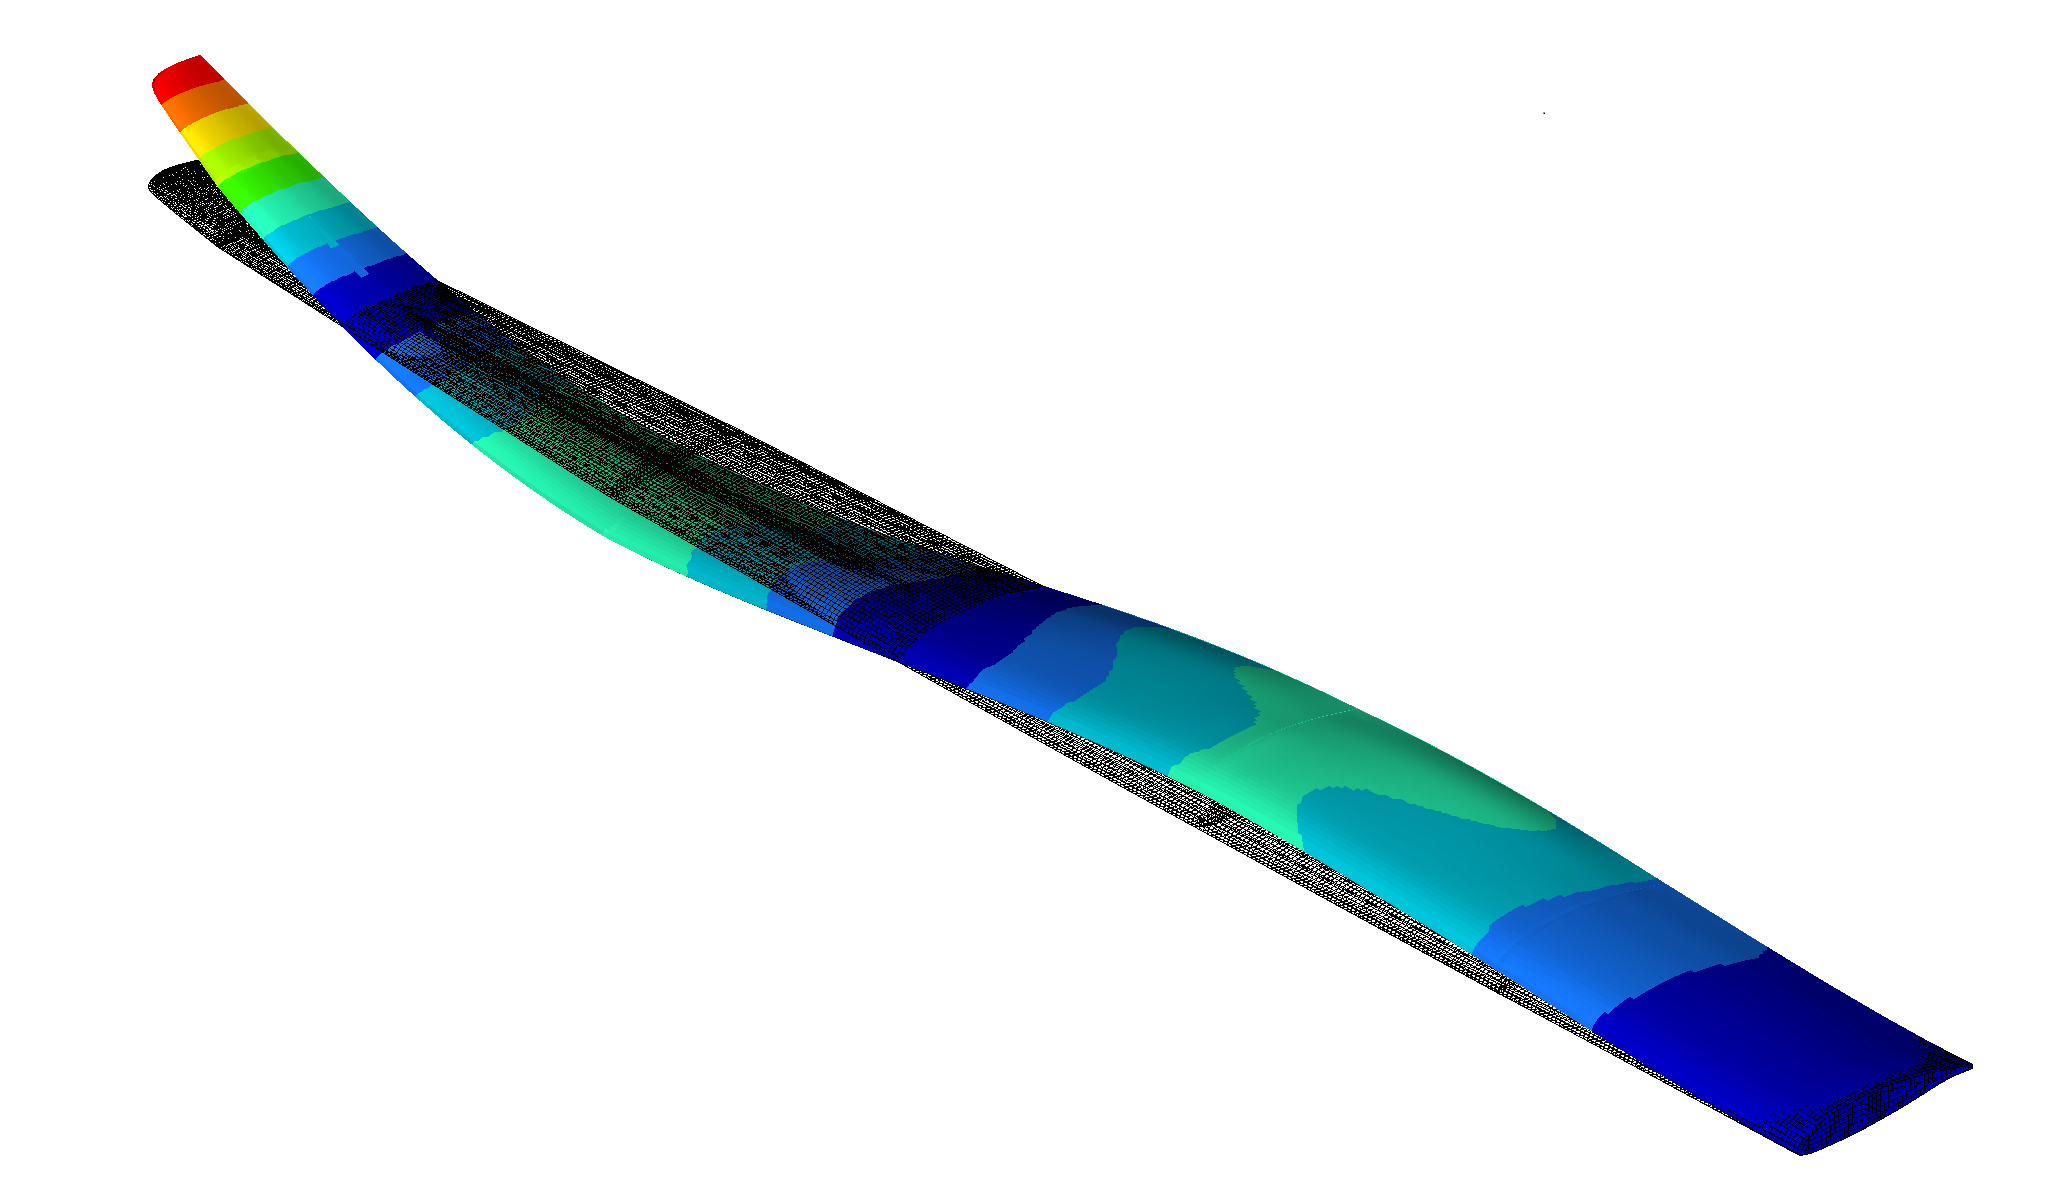
\includegraphics[width=0.8\paperwidth]{mode4_17.386Hz.png}}
  \end{picture}
  
  % \end{center}


    \begin{figure}[H]
      \begin{center}
        
\includegraphics[width=3cm]{LogoAUTH.png}
        \label{fig:cover_auth_logo}
      \end{center}
    \end{figure}
    
   \begin{center}
    
    \large Aristotle University of Thessaloniki\\
    \normalsize Department of Mechanical Engineering\\

    
    \vspace{0.7in}
    
    \LARGE\textbf{Aeroelastic Flutter Optimization of Wing Structures}
    
    \vspace{3in}
    
    \Large Xenodochidis Vasileios
    
    \end{center}
    
    \vfill

    \large

    \begin{tabular}{ccc}
        \textbf{Supervisors:} &Giagkopoulos Dimitrios, & Associate Proffesor.\\
        & Koutsoupakis Josef, & Ph.D. Candiadate

    \end{tabular}
    \vspace{1in}

    
    \centering
    \today
    
\end{titlepage}
\restoregeometry
    
    \begin{abstract}
    Η παρούσα διπλωματική εργασία παρουσιάζει μια αεροελαστική ανάλυση μιας
    πτέρυγας, με στόχο τη βελτιστοποίηση του πολυστρωματικoύ σύνθετου υλικού
    της για τη μεγιστοποίηση της ταχύτητας πτερυγισμού ελαχιστοποιώντας
    παράλληλα τη μάζα. Η μελέτη χρησιμοποιεί τον επιλυτή \textlatin{OptiStruct} της
    \textlatin{Altair} για να αξιολογήσει την αεροελαστική σταθερότητα της δομής.
    Διάφοροι αλγόριθμοι βελτιστοποίησης, που υλοποιήθηκαν στην \textlatin{Python},
    χρησιμοποιήθηκαν για να εξερευνήσουν το χώρο σχεδιασμού και να
    εντοπίσουν βέλτιστους συνδυασμούς παραμέτρων που παράγουν αποδεκτά
    χαρακτηριστικά πτερυγισμού ενώ ταυτόχρονα ελαχιστοποιούν τη μάζα της
    κατασκευής. Επιπλέον, αναπτύχθηκε ένα μοντέλο νευρωνικού δικτύου για την
    πρόβλεψη της ταχύτητας πτερυγισμού με βάση βασικές δομικές και υλικές
    παραμέτρους, για να αναδειχθούν οι δυνατότητες που έχει ένα υποκατάστατο
    μοντέλο στην πρόβλεψη της ταχύτητας πτερυγισμού. Τα αποτελέσματα
    δείχνουν σημαντικές βελτιώσεις τόσο στην ταχύτητα πτερυγισμού όσο και
    στη μείωση βάρους, τονίζοντας τις δυνατότητες των προηγμένων τεχνικών
    βελτιστοποίησης και της μηχανικής μάθησης στον αεροελαστικό σχεδιασμό.
\end{abstract}

\selectlanguage{english}
\begin{abstract}
    This thesis presents an aeroelastic analysis of a wing structure with
    the objective of optimizing its composite material to maximize flutter
    speed while minimizing mass. The study utilizes Altair's OptiStruct
    solver to compute flutter curves and assess the aeroelastic stability of
    the structure. Various optimization algorithms, implemented in Python,
    were employed to explore the design space and identify optimal
    configurations that balance structural mass and aeroelastic performance.
    Furthermore, a neural network model was developed to predict flutter
    speed based on key structural and material parameters, to see the
    potential that a surrogate model has in predicting the flutter speed.
    The results demonstrate significant improvements in both flutter speed
    and weight reduction, highlighting the potential of advanced
    optimization techniques and machine learning in aeroelastic design.
\end{abstract}


    \selectlanguage{english}

    \pagestyle{plain}
    \tableofcontents
    
    \listoffigures    
    \listoftables

    \pagestyle{fancy}
    \clearpage
    \setcounter{page}{1}
    \pagenumbering{arabic}

    \setcounter{chapter}{0}
\chapter{Introduction}\label{introduction}

\chapterprecis{
The Introduction chapter describes the aim of the thesis. It also
defines the limits and scope of this work. Finally, it describes the
motivation behind this project.}

\section{Problem Statement}\label{problem-statement}

Aeroelasticity is a branch of physics and engineering which studies the
response of elastic bodies exposed to a fluid flow. The forces involved
in this interaction are inertial, elastic and aerodynamic. Aeroelastic
problems in engineering can be classified into two broad categories:
static aeroelasticity which deals with the steady state response, and
dynamic aeroelasticity dealing mainly with the body's vibrational
response.

The most common aeroelastic effects encountered by aircraft are:

\begin{itemize}
\item
  \emph{Aerodynamic Divergence}, where the deflection of lifting
  surfaces of an aircraft leads to additional lift that, in turn, leads
  to further deflection in the same direction, resulting in excessive
  stress or even leading to structural failure
\item
  \emph{Aeroelastic Control reversal,} where the forces generated by the
  control aileron (responsible for the roll control of an aircraft) are
  sufficient to twist the wing itself to such an extent that it changes
  the lift characteristics of the wing which makes the control surfaces
  ineffective or even produces the opposite of the expected result
\item
  \emph{Aeroelastic Flutter} is a dynamic instability of a structure
  that occurs due to the interaction of the fluid flow with the
  eigenmodes of the structure
\end{itemize}

In this thesis the flutter characteristics of a lifting surface will be
explored and tailored to specific requirements using optimization
techniques.

\section{Objective}\label{objective}

The objective of this project is to develop an understanding of the
flutter characteristics of a lifting surface made of a laminate
composite material and the methods used to computationally predict the
flutter region using Altair's Optistruct solver. Thereafter the effect
of several structural parameters is studied to determine their effect on
the flutter characteristics and the effectiveness of several
optimization techniques is tested to tailor the flutter characteristics
to a set of requirements using Python.

\section{Scope and Limitations}\label{scope-and-limitations}

The project will include:

\begin{itemize}
\item
  The study of composite materials and their implementation in the
  Optistruct solver
\item
  The study of the Vortex Lattice panel Method and how it is used during
  the Aerodynamic Flutter Analysis
\item
  The study of Aeroelastic Flutter Analysis on a theoretical basis by
  means of the governing equations of motion and on a computational
  basis by studying the implementation of theory into commercial
  solvers.
\item
  Investigation of the effect of composite material properties on the
  flutter characteristics
\item
  Investigation of different optimization techniques to manipulate the
  flutter characteristics including line search methods, genetic
  algorithms and Neural Networks
\end{itemize}

\section{Motivation}\label{motivation}

In the aerospace industry minimization of weight of structures is of
utmost importance, since it allows the increase of useful payload,
improves efficiency maneuverability and other control characteristics. A
consequence of structural weight minimization is the reduction of safety
margins in comparison to other engineering fields, thus the need for
more precise calculations arises to ensure safety.

As aerospace prototype testing costs are elevated, computer simulations
are used more and more and become ever more advanced with the ability to
study a wider range of phenomena. This project would help students and
researchers understand the basics of wing flutter instability and
provide insight into the optimization process for such structures. The
code developed in this project could also be extended and modified by
anyone tackling a similar project.

    
\chapter{Theoretical Background}
\label{Ch:Theory}
\chapterprecis{In this next chapter the basic theory which will be used during this project is presented. There are four main sections in this chapter. The first three sections are involved in solving for a lifting surface's flutter characteristics while the fourth section presents the various optimization techniques that will be used.}

\section{Composite Finite Elements}\label{composite-finite-elements}

The theory behind the composite structural elements is developed according to E. Oñate, Structural Analysis with the Finite Element Method \cite{onate2013} which provides the basic equations and assumptions needed to develop 2D shell finite elements that take into account the effect of multilayer laminate composite materials.

\subsection{Displacement Field}\label{displacement-field}

When studying composite laminated plate elements, the main problem that arises is that in contrast to homogeneous materials, points that belong on the middle plane of the element can be displaced ``in plane'' this results in axial forces that are not possible within a homogeneous material. To account for this fact, we introduce two axial displacements $u_0(x,y)$ and $v_0(x,y)$ and thus the displacement of any point within the plate can be calculated as follows:
\begin{subequations}
    \label{eq:disp_field}
    \begin{equation}
        u(x,y,z)=u_0(x,y) -z\theta_x (x,y)
    \end{equation}
    \begin{equation}
        v(x,y,z)=v_0(x,y) -z\theta_y (x,y)
    \end{equation}
    \begin{equation}
        w(x,y,z)=w_0 (x,y)
    \end{equation}
\end{subequations}

\begin{figure}[h]
  \centering
  \includesvg[width=\textwidth]{plate element axes.svg}
  \caption{Composite element coordinate system}
\end{figure}



\subsection{Strain vectors}
\label{strain-vectors}

The strain within the plate can be calculated as follows:

\begin{align}
    \label{eq:strain}
  \boldsymbol{\epsilon} &= 
  \begin{bmatrix}[1.2]
  \frac{\partial u}{\partial x} \\
  \frac{\partial v}{\partial y} \\
  \frac{\partial u}{\partial y} + \frac{\partial v}{\partial x} \\
  \frac{\partial u}{\partial z} + \frac{\partial w}{\partial x} \\
  \frac{\partial v}{\partial z} + \frac{\partial w}{\partial y}
  \end{bmatrix}
  \notag \\&=
  \begin{bmatrix}[1.2]
  \frac{\partial u_{0}}{\partial x} \\
  \frac{\partial v_{0}}{\partial y} \\
  \frac{\partial u_{0}}{\partial y} + \frac{\partial v_{0}}{\partial x} \\
  0 \\
  0
  \end{bmatrix}
  +
  \begin{bmatrix}[1.2]
  - z\frac{\partial\theta_{x}}{\partial x} \\
  - z\frac{\partial\theta_{y}}{\partial y} \\
  - z\left( \frac{\partial\theta_{x}}{\partial y} + \frac{\partial\theta_{y}}{\partial x} \right) \\
  \frac{\partial w_{0}}{\partial x} - \theta_{x} \\
  \frac{\partial w_{0}}{\partial y} - \theta_{y}
  \end{bmatrix}
  \notag \\&= 
  \begin{bmatrix}[1.2]
  \hat{\boldsymbol{\epsilon}}_{m} \\
  \mathbf{0}
  \end{bmatrix}
  +
  \begin{bmatrix}[1.2]
  - z \cdot \hat{\boldsymbol{\epsilon}}_{b} \\
  \hat{\boldsymbol{\epsilon}}_{s}
  \end{bmatrix}
  =
  \mathbf{S} \cdot \hat{\boldsymbol{\epsilon}}
\end{align}
  

Where:
$$
    \boldsymbol{\epsilon} =
    \begin{bmatrix}[1.2]
    \widehat{\boldsymbol{\epsilon}}_{m} \\
    \widehat{\boldsymbol{\epsilon}}_{b} \\
    \widehat{\boldsymbol{\epsilon}}_{s}
    \end{bmatrix}, \quad
    \widehat{\boldsymbol{\epsilon}}_{m} =
    \begin{bmatrix}[1.2]
    \frac{\partial u_{0}}{\partial x} \\
    \frac{\partial v_{0}}{\partial y} \\
    \frac{\partial u_{0}}{\partial y} + \frac{\partial v_{0}}{\partial x}
    \end{bmatrix}, \quad
    \widehat{\boldsymbol{\epsilon}}_{b} =
    \begin{bmatrix}[1.2]
    \frac{\partial\theta_{x}}{\partial x} \\
    \frac{\partial\theta_{y}}{\partial y} \\
    \frac{\partial\theta_{x}}{\partial y} + \frac{\partial\theta_{y}}{\partial x}
    \end{bmatrix}, \quad
    \widehat{\boldsymbol{\epsilon}}_{s} =
    \begin{bmatrix}[1.2]
    \frac{\partial w_{0}}{\partial x} - \theta_{x} \\
    \frac{\partial w_{0}}{\partial y} - \theta_{y}
    \end{bmatrix}
$$

Are the generalized Stress vectors due to membrane (m), bending (b) and
transverse (s) shear deformation effects.
\begin{equation}
    S =
    \begin{bmatrix}
    I_{3} & - z I_{3} & O_{2} \\[5pt]
    O_{3}^{T} & O_{2} & I_{2}
    \end{bmatrix}
\end{equation}

Where, $ I_{n} $ is the $n \times n$ identity matrix, and

\[
O_{2} =
\begin{bmatrix}
0 & 0 \\
0 & 0
\end{bmatrix}, \quad
O_{3} =
\begin{bmatrix}
0 & 0 \\
0 & 0 \\
0 & 0
\end{bmatrix}.
\]


From the preceding relationship we can extract the following useful expressions:

\begin{equation}
    \boldsymbol{\epsilon} = 
    \begin{bmatrix}
        \boldsymbol{\epsilon}_{\mathbf{p}} \\
        \boldsymbol{\epsilon}_{\mathbf{s}}
    \end{bmatrix}
\end{equation}

Where: 
$\boldsymbol{\epsilon}_{\mathbf{p}} = 
\begin{bmatrix}
\epsilon_{x} \\
\epsilon_{y} \\
\epsilon_{z}
\end{bmatrix} = \ {\hat{\boldsymbol{\epsilon}}}_{\mathbf{m}}\mathbf{-}z{\hat{\boldsymbol{\epsilon}}}_{\mathbf{b}}$
,\quad
$\boldsymbol{\epsilon}_{\mathbf{s}}=\begin{bmatrix}
\gamma_{xy} \\
\gamma_{yz}
\end{bmatrix}={\hat{\boldsymbol{\epsilon}}}_{\mathbf{s}}
$

\subsection{Stress -- Strain
relationship}\label{stress-strain-relationship}


The stress strain relationship in a composite laminated plate will now be derived.

We consider a composite laminated plate formed by piling $n_{l}$
orthotropic layers called plies with orthotropy axes $L,T,z$ and isotropy
in the $L$ axis (the $Tz$ plane). The $L$ axis is parallel to the direction of
the longitudinal fibers of the composite material.

It will be assumed that:

\begin{itemize}
\item
  Each layer (k) is defined by the plane $z = z_{k}$ and
  $z = z_{k + 1}$ with $z_{k} \leq z \leq z_{k + 1}$
\item
  The Orthotropy axes L and T can vary for each layer and are
  represented by angle $\beta_{i}$ defined to be the angle between the
  global x axis and the $L_{i}$ axis of the ith layer
\item
  Each layer satisfies the plane stress assumption, namely
  $\sigma_{z} = 0$ and that the z axis is the orthotropy axis common
  for all layers
\item
  The displacement field is continuous between the layers and satisfies \eqref{eq:disp_field}
\end{itemize}

\begin{figure}[h]
    \centering
    \includegraphics[width=0.7\textwidth]{"composite layers definition.png"}
    \caption{Definition of layers in a composite laminated plate \cite{onate2013}}
    \label{fig:composite_layers}
\end{figure}


The assumptions stated above allow us to express the relationship
between the in-plane stresses $\sigma_{x},\ \sigma_{y},\ \tau_{xy}$
and the transverse shear strains $\tau_{xz},\tau_{yz}$ with their
corresponding strains for each layer k as follows:
\begin{equation}
    \boldsymbol{\sigma}_{\mathbf{p}} =
    \begin{bmatrix}
        \sigma_{x} \\
        \sigma_{y} \\
        \tau_{xy}
    \end{bmatrix} \\
    = \mathbf{D_p}
    \begin{bmatrix}
        \epsilon_{x} \\
        \epsilon_{y} \\
        \gamma_{xy}
    \end{bmatrix} \\
    = \mathbf{D_p} \boldsymbol{\epsilon}_{p}
\end{equation}
    

\begin{equation}
    \boldsymbol{\sigma}_{\mathbf{s}} = \begin{bmatrix}
    \tau_{xz} \\
    \tau_{yz}
    \end{bmatrix} \\
    = \mathbf{D}_{\mathbf{s}} \begin{bmatrix}
    \gamma_{xz} \\
    \gamma_{yz}
    \end{bmatrix} \\
    = \mathbf{D}_{\mathbf{s}} \boldsymbol{\epsilon}_{s}
    \end{equation}
    

And finally
\begin{equation}
\begin{array}{r}
\boldsymbol{\sigma}=\begin{bmatrix}
\boldsymbol{\sigma_p} \\
\boldsymbol{\sigma_s}
\end{bmatrix}=\begin{bmatrix}
\mathbf{D}_{\mathbf{p}} & \mathbf{0} \\
\mathbf{0} & \mathbf{D_s}
\end{bmatrix}\mathbf{\cdot}\begin{bmatrix}
\boldsymbol{\epsilon_{p}} \\
\boldsymbol{\epsilon}_{\mathbf{s}}
\end{bmatrix}=\boldsymbol{D\epsilon}
\end{array}
\end{equation}



The constitutive matrices $\mathbf{D_{p}, D_{s}}$ are symmetrical and their
terms are a function of the five independent material properties as well
as the angle $\beta_{k}$. The calculation of the aforementioned
matrices begins by expressing the stress -- strain relationships in the
orthotropy axes $L, T, z$

\begin{equation}    
\begin{array}{r}
\sigma_{1} = \mathbf{D}_{\mathbf{1}}\epsilon_{1},\ \ \sigma_{2} = \mathbf{D}_{\mathbf{2}}\epsilon_{2}
\end{array}
\end{equation}

Where:
\begin{center}

$\sigma_{1} = \begin{bmatrix}
\sigma_{L} \\
\sigma_{T} \\
\tau_{LT}
\end{bmatrix},\ \ \epsilon_{1} = \begin{bmatrix}
\epsilon_{L} \\
\epsilon_{T} \\
\gamma_{LT}
\end{bmatrix},\ \ \mathbf{D}_{\mathbf{1}}=\begin{bmatrix}
D_{LL} & D_{LT} & 0 \\
\  & D_{TT} & 0 \\
Sym. & \  & G_{LT}
\end{bmatrix}$

\vspace{10pt}
$\sigma_{2} = \begin{bmatrix}
\tau_{Lz} \\
\tau_{Tz}
\end{bmatrix},\ \ \epsilon_{2} = \begin{bmatrix}
\gamma_{Lz} \\
\gamma_{Tz}
\end{bmatrix},\ \ \mathbf{D}_{\mathbf{2}}=\begin{bmatrix}
G_{Lz} & 0 \\
0 & G_{Tz}
\end{bmatrix}$
\end{center}

\[D_{LL} = \frac{E_{L}}{a},\ \ D_{TT} = \frac{E_{T}}{a},\ \ a = 1 - \nu_{LT}\nu_{TL},\ \ D_{LT} = \frac{E_{T}\ \nu_{LT}}{a}\]

The most commonly used five independent material parameters are:

\[E_{L},\ \ E_{T},\ \ \nu_{LT}\left( or\ \nu_{TL} = \frac{E_{T}}{E_{L}}\nu_{LT} \right),\ \ G_{Lz} = G_{LT},\ \ G_{Tz}\]

Finally, the relationship between matrices $D_{1},{\ D}_{2}$ and
$D_{p},\ \ D_{s}$ can be expressed as a simple matrix product with
transformation matrices $T_{1}\ and\ T_{2}$ as follows:

\begin{equation}    
D_{p} = T_{1}^{T} \cdot D_{1} \cdot T_{1},\ \ D_{s} = T_{2}^{T} \cdot D_{2} \cdot T_{2}
\end{equation}

Where:

\[T_{1} = \begin{bmatrix}
\cos^{2}\left( \beta_{k} \right) & \sin^{2}\left( \beta_{k} \right) & \cos\left( \beta_{k} \right)sin(\beta_{k}) \\
\sin^{2}\left( \beta_{k} \right) & \cos^{2}\left( \beta_{k} \right) & - \cos\left( \beta_{k} \right)sin(\beta_{k}) \\
 - {2cos}{\left( \beta_{k} \right)\sin\left( \beta_{k} \right)} & {2cos}{\left( \beta_{k} \right)\sin\left( \beta_{k} \right)} & \cos^{2}\left( \beta_{k} \right) - \sin^{2}\left( \beta_{k} \right)
\end{bmatrix}\]

\[T_{2} = \begin{bmatrix}
\cos\left( \beta_{k} \right) & \sin\left( \beta_{k} \right) \\
 - \sin\left( \beta_{k} \right) & \cos\left( \beta_{k} \right)
\end{bmatrix}\]


\subsection{Generalized Constitutive Matrix}
\label{generalized-constitutive-matrix}
\begin{equation}
{\hat{\boldsymbol{\sigma}}}_{m} = \begin{bmatrix}
N_{x} \\
N_{y} \\
N_{xy}
\end{bmatrix} = \int_{- \frac{t}{2}}^{\frac{t}{2}}{\boldsymbol{\sigma}_{\mathbf{p}}dz},\ \ membrane\ forces
\end{equation}

\begin{equation}    
{\hat{\boldsymbol{\sigma}}}_{b} = \begin{bmatrix}
M_x \\
M_y \\
M_{xy}
\end{bmatrix} = - \int_{- \frac{t}{2}}^{\frac{t}{2}}{z\boldsymbol{\sigma}_{\mathbf{p}}dz},\ \ Bending\ moments
\end{equation}

\begin{equation}
    \hat{\boldsymbol{\sigma}}_{s} = \begin{bmatrix}
    Q_x \\
    Q_y
    \end{bmatrix} = \int_{-\frac{t}{2}}^{\frac{t}{2}} z \boldsymbol{\sigma}_{\mathbf{s}} \, dz \quad \text{transverse shear forces}
\end{equation}
    
\begin{align}
    \hat{\boldsymbol{\sigma}}_{m} &= {\hat{\mathbf{D}}}_{m}{\hat{\epsilon}}_{m} + {\hat{\mathbf{D}}}_{mb}{\hat{\epsilon}}_{b} \\
    \hat{\boldsymbol{\sigma}}_{b} &= {\hat{\mathbf{D}}}_{mb}{\hat{\epsilon}}_{m} + {\hat{\mathbf{D}}}_{b}{\hat{\epsilon}}_{b} \\
    \hat{\boldsymbol{\sigma}}_{s} &= {\hat{\mathbf{D}}}_{s}{\hat{\epsilon}}_{s}
\end{align}
    

Where:
\begin{equation}
    \label{eq:Dm}
\begin{array}{r}
{\hat{\mathbf{D}}}_{m} = \int_{- t/2}^{t/2}{\mathbf{D}_{p}dz} 
\end{array}
\end{equation}


\begin{equation} 
    \label{eq:Dmb}  
\begin{array}{r}
{\hat{\mathbf{D}}}_{mb} = \int_{- t/2}^{t/2}{z\mathbf{D}_{p}dz}
\end{array}
\end{equation}

\begin{equation}
    \label{eq:Db}
\begin{array}{r}
{\hat{\mathbf{D}}}_{b} = \int_{- t/2}^{t/2}{z^{2}\mathbf{D}_{p}dz}\
\end{array}
\end{equation}


\begin{equation}
    \label{eq:Dshear}    
\hat{\mathbf{D}}_{\mathbf{s}} =
\begin{bmatrix}
k_{11} \overline{D}_{s_{11}} & k_{12} \overline{D}_{s_{12}} \\
\text{Sym} & k_{22} \overline{D}_{s_{22}}
\end{bmatrix}, \quad
\text{with} \quad
\overline{D}_{s_{ij}} = \int_{- \frac{t}{2}}^{\frac{t}{2}} D_{s_{ij}} \, dz
\end{equation}




In equation \eqref{eq:Dshear} the $k_{ij}$ terms are called the shear
correction factors

The integrals in the equations \eqref{eq:Dm} - \eqref{eq:Dshear} can be expressed as a finite sum
when the composite laminate plate consists of $n_{l}$ orthotropic
layers. For composite plates where x and y are orthotropy axes for all
the layers the ${\hat{\mathbf{D}}}_{\mathbf{s}}$ ,matrix is
diagonal and only $k_{11}$ and $k_{22}$ need to be computed.
\\
The simplest method of computing the shear stress factors is by assuming
cylindrical bending. This means that:
\begin{equation}
\frac{\partial\sigma_{x}}{\partial x} + \frac{\partial\tau_{xz}}{\partial z} = 0\ 
\end{equation}

Further assuming a constant distribution of the transverse shear stress
in the thickness direction and after some manipulation it is finally
deduced

\begin{equation}
k_{11} = {\hat{D}}_{b_{11}}^{2}\left\lbrack {\overline{G}}_{xz}\int_{- t\text{/}2}^{t\text{/}2}{\frac{g_{1}^{2}(z)}{G_{xz}}dz} \right\rbrack^{- 1}
\end{equation}

\begin{equation}
k_{22} = {\hat{D}}_{b_{22}}^{2}\left\lbrack {\overline{G}}_{yz}\int_{- t\text{/}2}^{t\text{/}2}{\frac{g_{2}^{2}(z)}{G_{yz}}dz} \right\rbrack^{- 1}
\end{equation}

Where:

\begin{align*}
  g_{1(z)} &= \int_{- t\text{/}2}^{z}{zD_{p_{11}}dz}\\
  g_{2(z)} &= \int_{- t\text{/}2}^{z}{zD_{p_{22}}dz}\\
  {\overline{G}}_{xz} &= \int_{- t\text{/}2}^{t\text{/}2}G_{xz}dz\\
  {\overline{G}}_{yz} &= \int_{- t\text{/}2}^{t\text{/}2}G_{yz}dz
\end{align*}


Equations \eqref{eq:Dm} through \eqref{eq:Dshear} can be expressed as a finite sum when
the laminate composite is made of $n_{l}$ orthotropic layers within
each of which the material properties are constant

\begin{equation}
{\hat{\mathbf{D}}}_{m} = \sum_{k = 1}^{n_{l}}{t_{k}\mathbf{D}_{pk}}
\end{equation}

\begin{equation}
{\hat{\mathbf{D}}}_{mb} = - \sum_{k = 1}^{n_{l}}{t_{k}{\overline{z_{k}}\mathbf{D}}_{pk}}
\end{equation}

\begin{equation}
    \hat{\mathbf{D}}_{b} = \sum_{k = 1}^{n_{l}} \frac{1}{3} \left( \overline{z}_{k + 1}^{3} - z_{k}^{3} \right) \mathbf{D}_{pk}
\end{equation}


\begin{equation}
\ {\hat{\mathbf{D}}}_{\mathbf{s}}=\begin{bmatrix}
{\widetilde{k}}_{11}\ \sum_{k = 1}^{n_{l}}{t_{k}\mathbf{D}_{sk_{11}}}\ \ \  & 0 \\
0 & {\widetilde{k}}_{22}\sum_{k = 1}^{n_{l}}{t_{k}\mathbf{D}_{sk_{22}}}
\end{bmatrix}
\end{equation}

Where:

\[t_{k} = z_{k + 1} - z_{k},\ \ {\overline{z}}_{k} = \frac{1}{2}\left( z_{k + 1} + z_{k} \right)\]

\[{\widetilde{k}}_{ii} = {\hat{\mathbf{D}}}_{b_{ii}} \cdot \left\lbrack \sum_{k = 1}^{n_{l}}{t_{k}G_{xz}} \cdot \sum_{k = 1}^{n_{l}}\left( \frac{\sum_{l = 1}^{k}\left( t_{k}{\overline{z}}_{k}\mathbf{D}_{p_{{ii}_{l}}} \right)}{G_{xz_{k}}}t_{k} \right) \right\rbrack,\ \ i = 1,\ 2\]

\subsection{\texorpdfstring{Discretized stress and strain - Shape functions}{Discretized stress and strain - Shape functions}}\label{discretized-stress-and-strain---shape-functions}


The displacements within a four-node quadrilateral composite element can
be expressed through shape functions.

\begin{equation}
\mathbf{u} = \begin{bmatrix}
u \\
v \\
w \\
\theta_{x} \\
\theta_{y}
\end{bmatrix} = \sum_{i = 1}^{4}{N_{i}a_{i}} = \mathbf{N \cdot}\vec{\mathbf{a}}
\end{equation}

Where:

\[
\mathbf{N} = \begin{bmatrix} \mathbf{N_1} \mid \mathbf{N_2} \mid \mathbf{N_3} \mid \mathbf{N_4} \end{bmatrix}
\]

\[
\mathbf{N_i} =  
  \begin{bmatrix}
      N_i & 0 & 0 & 0 & 0  \\
      0 & N_i & 0 & 0 & 0  \\
      0 & 0 & N_i & 0 & 0  \\
      0 & 0 & 0 & N_i & 0  \\
      0 & 0 & 0 & 0 & N_i 
  \end{bmatrix}, \quad for \ i \in \{1,2,3,4\}
\]



\[\vec{\mathbf{a}}=\begin{bmatrix}
{\vec{\mathbf{a}}}_{\mathbf{1}} \\
{\vec{\mathbf{a}}}_{\mathbf{2}} \\
{\vec{\mathbf{a}}}_{\mathbf{3}} \\
{\vec{\mathbf{a}}}_{\mathbf{4}}
\end{bmatrix}=\begin{bmatrix}
u_{1} \\
v_{1} \\
w_{1} \\
\theta_{x_{1}} \\
\theta_{y_{1}} \\
u_{2} \\
v_{2} \\
w_{2} \\
\theta_{x_{2}} \\
\theta_{y_{2}} \\
u_{3} \\
v_{3} \\
w_{3} \\
\theta_{x_{3}} \\
\theta_{y_{3}} \\
u_{4} \\
v_{4} \\
w_{4} \\
\theta_{x_{4}} \\
\theta_{y_{4}}
\end{bmatrix}\]

The stress strain relationship using equation \eqref{eq:strain} can now be
expressed using the shape functions:

\begin{multline}
\boldsymbol{\epsilon} = \begin{bmatrix}
{\hat{\boldsymbol{\epsilon}}}_{m} \\
{\hat{\boldsymbol{\epsilon}}}_{b} \\
{\hat{\boldsymbol{\epsilon}}}_{s}
\end{bmatrix} = \begin{bmatrix}[1.3]
\frac{\partial u_{0}}{\partial x} \\
\frac{\partial v_{0}}{\partial y} \\
\frac{\partial u_{0}}{\partial y} + \frac{\partial v_{0}}{\partial x} \\
\frac{\partial\theta_{x}}{\partial x} \\
\frac{\partial\theta_{y}}{\partial y} \\
\frac{\partial\theta_{x}}{\partial y} + \frac{\partial\theta_{y}}{\partial x} \\
\frac{\partial w_{0}}{\partial x} - \theta_{x} \\
\frac{\partial w_{0}}{\partial y} - \theta_{y}
\end{bmatrix} = \sum_{i = 4}^{4}\begin{bmatrix}[1.3]
\frac{\partial N_{i}}{\partial x}u_{i} \\
\frac{\partial N_{i}}{\partial x}v_{i} \\
\frac{\partial N_{i}}{\partial y}u_{i} + \frac{\partial N_{i}}{\partial x}v_{i} \\
\frac{\partial N_{i}}{\partial x}\theta_{x_{i}} \\
\frac{\partial N_{i}}{\partial y}\theta_{y_{i}} \\
\frac{\partial N_{i}}{\partial y}\theta_{x_{i}} + \frac{\partial N_{i}}{\partial x}\theta_{y_{i}} \\
\frac{\partial N_{i}}{\partial x}w_{i} - N_{i}\theta_{x_{i}} \\
\frac{\partial N_{i}}{\partial y}w_{i} - N_{i}\theta_{y_{i}}
\end{bmatrix}\\
= \left\lbrack \mathbf{B_1}\mid\mathbf{B_2}\mid\mathbf{B_3}\mid \mathbf{B_4}\right\rbrack \cdot \vec{\mathbf{a}} = \mathbf{B} \cdot \vec{\mathbf{a}}
\end{multline}


Where:

\[\mathbf{B}_{\mathbf{i}}=\begin{bmatrix}
\mathbf{B}_{\mathbf{m}_{\mathbf{i}}} \\
\mathbf{B}_{\mathbf{b}_{\mathbf{i}}} \\
\mathbf{B}_{\mathbf{s}_{\mathbf{i}}}
\end{bmatrix}\]


\[
\mathbf{B_{m_{i}}} =\begin{bmatrix}[1.3]

\frac{\partial N_{i}}{\partial x} & 0 & 0 & 0 & 0 \\
0 & \frac{\partial N_{i}}{\partial y} & 0 & 0 & 0 \\
\frac{\partial N_{i}}{\partial y} & \frac{\partial N_{i}}{\partial x} & 0 & 0 & 0
\end{bmatrix},\ \ 
\mathbf{B_{b_{i}}}=\begin{bmatrix}[1.3]
0 & 0 & 0 & - \frac{\partial N_{i}}{\partial x} & 0 \\
0 & 0 & 0 & 0 & - \frac{\partial N_{i}}{\partial y} \\
0 & 0 & 0 & - \frac{\partial N_{i}}{\partial y} & - \frac{\partial N_{i}}{\partial x}
\end{bmatrix},\]
\[
\mathbf{B_{s_{i}}}=\begin{bmatrix}[1.3]
0 & 0 & \frac{\partial N_{i}}{\partial x} & - N_{i} & 0 \\
0 & 0 & \frac{\partial N_{i}}{\partial y} & 0 & - N_{i}
\end{bmatrix}
\]


The shape functions used can vary but the simplest is the bilinear
quadrilateral element which uses linear shape functions for
interpolation. All calculations described in the preceding chapter are
carried out in a transformed coordinate space where every element is a
perfect square of side length two length units. This transformed space
is called the ``natural'' space. The shape functions are:
\begin{align}
  N_{i}(\xi,\eta) &= \frac{1}{4}(1 + a_{i} \cdot \xi)(1 + b_{i} \cdot \eta) \label{eq:N_i} \\
  \frac{\partial N_{i}(\xi,\eta)}{\partial\xi} &= \frac{1}{4}a_{i}\left( 1 + b_{i}\eta \right) \label{eq:dNdxi} \\
  \frac{\partial N_{i}(\xi,\eta)}{\partial\eta} &= \frac{1}{4}b_{i}\left( 1 + a_{i}\xi \right) \label{eq:dNdeta}
\end{align}
  
\begin{table}[h]
  \centering
  \renewcommand{\arraystretch}{1.5} % Adjust row height for better spacing
  \begin{tabular}{>{\columncolor[gray]{0.8}}c|c  c c c}
      \rowcolor[gray]{0.8}
      \hline
      $\mathbf{i}$ & $\mathbf{1}$ & $\mathbf{2}$ & $\mathbf{3}$ & $\mathbf{4}$ \\ 
      \hline
      $a_i$ & -1 & 1 & 1 & -1 \\ 
      $b_i$ & -1 & -1 & 1 & 1 \\ 
      \hline
  \end{tabular}
  \caption{Shape function coefficients} % Caption for the table
  \label{tab:coefficients} % Label for referencing in the document
\end{table}

The Jacobian of this transformation from physical to natural space is
defined as:

\begin{equation}
\mathcal{J} = 
\begin{bmatrix}[1.3]
\frac{\partial x}{\partial\xi} & \frac{\partial y}{\partial\xi} \\
\frac{\partial x}{\partial\eta} & \frac{\partial y}{\partial\eta}
\end{bmatrix}
\end{equation}


The derivatives of the shape functions in the physical space can then be
calculated as:
\begin{equation}
\begin{aligned}
\begin{bmatrix}[1.3]
\frac{\partial N_{i}}{\partial x} \\
\frac{\partial N_{i}}{\partial y}
\end{bmatrix} = \mathcal{J}^{- 1} \cdot \begin{bmatrix}[1.3]
\frac{\partial N_{i}}{\partial\xi} \\
\frac{\partial N_{i}}{\partial\eta}
\end{bmatrix}
\end{aligned}
\end{equation}

Finally, another property of the Jacobian is that its determinant
represents the scale of the transformation.
\begin{figure}
\centering
  
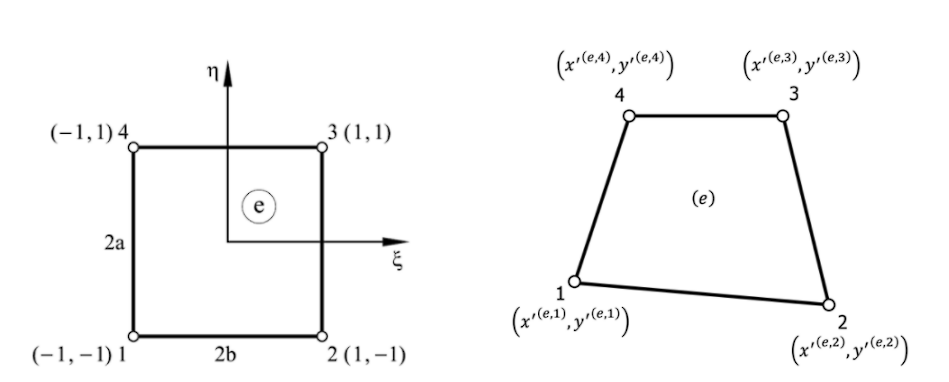
\includegraphics[scale=0.8]{nodes and coordinates of qudrilateral elements.png}
\caption{natural and physical coordinate space of quadrilateral plate element \cite{bolla2022}}
\end{figure}


\subsection{Stiffness matrix }\label{stiffness-matrix}

The final step in the computation of the finite elements is the
calculation and assembly of the stiffness matrix. Using the Principle of
Virtual Work in the standard manner the local stiffness matrices can be
written:

\begin{align}
  \mathbf{K}_{m_{ij}, [20 \times 20]} &= \iint_{Area} \mathbf{B}_{m,i}^{T}{\hat{\mathbf{D}}}_{m} \mathbf{B}_{m,j} \, dA, \quad \text{membrane stiffness} \label{Km} \\
  \mathbf{K}_{b_{ij}, [20 \times 20]} &= \iint_{Area} \mathbf{B}_{b,i}^{T}{\hat{\mathbf{D}}}_{b} \mathbf{B}_{b,j} \, dA, \quad \text{bending stiffness} \label{Kb}\\
  \mathbf{K}_{s_{ij}, [20 \times 20]} &= \iint_{Area} \mathbf{B}_{s,i}^{T}{\hat{\mathbf{D}}}_{s} \mathbf{B}_{s,j} \, dA, \quad \text{shear stiffness} \label{Ks}\\
  \mathbf{K}_{mb_{ij}, [20 \times 20]} &= \iint_{Area} \left( \mathbf{B}_{m,i}^{T}{\hat{\mathbf{D}}}_{mb} \mathbf{B}_{b,j} + \mathbf{B}_{b,i}^{T}{\hat{\mathbf{D}}}_{mb} \mathbf{B}_{m,j} \right) \, dA, \notag \\
  &\quad \hspace{4cm} \text{membrane-bending stiffness} \label{Kmb}
\end{align}

All the integrals in equations \eqref{Km} through \eqref{Kmb} are computed
using the Gauss quadrature. The full Gauss quadrature for the 4-node
plate element developed involves four integration points while the
reduced integration form of these elements requires only one Gauss
point.

\begin{figure}
    \centering
    \includesvg[width  = \textwidth]{full and reduced integration gauss points.svg}
    \caption{Gauss points for full and reduced Integration in 4 node elements}
\end{figure}


The Gaussian integration for two dimensional domains using $n$ Gauss
points states that:

\begin{equation}  
\int_{- 1}^{1}{\int_{- 1}^{1}{f(x,y)dxdy}} \approx \sum_{j = 1}^{n}{\sum_{i = 1}^{n}{w_{i}w_{j}f\left( x_{i},y_{i} \right),\ for\ every\ i,j \leq n}}
\end{equation}

Since the plate element has four nodes only two integrations are
possible:

\begin{itemize}
\item
  Using one Gauss point resulting in the reduced Integration scheme
\item
  Using four Gauss points resulting in the full integration scheme.
\end{itemize}


Using full integration results in greater computational time but
improves accuracy, on the other hand reduced integration make
computation faster requiring only a fourth as many computations, but
results in less accurate results and introduces the so called zero
energy modes which are deformed states of the element which have zero
strain energy. This is physically impossible and reduces the stiffness
of the structure as to achieve these modes of deformation no energy is
needed. This phenomenon is also known as the hourglass effect in FEM.

Table \ref{tab:GaussPoints}, exposes the Gauss point coordinates and the
weights that shall be used when performing one or four Gauss point
integration
\setlength{\tabcolsep}{20pt} % Increase column spacing (default is ~6pt)
\renewcommand{\arraystretch}{1.3}
\begin{table}[h]
    \centering
    \begin{tabular}{c | c c c c c}
        $N_G$ & $k$ & $w_k$ & $\xi_k$ & $\eta_k$ \\ \hline
        1 & 1 & 2 & 0 & 0 \\ \hline
        \multirow{4}{*}{4} & 1 & 1 & $-\frac{1}{\sqrt{3}}$ & $-\frac{1}{\sqrt{3}}$ \\
          & 2 & 1 & $+\frac{1}{\sqrt{3}}$ & $-\frac{1}{\sqrt{3}}$ \\
          & 3 & 1 & $+\frac{1}{\sqrt{3}}$ & $+\frac{1}{\sqrt{3}}$ \\
          & 4 & 1 & $-\frac{1}{\sqrt{3}}$ & $+\frac{1}{\sqrt{3}}$ \\
    \end{tabular}
    \caption{Gauss points weights and coordinates for one and four gauss point integration}
    \label{tab:GaussPoints}
\end{table}

Using the Gauss quadrature the local stiffness matrix of the plate
element can be calculated as the sum of all the component stiffness
matrices:

\begin{equation}
\mathbf{K}_{local} = \mathbf{K}_{m} + \mathbf{K}_{b} + \mathbf{K}_{s} + \mathbf{K}_{mb}
\end{equation}

The final step to obtain the global stiffness matrix is to transform the
local coordinate system back to the global coordinate system. This is
done using the rotation matrix and the determinant of the Jacobian as
the scale as follows:

\begin{equation}
\mathbf{K}_{global} = \det\left( \mathcal{J} \right) \cdot \mathbf{R}^{\mathbf{T}}\mathbf{\cdot}\mathbf{K}_{local} \cdot \mathbf{R}
\end{equation}

Where:

\[
\underset{\text{$5n \times 6n$}}{\mathbf{R}} =
\begin{bmatrix}
\mathbf{L}_{1} & \mathbf{0} & \mathbf{0} \\
\mathbf{0} & \ddots & \mathbf{0} \\
\mathbf{0} & \mathbf{0} & \mathbf{L}_{n}
\end{bmatrix}
\]



\[\mathbf{L_i}=
\begin{bmatrix}
\lambda_{x^{'}x}\ \  & \lambda_{x^{'}y} & \lambda_{x^{'}z} & 0 & 0 & 0 \\
\lambda_{y^{'}x} & \lambda_{y^{'}y} & \lambda_{y^{'}z} & 0 & 0 & 0 \\
\lambda_{z^{'}x} & \lambda_{z^{'}y} & \lambda_{z^{'}z} & 0 & 0 & 0 \\
0 & 0 & 0 & - \lambda_{y^{'}x} & - \lambda_{y^{'}y} & - \lambda_{y^{'}z} \\
0 & 0 & 0 & \lambda_{x^{'}x} & \lambda_{x^{'}y} & \lambda_{x^{'}z}
\end{bmatrix}\]


With $n = 4$ and $\lambda_{x^{'}x}\ $being the cosine of the angle
formed by axes $x'$ and $x$ etc.

\begin{figure}[H]
    \centering
    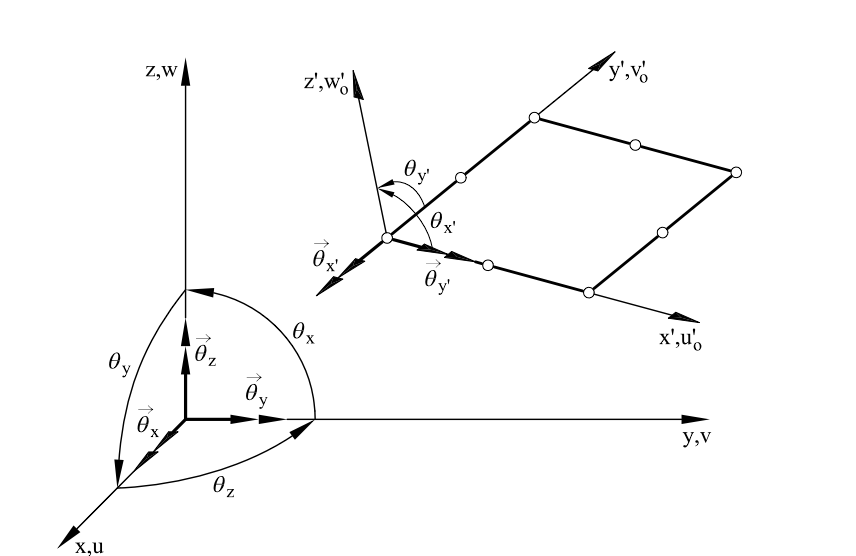
\includegraphics[width=\textwidth]{local and global axes of element .png}
    \caption{local and global axes definition \cite{onate2013}}
\end{figure}


The plate elements developed here only have 5 degrees of freedom per
node. In order to obtain the full six degrees of freedom per node a
stiffness component in the rotation about the z axis $\vartheta_{z}$
needs to be added. This is a fictitious stiffness term that can be added
to bring the stiffness matrix to its full size of $24 \times 24$. This
technique is often used to avoid potential singularities in the
stiffness matrix, and it is more intuitive for every node to have six
degrees of freedom.

A common technique used to avoid shear locking phenomenon is to
integrate the component stiffness matrices using different Gauss
quadrature.


\section[Aerodynamic Theory (VLM)]{Aerodynamic Theory -- Vortex Lattice Method (VLM)}
\label{aerodynamic-theory-vortex-lattice-method-vlm}

The vortex lattice method theory developed in this chapter follows the
conventions of the book A. P. Joseph Katz, Low-Speed Aerodynamics \cite{katz2001}




\subsection{The Vortex Filament -- Biot SavartLaw}
\label{the-vortex-filament-biot-savart-law}

\begin{figure}[H]
    \centering
    \includegraphics[width=0.8\textwidth]{vortex filament.png}
    \caption{Curved Three-dimensional vortex filament of strength $\Gamma$ \cite{pinzon2015}}
\end{figure}
% Curved Three-dimensional vortex filament of strength Γ

The continuity equation for an incompressible fluid is:

\begin{equation}
\nabla \cdot \vec{V} = 0
\end{equation}

The vector potential of the velocity field is a vector field

$\vec{B}$ which is defined by:

\begin{equation}
\nabla \times \vec{B} = \vec{V}
\end{equation}

The divergence of the vector potential $\vec{B}$ is zero
and thus the vorticity can be expressed as:

\begin{equation}
\boldsymbol{\zeta} = \nabla \times \vec{V} = \nabla \times \left( \nabla \times \vec{B} \right) = \cancel{\nabla\left( \nabla \cdot \vec{B} \right)} - \nabla^{2}\vec{B} = - \nabla^{2}\vec{B}
\end{equation}

\begin{figure}[H]
    \centering
    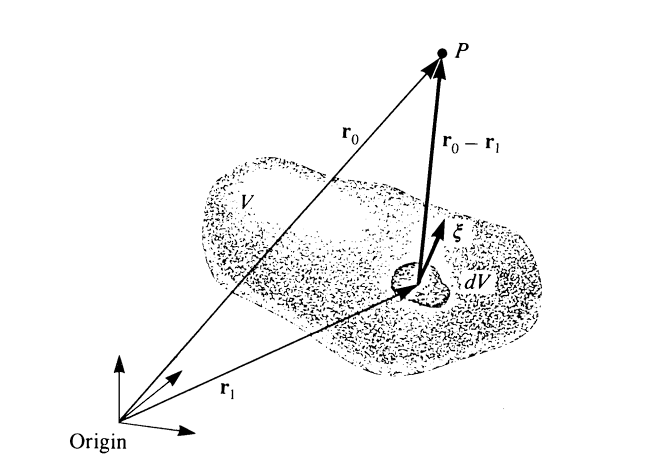
\includegraphics[width=0.8\textwidth]{induced velocity random vortex distribution.png}
    \caption{Velocity at point P due to a vortex distribution \cite{katz2001}}
\end{figure}

The general solution to this equation using greens theorem is:

\begin{equation}
    \label{eq:vortexvelocity}
\vec{B} = \frac{1}{4\pi}\int_{V}^{}{\frac{\vec{\zeta}}{\left| \vec{r} \right|}dV\ }
\end{equation}

\begin{equation}
\vec{V} = \frac{1}{4\pi}\int_{V}^{}{\nabla \times \frac{\vec{\zeta}}{\left| \vec{r} \right|}dV}
\end{equation}

Where:
\[\vec{r} = {\vec{r}}_{0} - {\vec{r}}_{1}\]


Considering an infinitesimal piece of vorticity filament $\zeta$ so
that:
\begin{equation}
d\mathbf{l} = \frac{\boldsymbol{\zeta}}{\zeta}dl, \quad \Gamma = \zeta \cdot dS,\quad dV = dS \cdot dl
\end{equation}

\begin{equation}
    \label{eq:ininitesimalvortex}
\nabla \times \frac{\zeta}{\left| \vec{r} \right|}d\vec{V} = \nabla \times \Gamma\frac{d\mathbf{l}}{\left| \vec{r} \right|} = \Gamma\frac{d\mathbf{l} \times \vec{r}}{\left| \vec{r} \right|^{3}}
\end{equation}


Substitution of equation \eqref{eq:vortexvelocity} into equation \eqref{eq:ininitesimalvortex} leads to

\begin{equation}
\vec{V} = \frac{1}{4\pi}\int_{V}^{}{\frac{d\mathbf{l} \times \vec{r}}{\left| \vec{r} \right|^{3}}dV\ }
\end{equation}



\subsection{Straight Vortex Segment}\label{straight-vortex-segment}

The vortex segment is placed at an arbitrary orientation with constant
circulation and finite length, as shown in \autoref{fig:InducedVelocityfromstraightVortexSegment}. As is
shown, the induced velocity has only a tangential component
$q_{\theta}$.

\begin{figure}[H]
    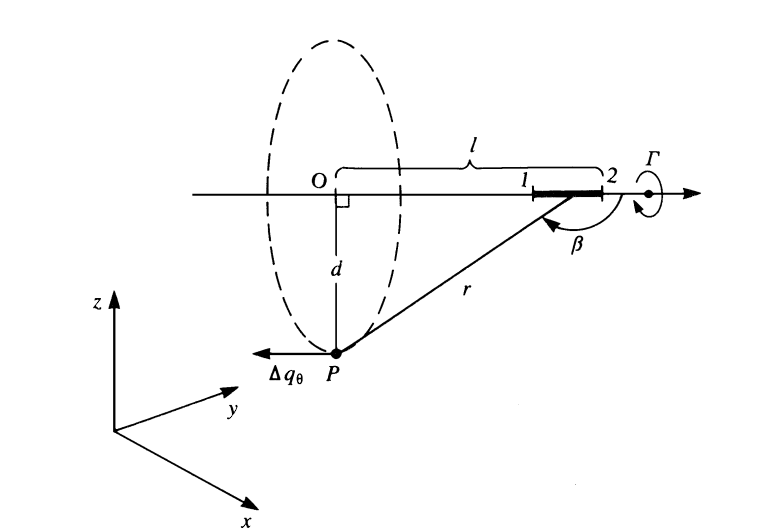
\includegraphics[width=0.8\textwidth]{finite vortex filament.png}
    \caption{Induced Velocity from straight Vortex Segment \cite{katz2001}}
    \label{fig:InducedVelocityfromstraightVortexSegment}
\end{figure}

From the analysis of the infinitesimal vortex filament, it has been
shown that the induced velocity is:

\begin{equation}
    \label{eq:inducedvelocity}
\Delta\mathbf{V =}\frac{\Gamma}{4\pi}\frac{d\mathbf{l} \times \vec{r}}{r^{3}} = \frac{\Gamma}{4\pi}\frac{\sin(\beta)}{r^{2}}dl\ \hat{e_{\theta}}
\end{equation}

Note that:

\[d = rsin(\beta)\quad \text{and} \quad \tan(\pi - \beta) = \frac{d}{l}\]

Therefore:

\[l = - \frac{d}{\tan(\beta)}\quad \text{and} \quad dl = \frac{d}{\sin^{2}(\beta)}d\beta\]

Substituting these terms in equation \eqref{eq:inducedvelocity} we get:

\begin{equation}
    \Delta V_{\theta} = \frac{\Gamma}{4\pi d}\sin(\beta)d\beta\
\end{equation}
This equation can be integrated over the straight vortex segment
resulting in:

\begin{equation}
{V_{\theta}}_{1 \rightarrow 2\ } = \frac{\Gamma}{4\pi d}\int_{\beta_{1}}^{\beta_{2}}{\sin(\beta)d\beta =}\frac{\Gamma}{4\pi d}\left( \cos\left( \beta_{1} \right) - cos\left( \beta_{2} \right) \right)
\end{equation}

\begin{figure}[H]
  \centering
  \begin{minipage}{0.49\textwidth}
      \centering
      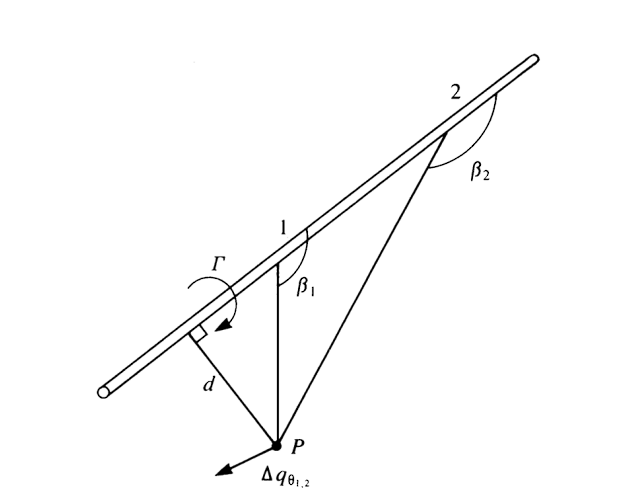
\includegraphics[width=\linewidth]{viewing angles straight vortex segment.png}
  \end{minipage}
  \hfill
  \begin{minipage}{0.49\textwidth}
      \centering
      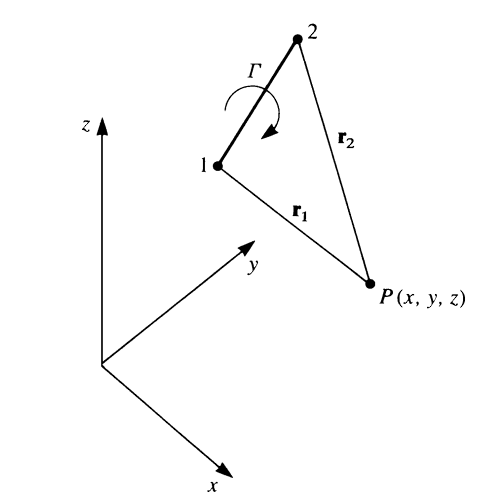
\includegraphics[width=\linewidth]{vortex segment vectors.png}

  \end{minipage}
  \caption{Vortex segment geometry \cite{katz2001}}
\end{figure}

Finally noting that:

\begin{align*}
  d &= \frac{\left| \vec{r}_1 \times \vec{r}_2 \right|}{|\vec{r}_0|}, \quad
  \cos\beta_1 = \frac{\vec{r}_0 \cdot \vec{r}_1}{|\vec{r}_0| |\vec{r}_1|} \\
  \cos\beta_2 &= \frac{\vec{r}_0 \cdot \vec{r}_2}{|\vec{r}_0| |\vec{r}_2|}, \quad
  \hat{e}_\theta = \frac{\vec{r}_1 \times \vec{r}_2}{\left| \vec{r}_1 \times \vec{r}_2 \right|}
\end{align*}



The induced velocity becomes:

\begin{equation}
    \label{eq:V12}
{\vec{V}}_{1 \rightarrow 2} = \frac{\Gamma}{4\pi}\ \frac{{\vec{r}}_{1} \times {\vec{r}}_{2}}{\left| {\vec{r}}_{1} \times {\vec{r}}_{2} \right|}\ ({\vec{r}}_{1} - {\vec{r}}_{2}) \cdot \left( \frac{{\vec{r}}_{1}}{\left| {\vec{r}}_{1} \right|} - \frac{{\vec{r}}_{2}}{\left| {\vec{r}}_{2} \right|} \right)
\end{equation}


\subsection{Lifting Surface Computational Solution by Vortex Ring
Elements}\label{lifting-surface-computational-solution-by-vortex-ring-elements}

The goal of this section is the calculation of the influence coefficient
matrix which is necessary to predict the lift of an oscillating wing
surface.

The main boundary condition that must be satisfied is the zero normal
flow across the wing's solid surface which can be expressed using the
velocity potential $\nabla\Phi = \vec{V}$ as:

\begin{equation}
\nabla\left( \Phi + \Phi_{\infty} \right) \cdot \hat{n} = 0
\end{equation}

The numerical method begins by defining the type of singularity element
that will be used. In the Vortex Lattice method, a Vortex ring is used.
The vortex ring is a quadrilateral element which has a straight vortex
line at every edge. The leading vortex is placed at the quarter chord of
the panel while the collocation point is at the center of the
three-quarter chord line. The normal vector of the panel is calculated
on the collocation point. A positive circulation $\Gamma$ is defined
according to the right-hand rule. By placing the leading-edge vortex at
the quarter-chord line the 2-dimension Kutta condition is satisfied
along the chord.

\begin{figure}[H]
  \centering
  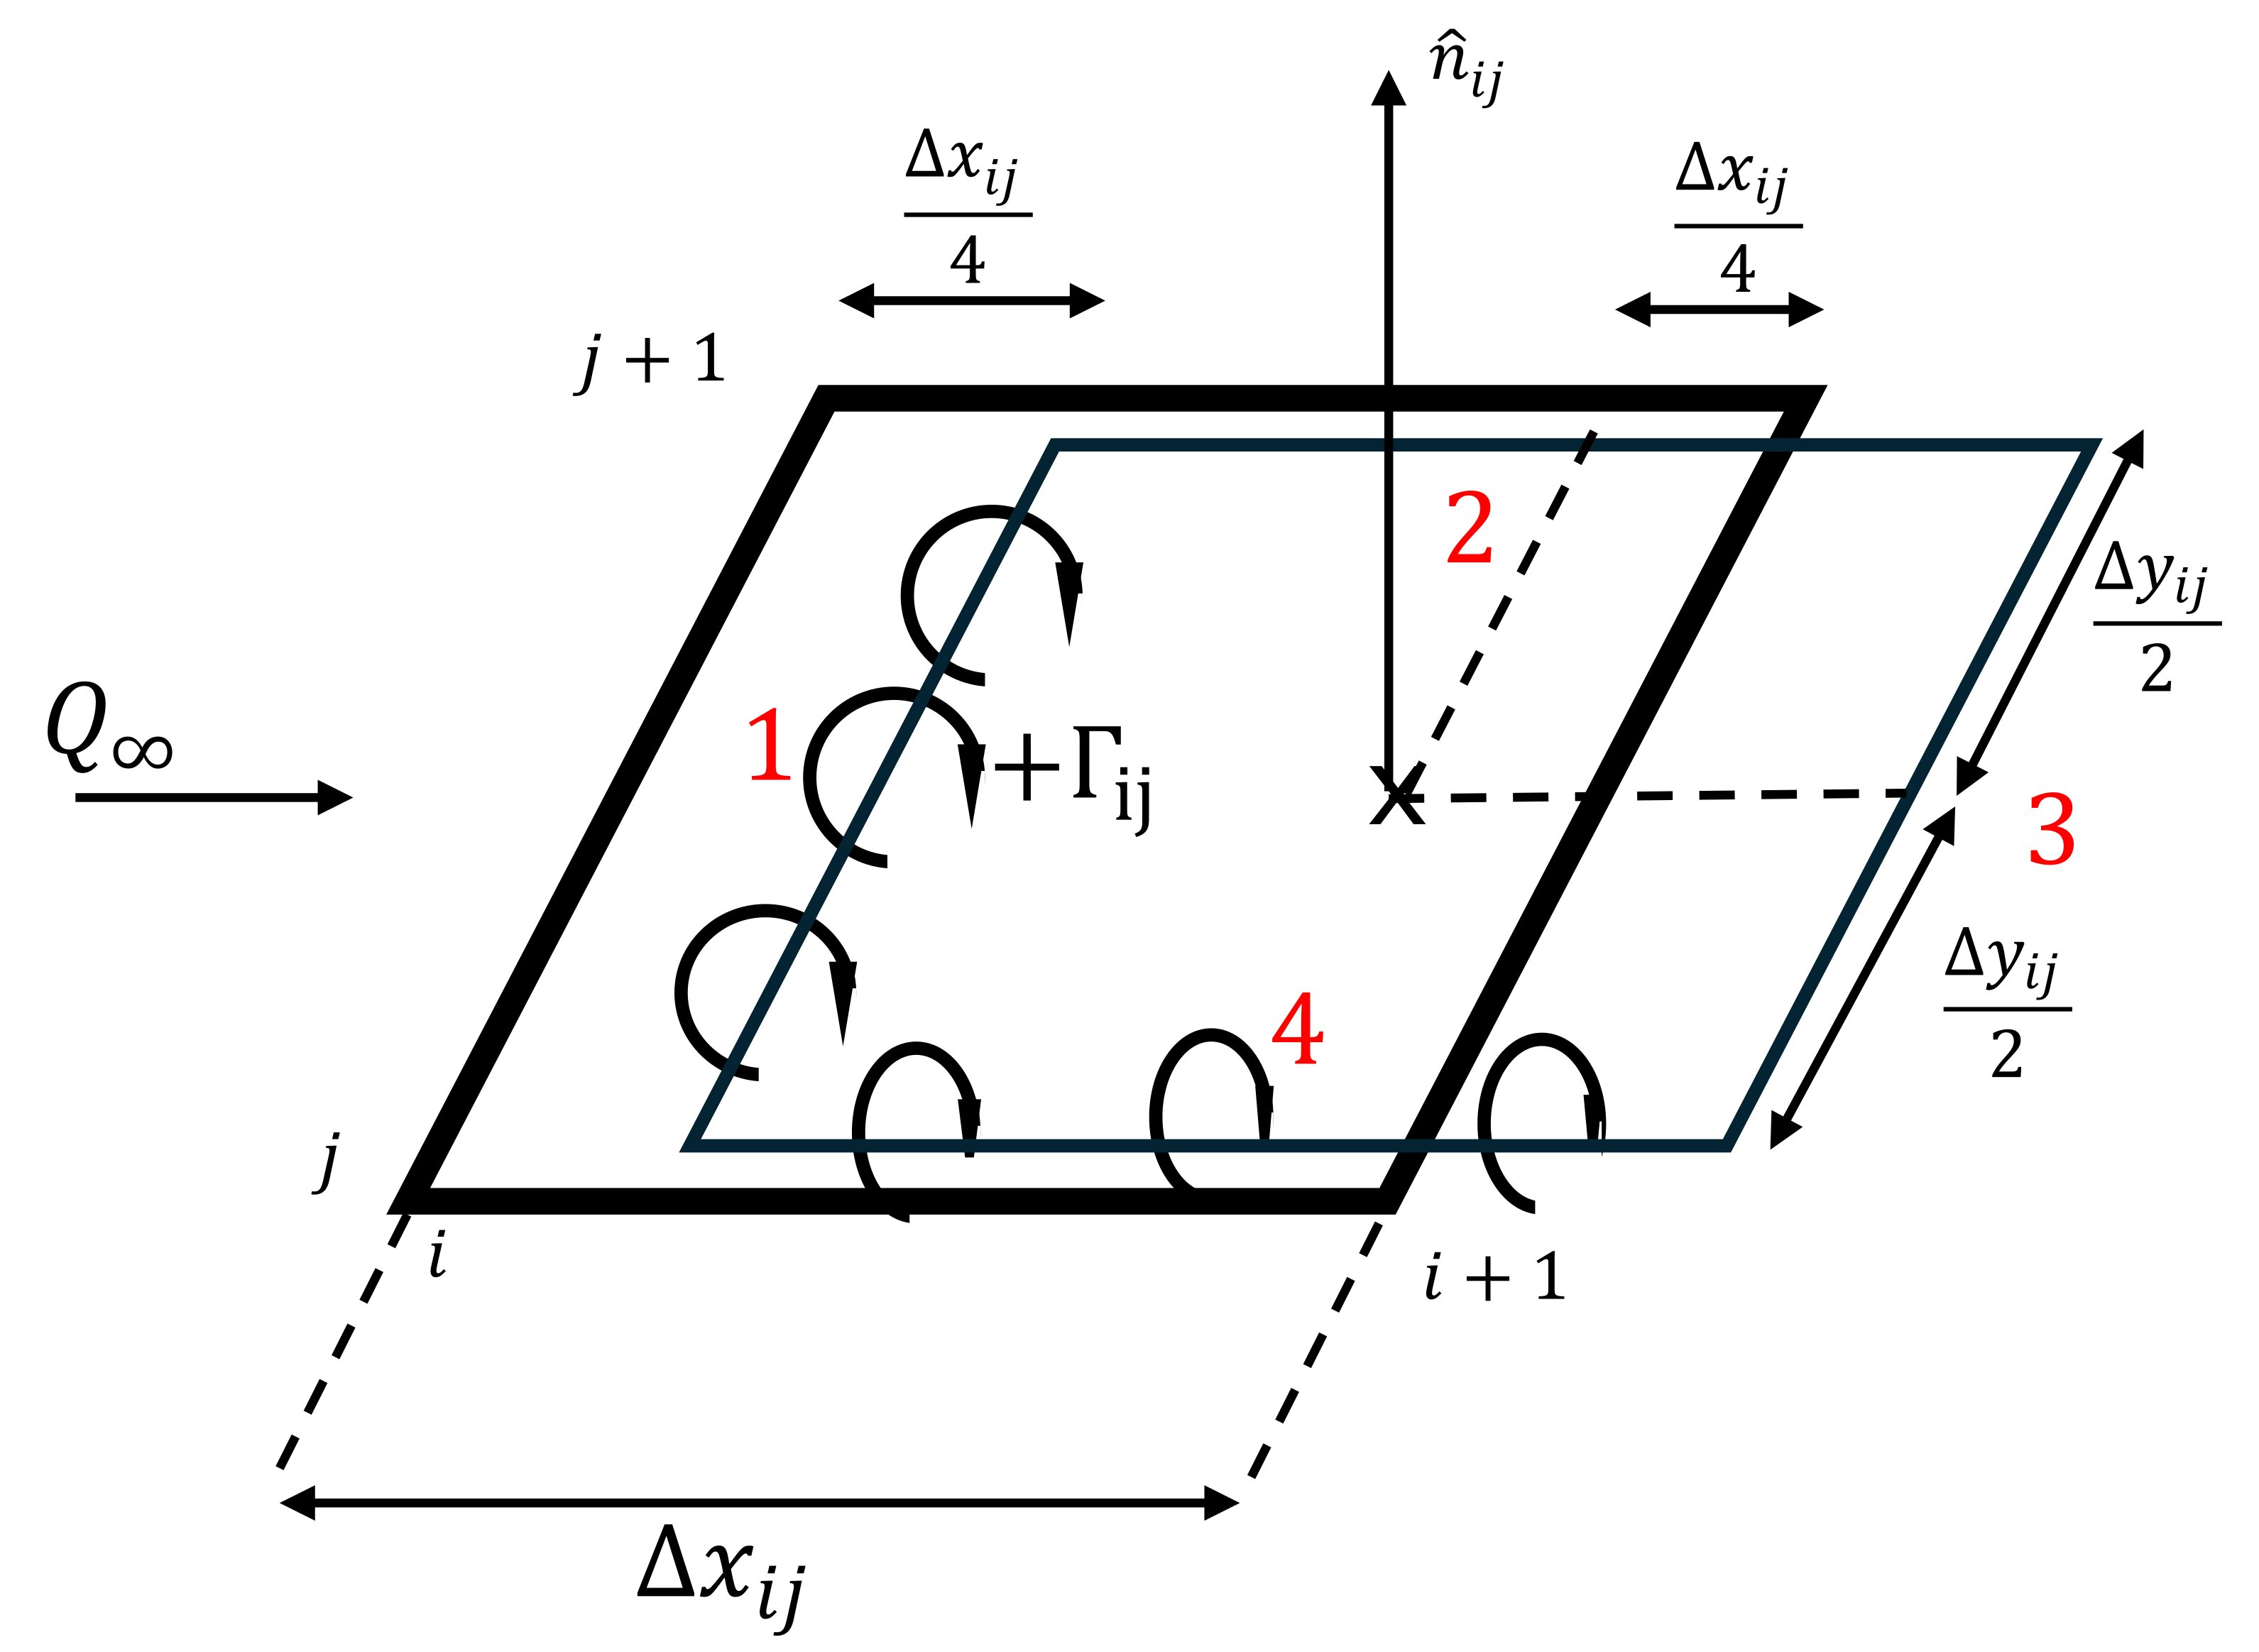
\includegraphics[width=0.8\textwidth]{Quadrilateral vortex ring element.png}
  \caption{Vortex Ring Element}
  \label{fig:VortexRingElement}
\end{figure}



The numbers 1 through 4 on \autoref{fig:VortexRingElement} Vortex Ring Element represent the
four finite straight vortex segments that make up the element. The
induced velocity of the element can be calculated using equation
\eqref{eq:V12} on each segment separately. For an arbitrary point in space
$P(x,y,z)$ the induced velocity is:

\begin{equation}
{\vec{V}}_{P} = {\vec{V}}_{1} + {\vec{V}}_{2} + {\vec{V}}_{3} + {\vec{V}}_{4}
\end{equation}

Where:

\begin{equation}
    \label{eq:Vi}
{\vec{V}}_{i} = \frac{\Gamma}{4\pi}\ \frac{{\vec{r}}_{i,1} \times {\vec{r}}_{i,2}}{\left| {\vec{r}}_{i,1} \times {\vec{r}}_{i,2} \right|}({\vec{r}}_{i,1} - {\vec{r}}_{i,2}) \cdot \left( \frac{{\vec{r}}_{i,1}}{\left| {\vec{r}}_{i,1} \right|} - \frac{{\vec{r}}_{i,2}}{\left| {\vec{r}}_{i,2} \right|} \right)
\end{equation}

These elements are sorted in a two-dimensional grid to cover the lifting
surface shape. To satisfy the trailing edge condition (Kutta condition)
the trailing vortex of the last panel row must be cancelled. Therefore
the last row of panels as well as all the wake panels have the same
circulation $\Gamma$.

\begin{figure}[H]
    \centering
    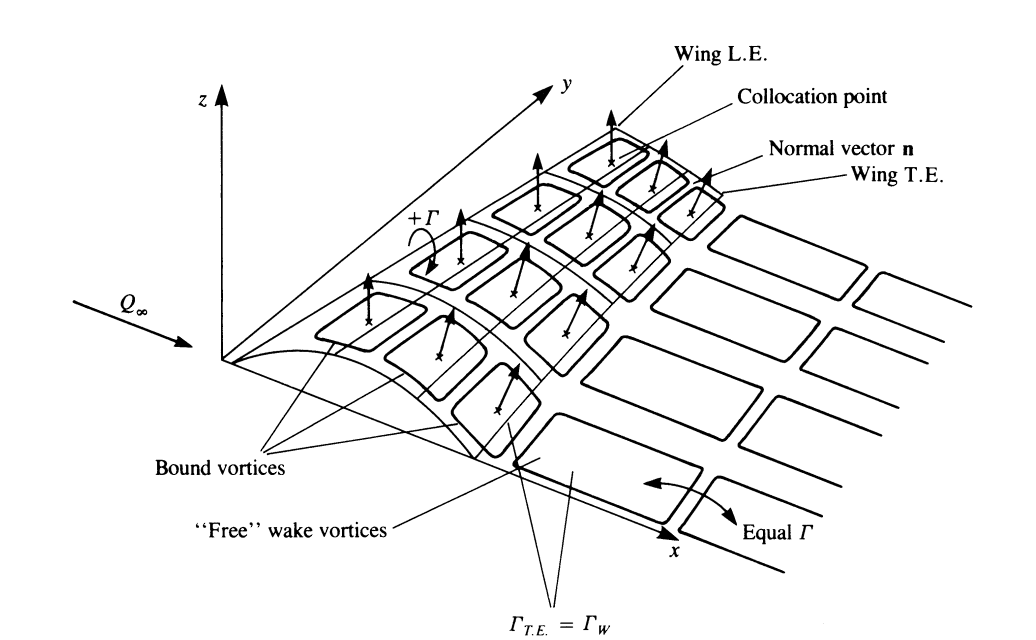
\includegraphics[width=\textwidth]{vortex ring model.png}
    \caption{Vortex ring elements in a grid \cite{katz2001}}
\end{figure}


The influence coefficient $\alpha_{ij}$ is essentially the induced
velocity of the i-th vortex ring element with unitary circulation at the
j-th collocation point. The influence coefficients can easily be
calculated using equation \eqref{eq:Vi}. Iterating over all panels and all
collocation points results in a matrix

\begin{equation}
A = \begin{bmatrix}
a_{11} & a_{12} & \cdots & a_{1m} \\
a_{21} & a_{22} & \cdots & a_{2m} \\
 \vdots & \vdots & \ddots & \vdots \\
a_{m1} & a_{m2} & \cdots & a_{mm}
\end{bmatrix}
\end{equation}

\begin{figure}[H]
  \centering
  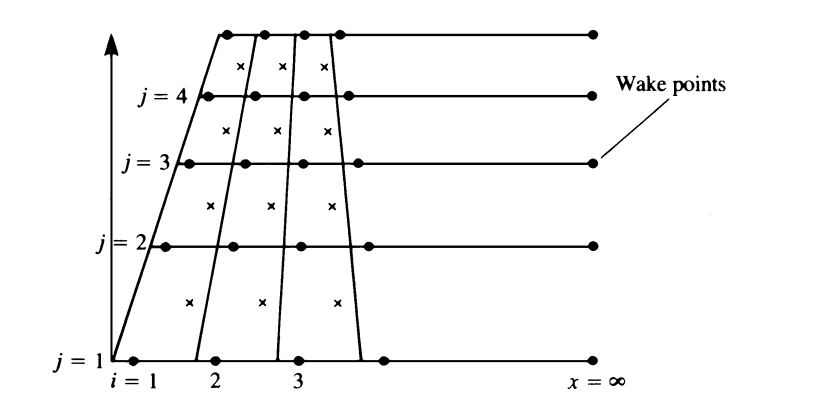
\includegraphics[width=\textwidth]{2D ARRAY OF PANELS.png}
  \caption{Array of wing and wake panel corner points (dots) and of collocation points( $\times$ symbols) \cite{katz2001}}
\end{figure}

For the sake of completeness, the linear set of equations that has to be
solved in order to calculate the circulation intensity of each element
given a certain angle of attack for each panel is:

\begin{equation}
\begin{bmatrix}
a_{11} & a_{12} & \cdots & a_{1m} \\
a_{21} & a_{22} & \cdots & a_{2m} \\
 \vdots & \vdots & \ddots & \vdots \\
a_{m1} & a_{m2} & \cdots & a_{mm}
\end{bmatrix}\begin{bmatrix}
\Gamma_{1} \\
\Gamma_{2} \\
 \vdots \\
\Gamma_{m}
\end{bmatrix} = \begin{bmatrix}
 - {\vec{Q}}_{\infty} \cdot {\hat{n}}_{1} \\
 - {\vec{Q}}_{\infty} \cdot {\hat{n}}_{2} \\
 \vdots \\
 - {\vec{Q}}_{\infty} \cdot {\hat{n}}_{m}
\end{bmatrix}
\end{equation}


The downwash induced at each vortex ring element can be calculated by another set of linear equations

\begin{equation}
\begin{bmatrix}
{w_{ind}}_{1} \\
{w_{ind}}_{2} \\
 \vdots \\
{w_{ind}}_{m}
\end{bmatrix} = \begin{bmatrix}
b_{11} & b_{12} & \cdots & b_{1m} \\
b_{21} & b_{22} & \cdots & b_{2m} \\
 \vdots & \vdots & \ddots & \vdots \\
b_{m1} & b_{m2} & \cdots & b_{mm}
\end{bmatrix}\begin{bmatrix}
\Gamma_{1} \\
\Gamma_{2} \\
 \vdots \\
\Gamma_{m}
\end{bmatrix}
\end{equation}


The lift and drag can then be calculated by using the relationships:

\begin{multline}
    L = \sum_{i = 1}^{M} \sum_{j = 1}^{N} \Delta L_{ij}, \\
    \text{where} \quad \Delta L_{ij} = \begin{cases}
      \rho Q_{\infty} \left( \Gamma_{i,j} - \Gamma_{i - 1,j} \right) \Delta y_{ij}, & \text{for } i > 1 \\
      \rho Q_{\infty} \Gamma_{ij} \Delta y_{ij}, & \text{for } i = 1
    \end{cases}
  \end{multline}

\begin{multline}
D = \sum_{i = 1}^{M} \sum_{j = 1}^{N} \Delta D_{ij}, \\
\text{where} \quad \Delta D_{ij} = \begin{cases}
    \rho w_{\text{ind}_{i,j}} \left( \Gamma_{i,j} - \Gamma_{i - 1,j} \right) \Delta y_{ij}, & \text{for } i > 1 \\
    \rho w_{\text{ind}_{i,j}} \Gamma_{ij} \Delta y_{ij}, & \text{for } i = 1
\end{cases}
\end{multline}


\section{Flutter Analysis Equations}\label{flutter-analysis-equations}

The general form of the aeroelastic equation of motion is \cite{AeroelasticityWright}

\begin{equation}
    \lbrack A\rbrack\ddot{q} + \left( \rho V\lbrack B\rbrack + D \right)\dot{q} + \left( \rho V^{2}\lbrack C\rbrack + \lbrack E\rbrack \right)q = \lbrack 0\rbrack  
\end{equation}



Where:

\begin{itemize}
\item
  $[A]$, $[C]$, and $[E]$, are the structural matrices corresponding to the $[M]$, $[C]$ and
  $[K]$ matrices which is the classical notation used in structural analysis
\item
  $[B]$ and $[C]$ are the aerodynamic matrices which depend on the Mach number
  and the reduced frequency. The way these matrices are computed can
  vary depending on the aerodynamic theory used.
\item
  $q$ are the generalized modal coordinates.
\end{itemize}


\subsection{Interconnection of the Structure with Aerodynamics -- Infinite Plate splines}\label{interconnection-of-the-structure-with-aerodynamics-infinite-plate-splines}

The structural and aerodynamic degrees of freedom are connected by
interpolation. This allows the independent selection of grid points
(nodes) of the structural and aerodynamic matrices thus decoupling the
two discretizations of geometry. This interpolation method is called
splining. The Infinite plate spline which is used here is based on the
structural deformation of a theoretically infinite plate subject to
point loads at given points. The splines are used for two distinct
purposed: as a force interpolator to compute the structurally equivalent
force distribution on the structure given a force distribution on the
aerodynamic mesh and as a displacement interpolator to compute a set of
aerodynamic displacements given as a set of structural displacements.
Mathematically this means that:

\begin{equation}
F_{s} = \left\lbrack G_{s \rightarrow a} \right\rbrack F_{a},\ \ U_{a} = {\lbrack G}_{a \rightarrow s}\rbrack U_{s}
\end{equation}


Where:

\begin{itemize}
\item
  $F_{s}$ and $F_{a}$ are the structural and aerodynamic force
  vectors
\item
  $U_{a}$ and $U_{s}$ are the aerodynamic and structural
  displacement vectors
\item
  $G_{s \rightarrow a}$ and $G_{a \rightarrow s}$ are the spline
  matrices connecting the structural to aerodynamic and vice versa. It
  has been proven by the virtual work principle that the two spline
  matrices are the transform of one another i.e.
  $\left\lbrack G_{s \rightarrow a} \right\rbrack = {{\lbrack G}_{a \rightarrow s}\rbrack}^{T}$
\end{itemize}

\begin{figure}[H]
  \centering
  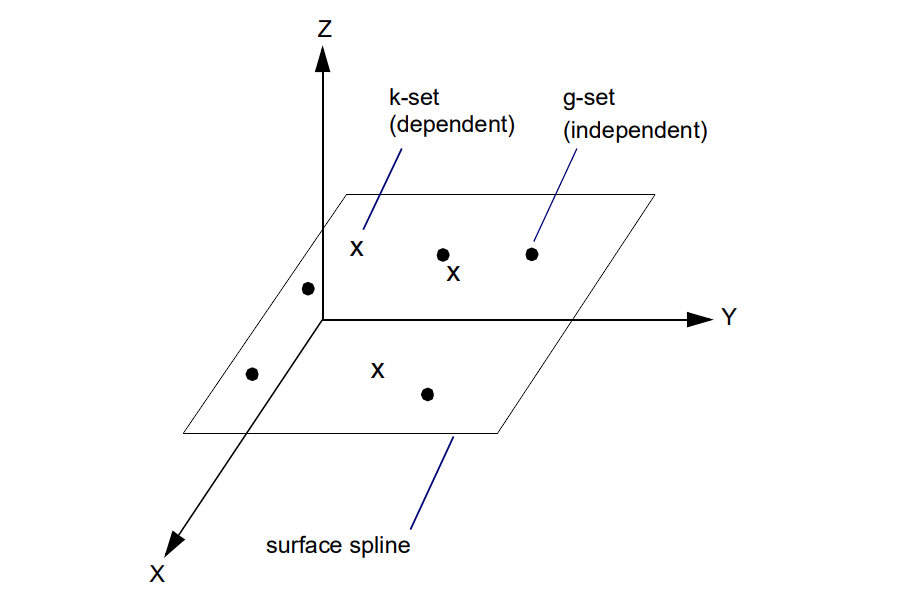
\includegraphics[width=0.9\textwidth]{surface spline.png}
  \caption{Surface Spline coordinate system \cite{msc2021}}
\end{figure}

The Infinite plate spline and all other surface splines are used to find
a surface in the form $w(x,y)$ for all points $(x,y)$ when w is
known at a discrete set of points
$w_{i} = w\left( x_{i},y_{i} \right)$.

The Infinite plate spline mimics the behavior of an infinite plate under
point load. The deflection of such a plate due to a single concentrated
load at $\left( x_{i} = 0,\ y_{i} = 0 \right)$ is called the
fundamental solution. The governing equation is:



\begin{equation}
D\nabla^{4}(w) = D\frac{1}{r}\frac{d}{dr}\left\{ r\frac{d}{dr}\left\lbrack \frac{1}{r}\frac{d}{dr}\left( r\frac{dw}{dr} \right) \right\rbrack \right\} = q
\label{eq:splineequation}
\end{equation}



The general solution to the homogeneous form of \autoref{eq:splineequation} is:

\begin{equation}
w = C_{1} + C_{1}r^{2} + C_{2}\ln(r) + C_{3}r^{2}\ln(r)
\end{equation}

Setting $C_{2} = \ 0\ $to keep the solution finite at $r = 0$ then
integrating from $r = 0$ to $r = \epsilon\ (small\ number)$ leads to
$C_{3} = \frac{P}{8\pi D}$. Thus, the fundamental solution for a
concentrated load is:

\begin{equation}
w = A + Br^{2} + \frac{P}{16\pi D}r^{2}\ln\left( r^{2} \right)
\end{equation}


The fundamental solution can be superimposed to solve the entire plate
problem:

\begin{equation}
w(x,y) = \alpha_{0} + \alpha_{1}x + \alpha_{2}y + \sum_{i = 1}^{N}{K_{i}(x,y)P_{i}}
\end{equation}


Where:

\begin{itemize}
\item
  $K_{i}(x,y) = \frac{1}{16\pi D}r_{i}^{2}\ln\left( r_{i}^{2} \right)$
\item
  $r_{i}^{2} = \left( x - x_{i} \right)^{2} + \left( y - y_{i} \right)^{2}$
\item
  $P_{i}$ concentrated load at $\left( x_{i},y_{i} \right)$
\end{itemize}

The $N+3$ unknowns of are determined from the $N+3$ equations

\begin{equation}
\sum_{}^{}{Pi} = 0
\end{equation}

\begin{equation}
  \sum_{}^{}{x_{i}P_{i}} = 0
\end{equation}

\begin{equation}
  \sum_{}^{}{y_{i}P_{i}} = 0
\end{equation}

\begin{equation}
  w_{j} = a_{0} + a_{1}x_{j} + a_{2}y_{2} + \sum_{i = 1}^{N}K_{ij}P_{i},\ \ (\ j = 1,\ldots,\ N)  
\end{equation}

Where $K_{ij} = K_{i}\left( x_{j},y_{j} \right)$ and
$K_{ij} = K_{ji},\ \ K_{ij} = 0\ when\ i = j$

These $N+3$ equations can be expressed into a matrix form:

\begin{equation}
\begin{bmatrix}
  \begin{array}{c}
    0 \\
    0 \\
    0 \\
    \hline
    w_{1} \\
    w_{2} \\
     \vdots \\
    w_{N}        
  \end{array}
\end{bmatrix} = \begin{bmatrix}
\begin{array}{cccccc}
  0 & 0 & 0 & 1 & \cdots & 1 \\
0 & 0 & 0 & x_{1} & \cdots & x_{N} \\
0 & 0 & 0 & y_{1} & \cdots & y_{N} \\
\hline 
1 & x_{1} & y_{1} & 0 & \cdots & K_{1N} \\
1 & x_{2} & y_{2} & K_{21} & \cdots & K_{2N} \\
 \vdots & \vdots & \vdots & \vdots & \cdots & \vdots \\
1 & x_{N} & y_{N} & K_{N1} & \cdots & 0
\end{array}
\end{bmatrix}
\begin{bmatrix}
  \begin{array}{c}
    a_{0} \\
    a_{1} \\
    a_{2} \\
    \hline
    P_{1} \\
    P_{2} \\
     \vdots \\
    P_{N}
        
  \end{array}
\end{bmatrix} = \lbrack C\rbrack\lbrack P\rbrack
\end{equation}



Now that the $a_{i}$ and $P_{i}$ any quantity can be interpolated at
any point in the $(x,y)$ plane using the following matrix equation:

\begin{equation}
\left\{ w \right\} = \begin{bmatrix}
1 & x_{1} & y_{1} & K_{1,1} & K_{1,2} & \cdots & K_{1,n} \\
1 & x_{2} & y_{2} & K_{2,1} & K_{2,2} & \cdots & K_{2.m} \\
 \vdots & \vdots & \vdots & \vdots & \vdots & \cdots & \vdots \\
1 & x_{n} & y_{n} & K_{n,1}\  & K_{n,2} & \cdots & K_{n,n}\ 
\end{bmatrix} \cdot \lbrack C\rbrack^{- 1}\begin{bmatrix}
0 \\
0 \\
0 \\
w_{1} \\
w_{2} \\
 \vdots \\
w_{N}
\end{bmatrix}
\end{equation}

\subsection{The PK Method of Flutter Solution}
\label{the-pk-method-of-flutter-solution}

The fundamental equation for modal flutter analysis by the PK method is \cite{msc2021}:

\begin{equation}
\left\lbrack M_{hh}p^{2} + \left( B_{hh} - \frac{1}{4}\rho cV\frac{Q_{hh}^{I}}{k} \right)p + \left( K_{hh} - \frac{1}{2}\rho V^{2}Q_{hh}^{R} \right)\  \right\rbrack \cdot \left\{ u_{h} \right\} = \underline{0}
\end{equation}


Where:

\begin{itemize}
\item
  $M_{hh} =$ modal mass matrix, usually diagonal
\item
  $B_{hh} =$ modal damping matrix
\item
  $K_{hh} =$ modal stiffness matrix, usually diagonal, may be complex
  if actual damping is used
\item
  $Q_{hh}(M,k) =$ aerodynamic force matrix which is a function of mach
  number and reduced frequency $k = \frac{\omega\overline{c}}{2V}$
\item
  $Q_{hh}^{R},\ Q_{hh}^{I}$ are the real and imaginary parts of the
  aerodynamic force matrix $Q_{hh}$ also called aerodynamic stiffness
  and aerodynamic damping matrices respectively
\item
  $k = \frac{\omega\overline{c}}{2V}$ reduced frequency
\item
  $M =$ Mach number
\item
  $V = \ $Velocity
\item
  $\rho =$ fluid density
\item
  $\left\{ u_{h} \right\} =$ modal amplitude vector (modal
  participation vector)
\item
  $p = \omega(\gamma \pm i)$ eigenvalue
\end{itemize}


The equation is rewritten in the state-space form with order reduction

\begin{equation}
    \label{eq:PKss}
\lbrack A - pI\rbrack\left\{ {\overline{u}}_{h} \right\} = 0
\end{equation}

Where:

\begin{equation}
\lbrack A\rbrack = - \begin{bmatrix}
\mathbf{\lbrack 0\rbrack} & \mathbf{\lbrack I\rbrack} \\
 - M_{hh}^{- 1}\left( K_{hh} - \frac{1}{2}\rho V^{2}Q_{hh}^{R} \right) & - M_{hh}^{- 1}\left( B_{hh} - \frac{1}{4}\rho cV\frac{Q_{hh}^{I}}{k} \right)
\end{bmatrix}
\end{equation}

\begin{equation}
  {\overline{u}}_{h} = \begin{bmatrix}
    u_{h} \\
    {\dot{u}}_{h}
    \end{bmatrix}\  
\end{equation}


The basic algorithm for the pk method involves the following steps:

\begin{enumerate}
\def\labelenumi{\arabic{enumi}.}
\item
  Make an initial guess of the frequency for the mode
\item
  Calculate the corresponding reduced frequency $k$ and airspeed $V$
\item
  Determine (by interpolation) the aerodynamic stiffness and damping
  matrices $Q_{hh}^{R},\ Q_{hh}^{I}$
\item
  Determine the frequencies for the system at this flight condition
  using Equation \eqref{eq:PKss}
\item
  Take the frequency solution that was closest to the initial guess and
  repeat steps 1-5 until the frequency converges
\item
  Store the final modal frequency and modal damping
\item
  Consider the next mode of interest using the same procedure until all
  modes of interest have been investigated
\end{enumerate}


\section{Optimization techniques }
\label{optimization-techniques}

\subsection{Brent's -- Dekker Line search method }
\label{brents-dekker-line-search-method}

This algorithm aims to find the minimum of a function of one
variable without using its derivatives. This algorithm is commonly used
when finding the minimum of a function $g\left( \mathbf{x} \right)$ of
several variables \cite{brent1973}. To this end the following function often needs to be
minimized

\begin{equation}
    \label{eq:minfun}
\gamma(\lambda) = f(\mathbf{x}_{0} + \lambda\mathbf{s})
\end{equation}

where $\mathbf{x}_{0}$ and $\mathbf{s}$ are fixed and $\lambda$ is
a scalar variable. This problem essentially describes a one-dimensional
search beginning form $\mathbf{x}_{0}$ in the direction of
$\mathbf{s}$.

The algorithm finds an approximation to the minimum of a function $f$
defined on the interval $\lbrack a,\ b\rbrack$. There are six
significant points $a,b,u,v,w\ and\ x$ not all distinct. These points
are initialized as follows:

\begin{equation}
    \label{eq:brentspoints}
v = w = x = a + \left( \frac{3 - \sqrt{5}}{2} \right)(b - a)
\end{equation}

The number $\left( \frac{3 - \sqrt{5}}{2} \right)$ comes from the
golden section search algorithm and is somewhat arbitrary. The points
defined in \eqref{eq:brentspoints} serve a specific purpose:


\begin{itemize}
\item
  Points $a$ and $b$ define the interval within which a local
  minimum lies
\item
  $x$: of all the points at which $f$ has been evaluated, $x$ is
  the one with the least value of $f$
\item
  $w$ is the point with the next lowest value of $f$
\item
  $v$ is the previous value of $w$
\item
  $u$ is the last point at which f has been evaluated
\end{itemize}

\begin{figure}
  \centering
  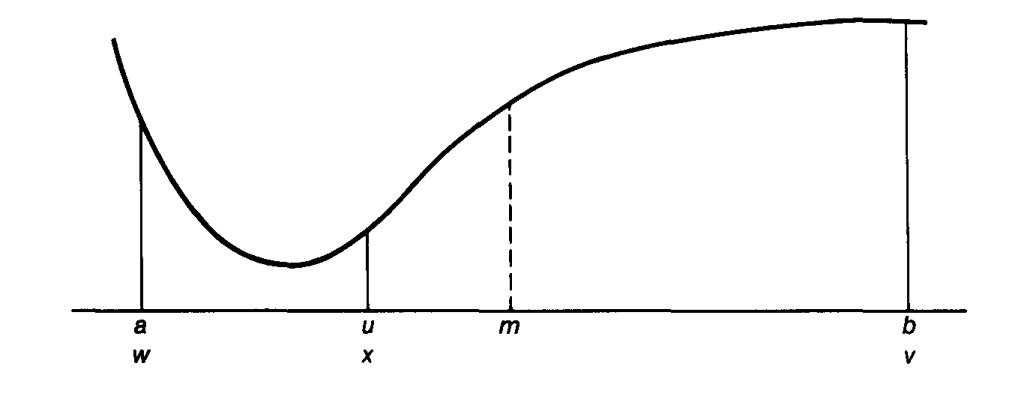
\includegraphics[width=\textwidth]{brents_six_points.png}
  \caption{A possible configuration of points \cite{brent1973} }
\end{figure}

A typical iteration of the algorithm evolves as follows:


\begin{enumerate}
\def\labelenumi{\arabic{enumi}.}
\item
  Let $m = 1\text{/}2(a + b)$ be the midpoint of the interval

  \begin{enumerate}
  \def\labelenumii{\alph{enumii}.}
  \item
    If $|x - m| \leq 2 \cdot tol - \frac{1}{2}(b - a)\ $then the
    algorithm terminates with x as the minimum
  \item
    Otherwise, the numbers $p$ and $q$ are calculated such that
    $x + p/q$ is the minimum of the parabola passing through
    points\\
    $\left( v,f(v) \right),\ \ \left( w,f(w) \right),\ \ \left( x,f(x) \right)$
  \end{enumerate}
\item
  Let $e$ be the value of $p/q$

  \begin{enumerate}
  \def\labelenumii{\alph{enumii}.}
  \item
    If $|e| \leq tol$,
    $q = 0$,$x + p\text{/}q \notin \lbrack a,b\rbrack$ or
    $\left| p\text{/}q \right| \geq 1/2|e|$ then the golden ration
    step is performed:
  



\begin{equation}
  u =
  \begin{cases} 
  \frac{\sqrt{5} - 1}{2}x + \frac{3 - \sqrt{5}}{2}a, & \text{if } x \geq m \\ 
  \frac{\sqrt{5} - 1}{2}x + \frac{3 - \sqrt{5}}{2}b, & \text{if } x < m
  \end{cases}
\end{equation}

\item
  Otherwise $u = x + p\text{/}q$ (the
  distances$|u - x|,\ \ u - a,\ \ b - u\ $must be at least $tol$)
\end{enumerate}
\end{enumerate}


\begin{enumerate}
\def\labelenumi{\arabic{enumi}.}
\setcounter{enumi}{2}
\item
  $f$ is evaluated at the new point $u$ the points
  $a,b,v,w\ and\ x$ are updated and the cucle repeats
\end{enumerate}

The algorithm typically terminates when $x = b - tol$ or
$x = a + tol$ after a parabolic interpolation has been performed where
the condition that $|u - x| \geq tol$ has been enforced. The next
parabolic interpolation point lies close to x and b so u is forced to be
$x - tol$.

\begin{figure}[H]
    \centering
    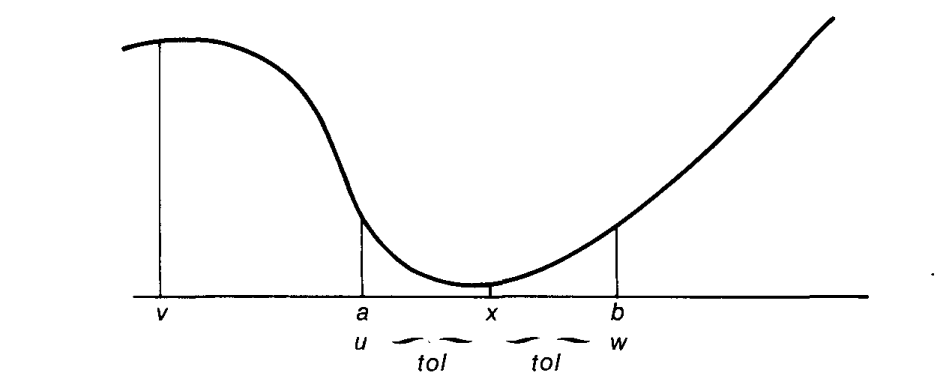
\includegraphics[width=\textwidth]{brents algorithm termination configuration.png}
    \caption{typical terminal configuration of important points \cite{brent1973}}
\end{figure}

\subsection{Powell's Method}
\label{powells-method}

Powell's method is a modified cyclic coordinate search. Both methods aim
to minimize a multivariate function without using any of its
derivatives. That's why they are called zero-order methods.

The Cyclic coordinate search method is in essence a series of
line-search optimizations performed cyclically over all inputs of the
function. The search starts from an initial $x^{(0)}$ and optimizes
the first input:

\begin{equation}
\mathbf{x}^{(1)} = \arg_{x_{1}}{\min{f\left( x_{1},x_{2}^{(0)},\ldots,x_{n}^{(0)} \right)}}
\end{equation}

Having solved this, it optimizes the next coordinate:

\begin{equation}
\mathbf{x}^{(2)} = \arg_{x_{2}}{\min{f\left( x_{1}^{(1)},x_{2},\ldots,x_{n}^{(1)} \right)}}
\end{equation}

This can also be expressed with the help of equation \eqref{eq:minfun} if
$\mathbf{s}$ is the i\textsuperscript{th} basis vector for
$i = 1,\ldots,n$

Any line search algorithm can be used but Brent's Algorithm has seen
wide usage in optimization libraries including SciPy's implementation of
the Powell method.

\begin{figure}[H]
    \centering
    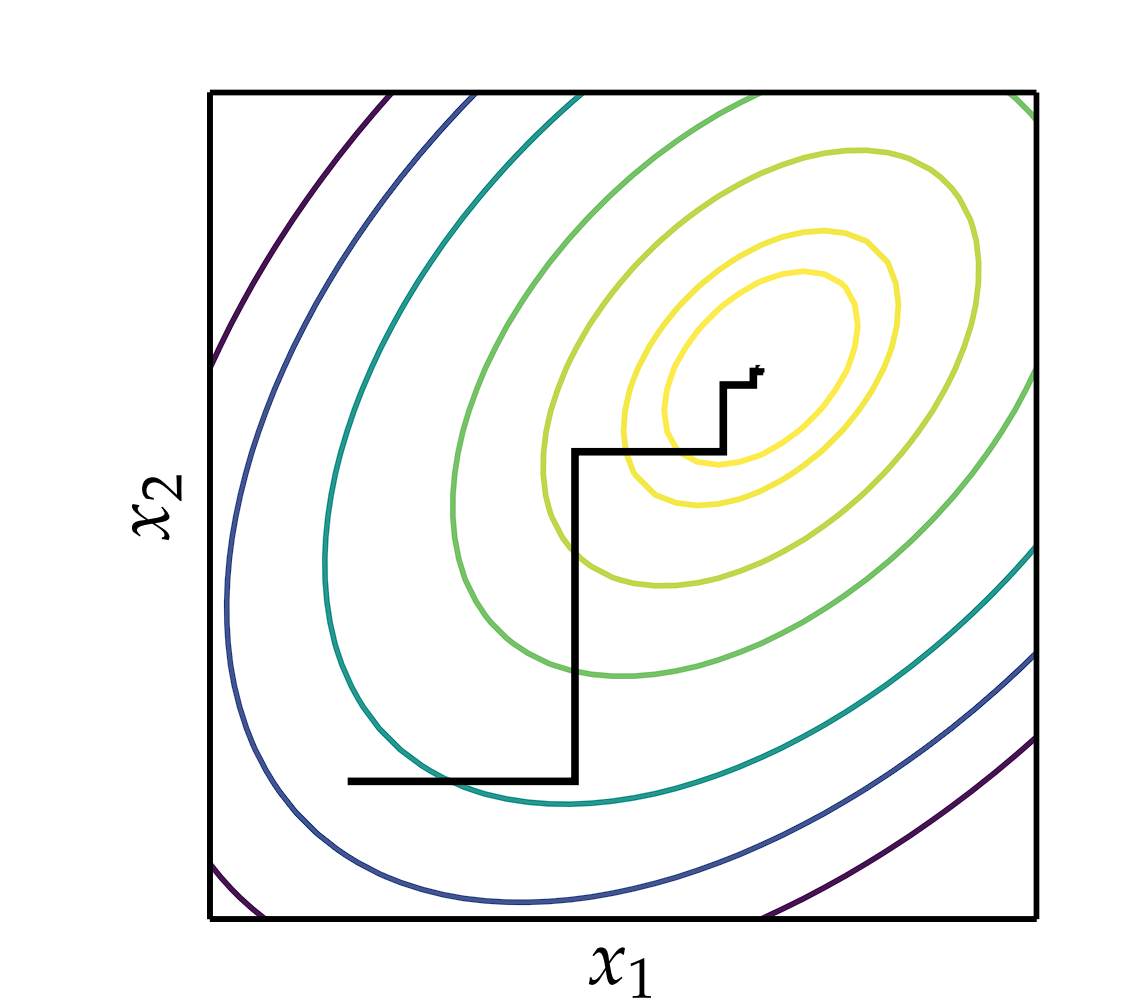
\includegraphics[width=0.5\textwidth]{cyclic coordinate search.png}
    \caption{Cyclic coordinate search \cite{kochenderfer2019}}
    \label{fig:CCsearch}
\end{figure}

As can be seen in \autoref{fig:CCsearch} a weakness of this method is the slow
traversal of diagonal valleys where repeated small steps are taken in
every direction. M.J.D. Powell's idea was to expand the cyclic
coordinate search method so that it can search in directions that are
not orthogonal to each other and are also not the basis vectors. In
order to achieve this new capability, Powell's algorithm maintains a list
of search directions
$\left\lbrack \mathbf{u}^{(0)},\ldots\mathbf{u}^{(n)} \right\rbrack$
which are initially the coordinate basis vectors
$\mathbf{u}^{(i)}=\mathbf{e}^{\left( \mathbf{i} \right)}$ for
all $i$.

Starting at $\mathbf{x}^{(0)}$ Powell's method conducts a line search
as before for each search direction in succession:


\begin{equation}
\mathbf{x}^{(i + 1)} \leftarrow linesearch\left( f,\mathbf{x}^{(i)}\mathbf{,}\mathbf{u}^{(i)} \right)\mathbf{\ }for\ i\ in\ \lbrack 0,\ldots,n\rbrack
\end{equation}

Next the all the search directions are shifted down by one index
dropping the oldest search direction,$\mathbf{u}^{(0)}\ $

\begin{equation}
\mathbf{u}^{(i)} \leftarrow \mathbf{u}^{(i + 1)}\ for\ i\ in\ \lbrack 0,\ldots,n - 1\rbrack
\end{equation}

The last search direction is replaced with the direction from
$\mathbf{x}^{(0)}$ to $\mathbf{x}^{(n + 1)}$, which is the overall
direction of progress over the last n line searches:

\begin{equation}
\mathbf{u}^{(n)} \leftarrow \mathbf{x}^{(n + 1)} - \mathbf{x}^{(0)}
\end{equation}

This process is repeated until convergence.
\begin{figure}[H]
    \centering
    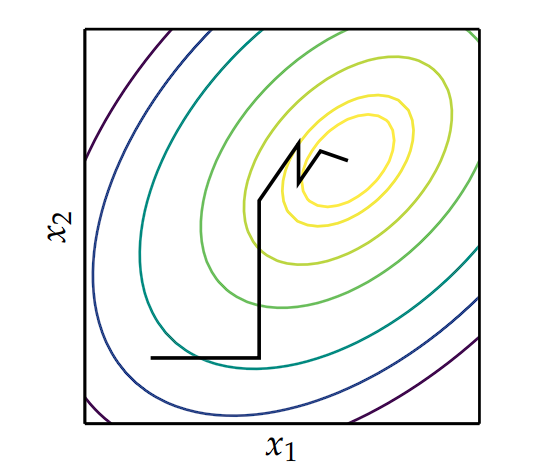
\includegraphics[width=0.5\textwidth]{powells method.png}
    \caption{Powell's method \cite{kochenderfer2019}}
    \label{fig:Powell}

\end{figure}

As can be seen in \autoref{fig:Powell} Powell's method begins the same as cyclic
coordinate search but gradually learns conjugate direction.


\subsection{Genetic Algorithm}
\label{genetic-algorithm}

Genetic algorithms mimic the logic behind Darwinian evolution, where the
fitter individuals are more likely to pass on their genes to the next
generation. The chromosomes of each individual define a single design
point. At each generation the chromosomes of the fitter individuals are
passed on to the next generation after undergoing the genetic operation
of \emph{crossover} and \emph{mutation}

Chromosomes are often represented by a binary array but in this case an
array of real values describes the design space better.

\subsubsection{Initialization}

The Genetic Algorithm begins by initializing a population with random
chromosomes

\subsubsection{Parent Selection}

The selection process is the process of choosing which chromosomes will
be selected to create offsprings for the next generation after being
subjected to the crossover and mutation genetic processes. There are
many methods of selecting which individuals get to mate and combine
their genes, some of the most popular include:

\begin{itemize}
\item
  Roulette Wheel selection: Where each individual is assigned an area of
  an imaginary roulette proportional to their fitness. Then the roulette
  is spun until the desired number of parents is reached. This method is
  simple and effective in most cases. It can become overwhelmed by
  individuals who are much fitter than the rest of the population
\item
  Tournament selection: A subset of individuals is selected at random
  and then the best from this subject is selected as a parent. The
  process is repeated until the desired number of parents is reached
\item
  Steady state Selection: A steady portion of the population is replaced
  at each generation. Only the weakest individuals are replaced by
  offsprings, this method insures that the fittest individual is
  maintained most of the time. A disadvantage of this method is that it
  is slow to adapt as only a small portion of the population is replaced
  at every generation
\end{itemize}

\subsubsection{Crossover}

Crossover is the way the chromosomes of the parents are combined to
create an offspring. There are several crossover schemes. The most
commonly used are :
\begin{samepage}
\begin{itemize}
\item
  Single point crossover

In this scheme the first portion of parent A forms the first portion for the child chromosome and the latter portion of parent B's chromosome
forms the latter part of the child chromosome.

\begin{figure}[H]
    \centering
    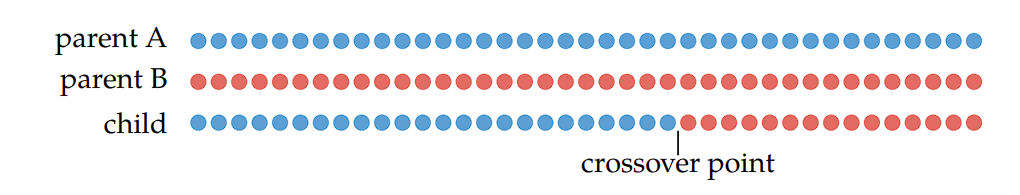
\includegraphics[width=\textwidth]{single point crossover.png}
    \caption{Single Point Crossover \cite{kochenderfer2019}}

\end{figure}


\item
  Two-point crossover


Same as before but a second crossover point is added.

\begin{figure}[H]
    \centering
    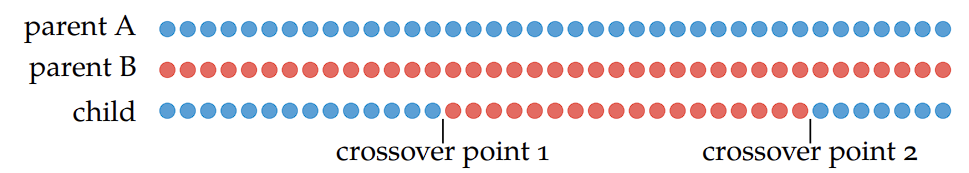
\includegraphics[width=\textwidth]{two point crossover.png}
    \caption{Two-point Crossover \cite{kochenderfer2019}}

\end{figure}

\item
  Uniform crossover


In this scheme every chromosome has a 50\% chance of coming from parent
A or parent B.
\begin{figure}[H]
    \centering
    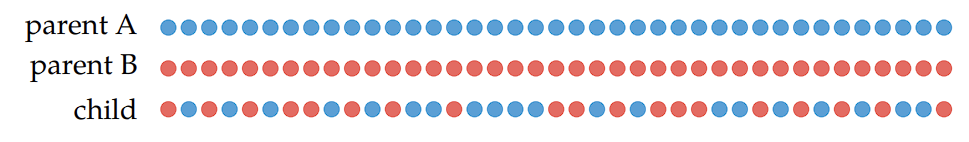
\includegraphics[width=\textwidth]{uniform crossover.png}
    \caption{Uniform Crossover \cite{kochenderfer2019}}

\end{figure}
\end{itemize}
\end{samepage}

\subsubsection{Mutation}

Mutation is a necessary step of the genetic algorithm since it allows new traits to develop which were not present in the initial population. In essence a random value is added to a random chromosome of a randomly selected offspring. The chance of a mutation occurring to an individual is called the \emph{mutation rate}

\subsubsection{Elitism}

Elitism is a strategy that ensures that a fixed number of the most fit
individuals survive to the next generation

Genetic algorithms have a very wide spectrum of application and are very adaptable to many problems. But there is a catch. All those parameters and strategies affect the results greatly and there exists no standard method of selecting every parameter. So, it is the responsibility of the researcher to understand the problem at hand and through experimentation and model hyperparameter tuning techniques determine a
good enough set of parameters.

\subsection{Neural Networks}
\label{neural-networks}

\subsubsection{What are Artificial Neural Networks (ANN's)}

An artificial neural network is a computational model which draws inspiration from the way a biological brain works. The basic structure of an ANN consists of interconnected nodes (or neurons) organized in layers.

The base unit of this structure is a neuron. A neuron has a very simple structure. It accepts an arbitrary number of inputs along with a bias and only has one output. The output can be binary or scalar. Within the neuron a summation is performed using the weight of each input and the bias. The result of each summation is further processed through an ``activation function'' and the output is reached. The activation function allows for nonlinear behavior of the neural networks. It can be
any function, but some functions have prevailed.

\begin{figure}[H]
    \centering
    \includesvg[width=\textwidth]{Neuron.svg}
    \caption{The Structure of a Neuron}

\end{figure}


The basic architecture of a neural network consists of:

\begin{enumerate}
\def\labelenumi{\arabic{enumi}.}
\item
  An input layer which is responsible for receiving the initial data.
  Each neuron in the input layer depicts a specific feature or attribute
  of the input data
\item
  Hidden layers, which are intermediate layers between the input and
  output layers which are responsible for complex feature recognition.
\item
  The weights and biases which are to be used in the neural network, and
  which are the parameters to be trained in order for the neural network
  to make meaningful predictions.
\item
  An output layer which generates the final predictions. The output can
  be binary for classification problems or scalar for regression
  problems.
\end{enumerate}

\begin{figure}[H]
    \centering
    \includesvg[width=\textwidth]{Neural Network.svg}
    \caption{Structure of a Neural Network \cite{takyar2025}}

\end{figure}

The number of Hidden layers in a neural network can vary. Neural
networks which do not have any hidden layers are called ``shallow'', on
the other hand Neural Networks with hidden layers are called Deep Neural
Networks.

\subsubsection{Artificial Neural Network Training}

As stated previously, for a neural network to be useful it has to be trained. Training involves gathering data similar to the ones that the NN is supposed to predict and then performing an optimization of the weights and biases within this network to minimize some loss function. A loss function is a measure of the amount of error. There are many loss functions commonly used for Neural networks, but when a Neural network
is trained on a regression problem the loss function is usually one of the following:

\begin{enumerate}
\def\labelenumi{\arabic{enumi}.}
\item
  Mean Squared Error (MSE)
\end{enumerate}

\begin{equation}
MSE = \frac{1}{N}\sum_{i = 1}^{N}\left( y_{i} - \hat{y} \right)^{2}
\end{equation}

\begin{enumerate}
\def\labelenumi{\arabic{enumi}.}
\setcounter{enumi}{1}
\item
  Root Mean Squared Error
\end{enumerate}

\begin{equation}
RMSE = \ \sqrt{MSE} = \sqrt{\frac{1}{N}\sum_{i = 1}^{N}\left( y_{i} - \hat{y} \right)^{2}}
\end{equation}

\begin{enumerate}
\def\labelenumi{\arabic{enumi}.}
\setcounter{enumi}{2}
\item
  Mean Average Error (MAE)
\end{enumerate}

\begin{equation}
MAE = \frac{1}{N}\sum_{i = 1}^{N}{|y_{i} - \hat{y}|}
\label{eq:MAE}
\end{equation}

Where: $\hat{y}\ is\ the\ predicted\ value\ of\ y$

Minimizing any of these functions on test data that the network hasn't
seen before is the goal of training.

To achieve this goal first the available data which contain both the input and the wanted output, are randomly split between training data (those that will be used for the adjustment of weights and biases) and test data (those which will be used to judge the performance of the neural network). Then through a process called backpropagation (the exact explanation of which is beyond the scope of this thesis) on batches of the training data the weights are updated in such a way so as to reduce the value of the loss function for this particular set of data points. Once all the batches of data have been run through the network and the weights have been adjusted accordingly, we say that the network has completed one pass through the training data This procedure estimates the negative gradient of the loss function and so the network works its way down the slope of the loss function. The number of times this procedure is repeated is called epochs. The number of epochs should be such that an optimum solution is reached without overfitting the network to the test data.

\subsubsection{Hyperparameter Tuning}

As we have seen, in order to define a neural network many parameters have to be chosen in advance. Those parameters include the number of hidden layers, the number of neurons in each layer along with the activation function of each layer to name a few. The best set of parameters is not known a priori and there is no method of selecting the
optimal set.

The process of optimization of a model's hyperparameters is called \emph{hyperparameter tuning}. There are many optimization algorithms that achieve this. One of the more interesting ones and the one that will be employed for this application is the HyperBand algorithm \cite{li2018hyperbandnovelbanditbasedapproach}. The algorithm is an improvement of the Successive Halving
algorithm.

The Idea behind the Successive halving algorithm is quite simple. It uniformly allocates a budget of resources (computational time) to a set of hyperparameters evaluates the performance of each test, reject the bottom 50\% and repeat until one configuration remains. The problem with this algorithm is that it is not known whether testing a larger number of configurations with limited budget each or a smaller number of configurations with more budget will result in a better outcome.

This is the problem that the HyperBand algorithm was made to tackle. It does this by performing a grid search over feasible values of $n$ and $r$, where $n$ is the number of configurations to be tested and $r$ is the minimum resource that is allocated to all configurations before they are allowed to be discarded.
    \chapter{Methodology}
\label{Ch:methodology}
\chapterprecis{
In this chapter the theoretical background developed in \autoref{Ch:Theory}  will
be put to practice to solve an actual example problem. This chapter will
explain the problem that is to be solved. It will explain how the model
is set up for aeroelastic analysis as well as the process used to
optimize the design.}

\section{Problem Introduction }
\label{problem-introduction}

The problem that has been chosen as an example application of all the
theory developed in the previous chapter is the flutter characteristics
study of the ASW 28 glider main wing and the subsequent material design
optimization to tailor the flutter characteristics to specific
requirements. This choice of this specific aircraft is because it has an
extremely large aspect ratio thus making it also very flexible.
Moreover, the main goal of a glider is to achieve the best glide angle
so reduction of weight is of utmost importance and so these vehicles are
ideal for this application as they combine the high likelihood of
flutter occurring with the need to optimize for the lowest weight
possible.

''The ASW 28 is Schleicher's high-performance glider for the
FAI-Standard Class with 15m span.'' \cite{asw28}. The technical data of this
aircraft are summarized in \autoref{fig:TechnicalDataofASW28glider} :

\begin{figure}[H]
\centering
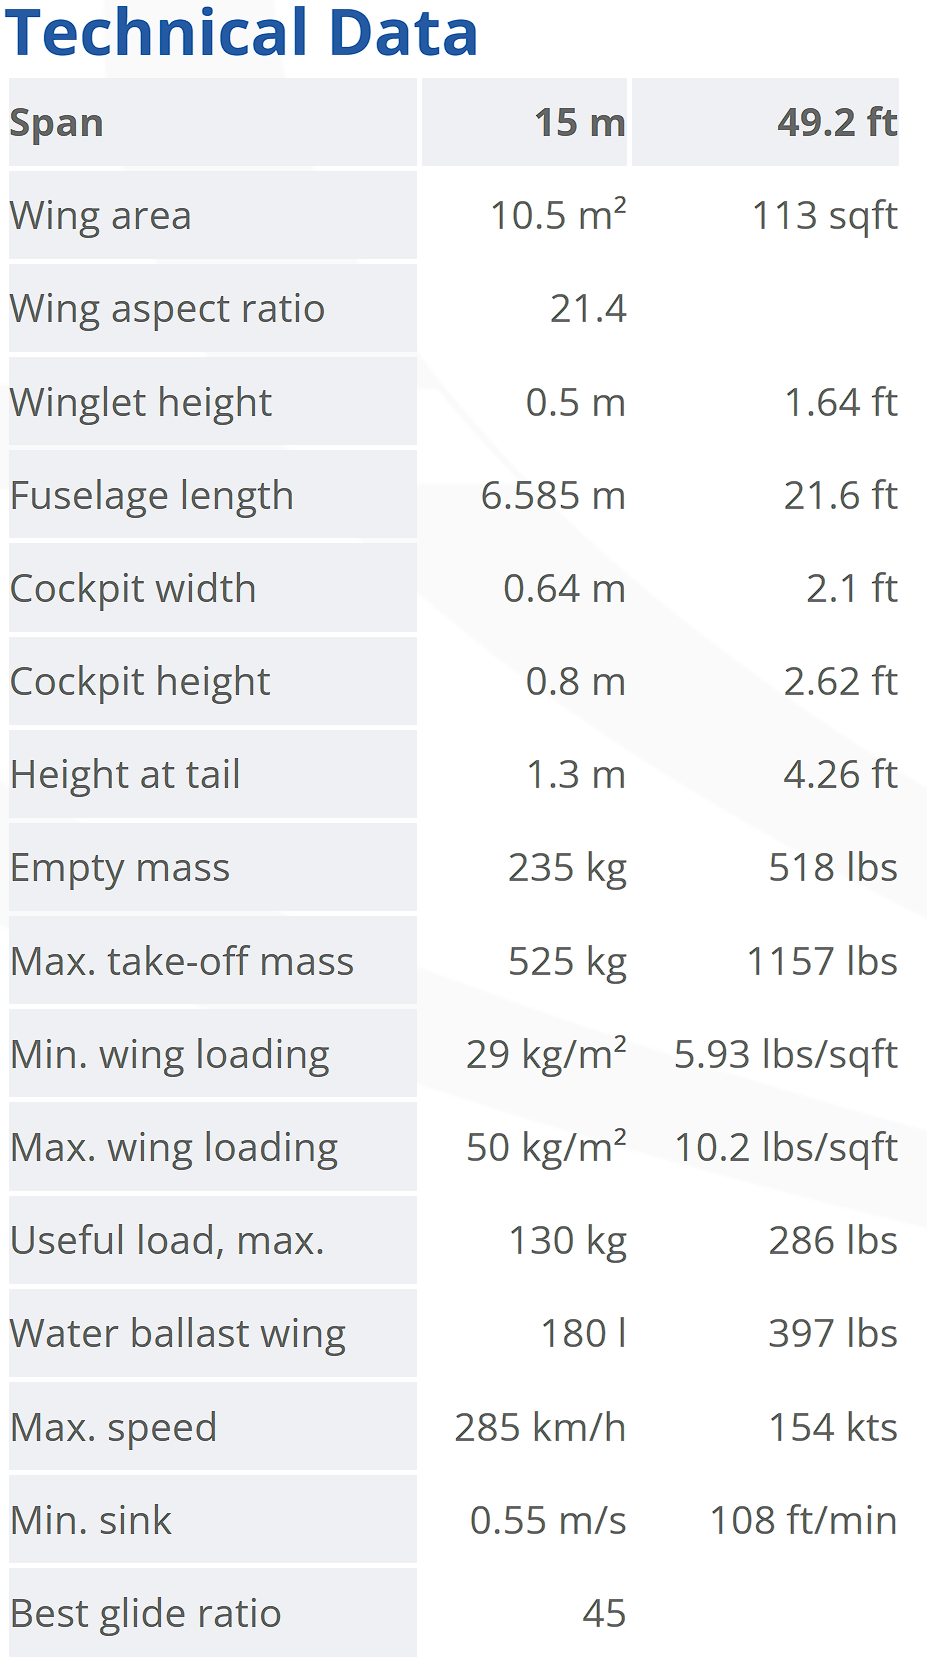
\includegraphics[width=2.92073in]{ASW28_characteristics.png}
\caption{Technical Data of ASW 28 glider \cite{asw28}}
\label{fig:TechnicalDataofASW28glider}
\end{figure}

\begin{figure}[H]
\centering
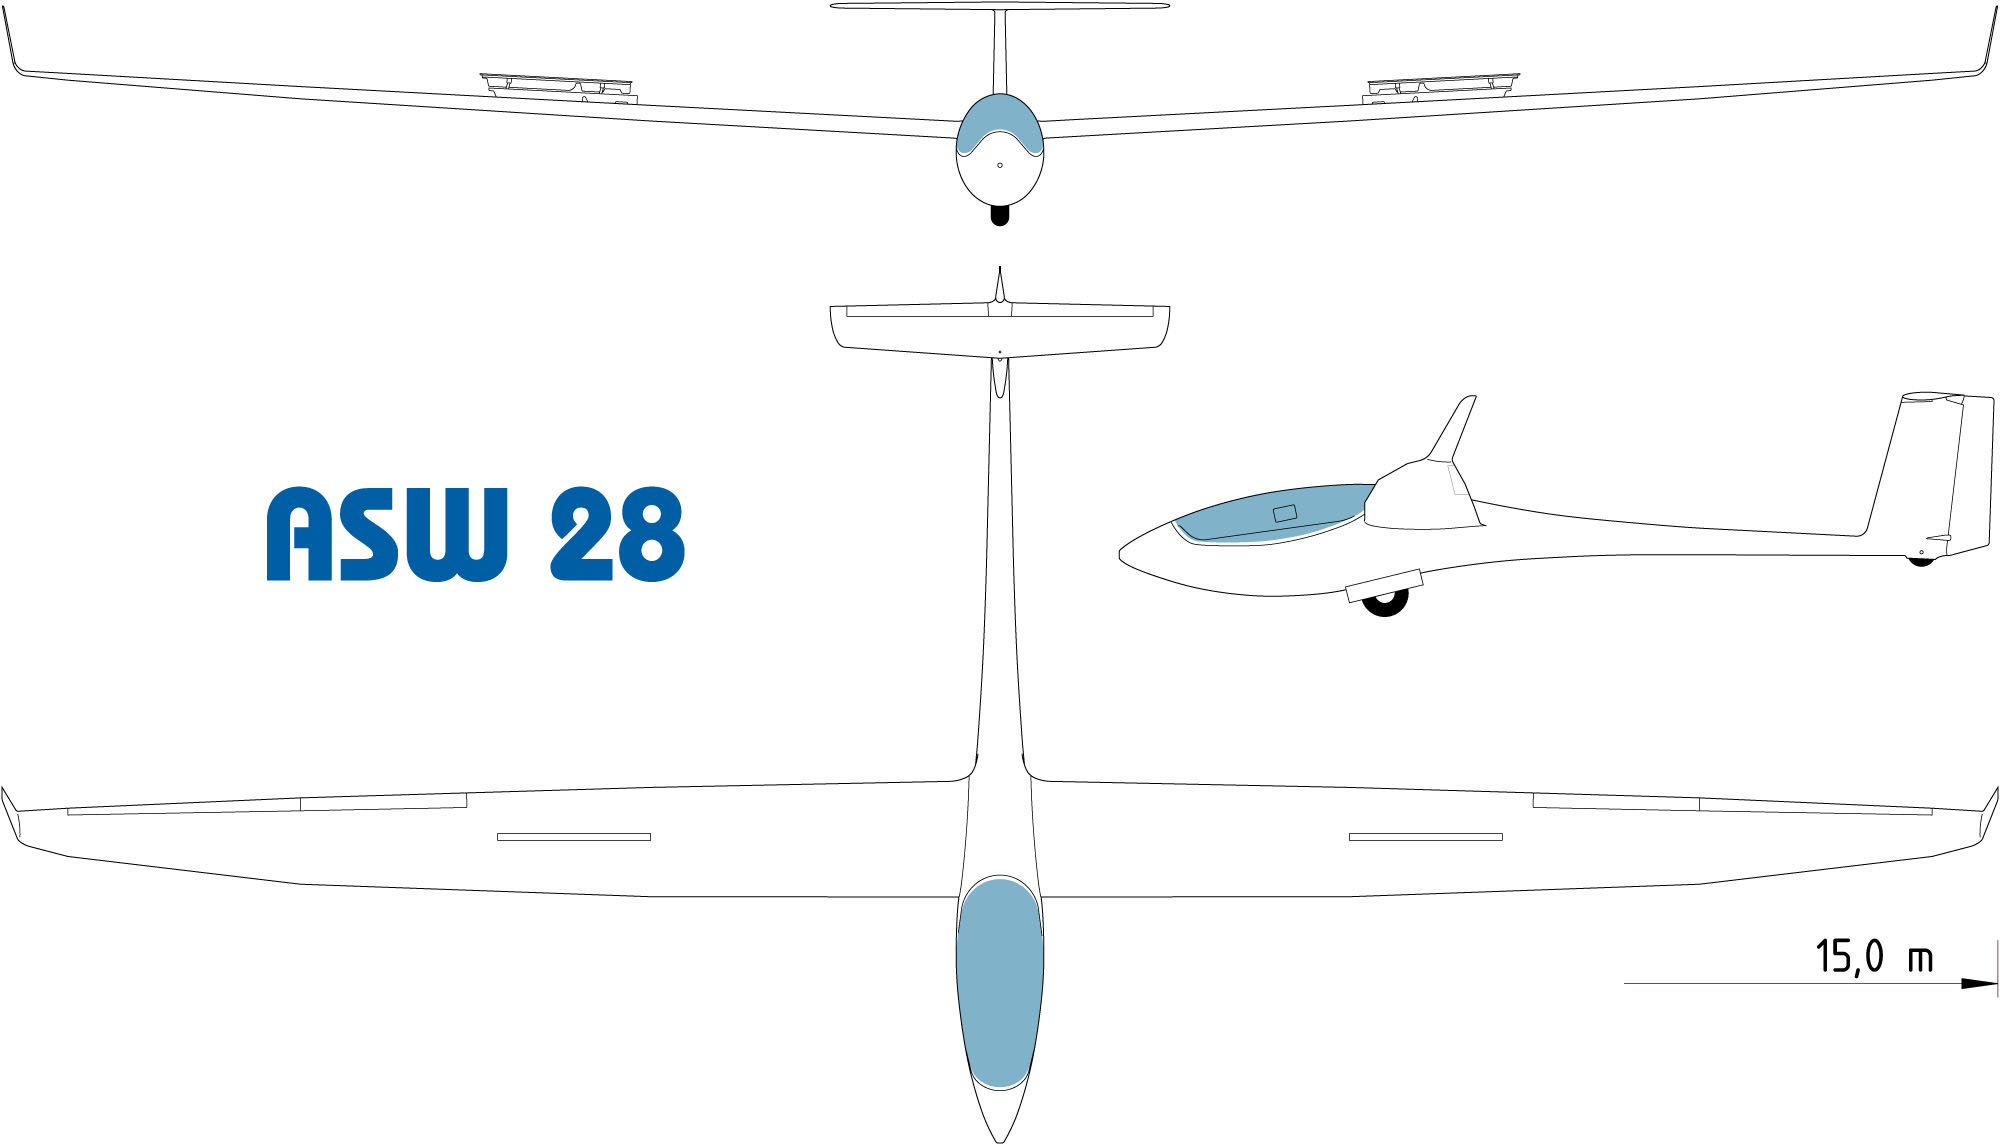
\includegraphics[width=5.5026in,height=3.34935in]{ASW 28 3side view.png}
\caption{Front, side and top view of ASW 28 glider \cite{asw28}}
\end{figure}

The analysis of the main Wing of the ASW 28 will include the following
steps:

\begin{enumerate}
\def\labelenumi{\arabic{enumi}.}
\item
  Model set up in Altair HyperMesh for modal analysis and flutter
  analysis
\item
  Creation of a Python script to read Flutter results from Optistruct
  solver
\item
  Definition of Optimization problem parameters using different
  optimization techniques and implementation using Python.
\end{enumerate}

\section{ASW 28 main Composite Wing Model}
\label{asw-28-main-composite-wing-model}

\subsection{Wing Geometry \&
Discretization}\label{wing-geometry-discretization}

The external geometry of the Wing was imported to HyperMesh from a CAD
file. The geometry was cleaned up so as to contain only the main wing of
the aircraft and because of some inaccuracies and the
non-metric length units used, a scale transformation had to be used.

\begin{figure}[H]
    \centering
    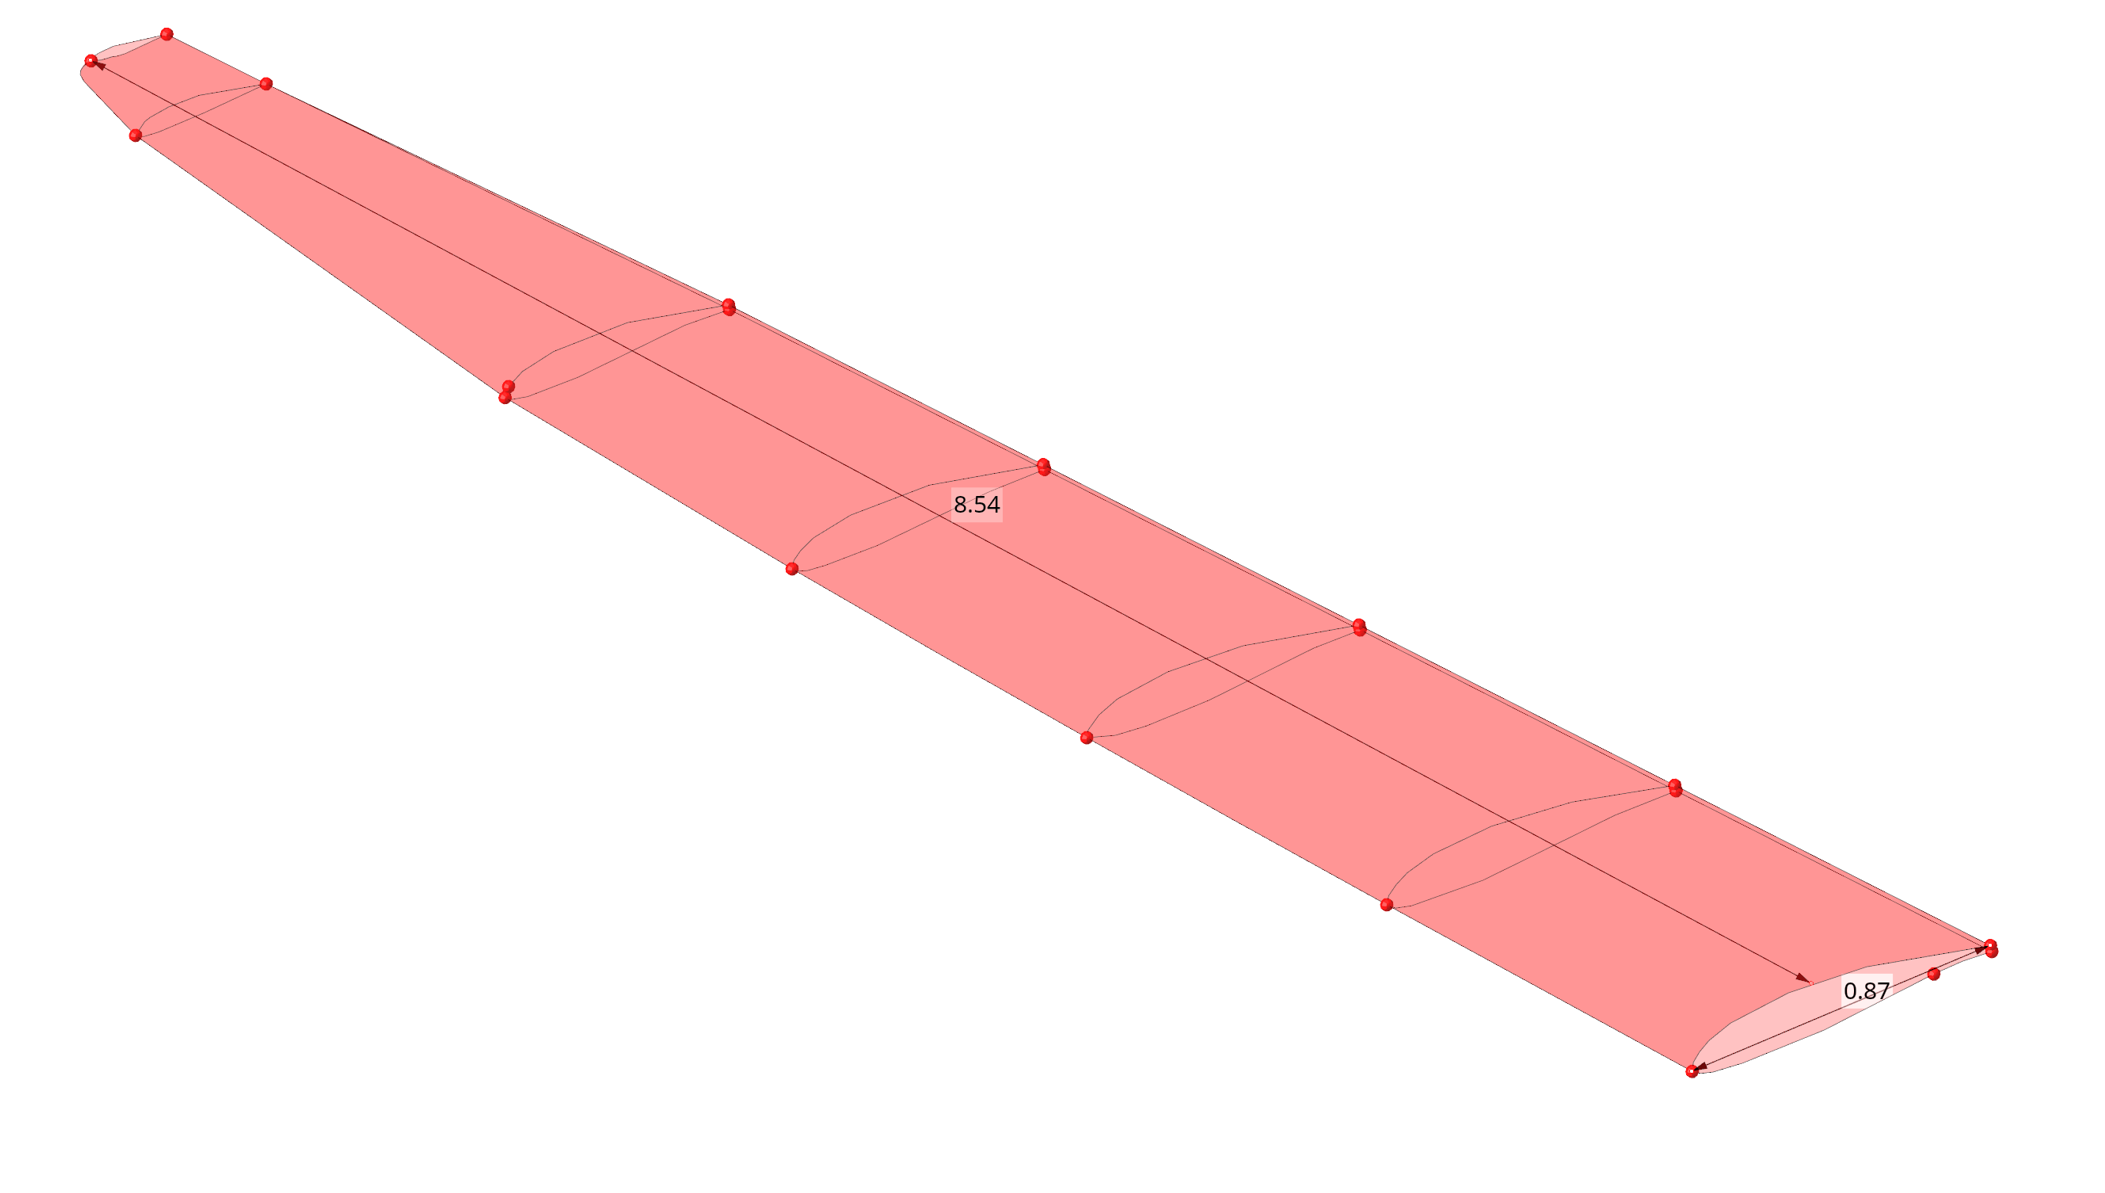
\includegraphics[width=\textwidth]{ASW 28 External Geometry.png}
    \caption{ASW 28 Wing external geometry (length in meters)}
\end{figure}

After the creation of the external geometry the internal structure of
the Wing had to be created from scratch. Since the detailed drawings of
the internal structure are not available, the internal structure
geometry was improvised based on some pictures of the disassembled wing.
The main features of most modern wings' internal geometry are the spars
and ribs. Spars are the main structural member of the wing which run
spanwise along the length of the wing and are responsible for carrying
aerodynamic loads to the main fuselage. Ribs are structural members of
the wing that run chordwise (perpendicular to the spars) and their
purpose is to support the wing's skin so that it maintains the proper
airfoil profile.

Modern glider wings usually have only one main spar and several ribs.
For this application a single main spar of rectangular cross section
which tapers towards the wing's tip and 6 ribs are used.

\begin{figure}[H]
    \centering
    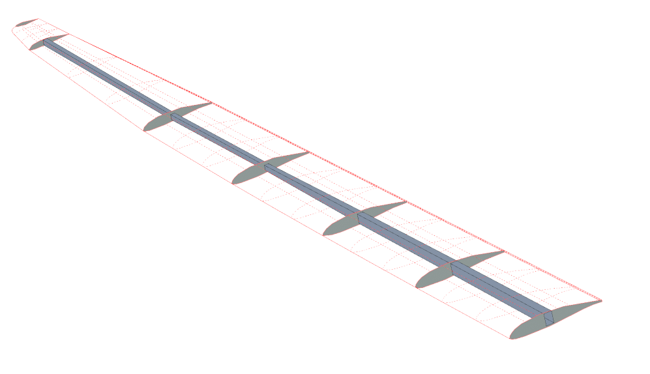
\includegraphics[width=\textwidth]{ASW 28 Internal Geometry.png}
    \caption{ASW 28 Wing Internal geometry}
\end{figure}


The discretization of the geometry was achieved using shell elements
arranged in a mesh which was created with the help of the ``Panel Mesh''
utility of HyperMesh for the skin of the wing since this function is
especially well suited for this type of panel-like geometry, and the
``General 2D Mesh'' utility for the internal geometry. The average
element size has a side length of \(0.02\ [m] \).

The discretization does not need to be very accurate since for the
flutter analysis we only need to capture enough detail to describe the
first few eigenmodes accurately and we do not care about the exact
stresses at specific points within the structure.

\begin{figure}[H]
\centering
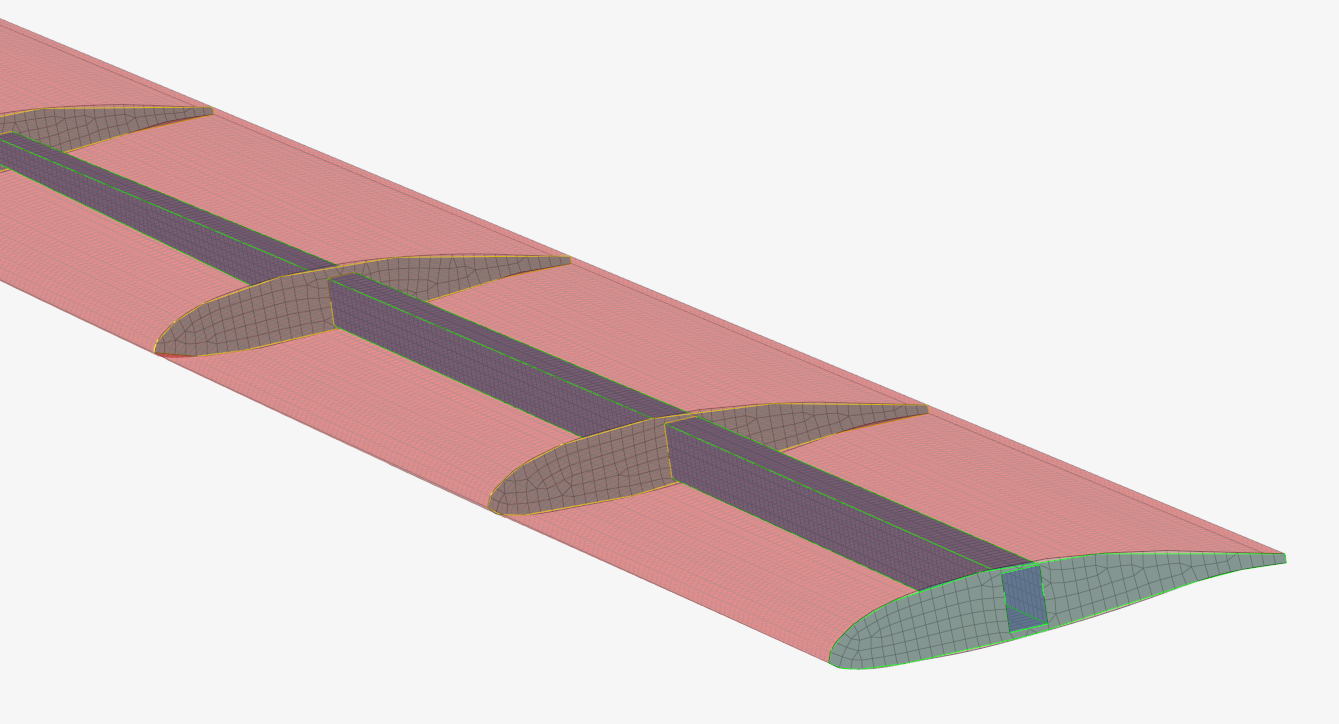
\includegraphics[width = \textwidth]{ASW 28 Wing Mesh.png}
\caption{ASW 28 Wing Internal mesh}
\end{figure}

\begin{figure}[H]
\centering
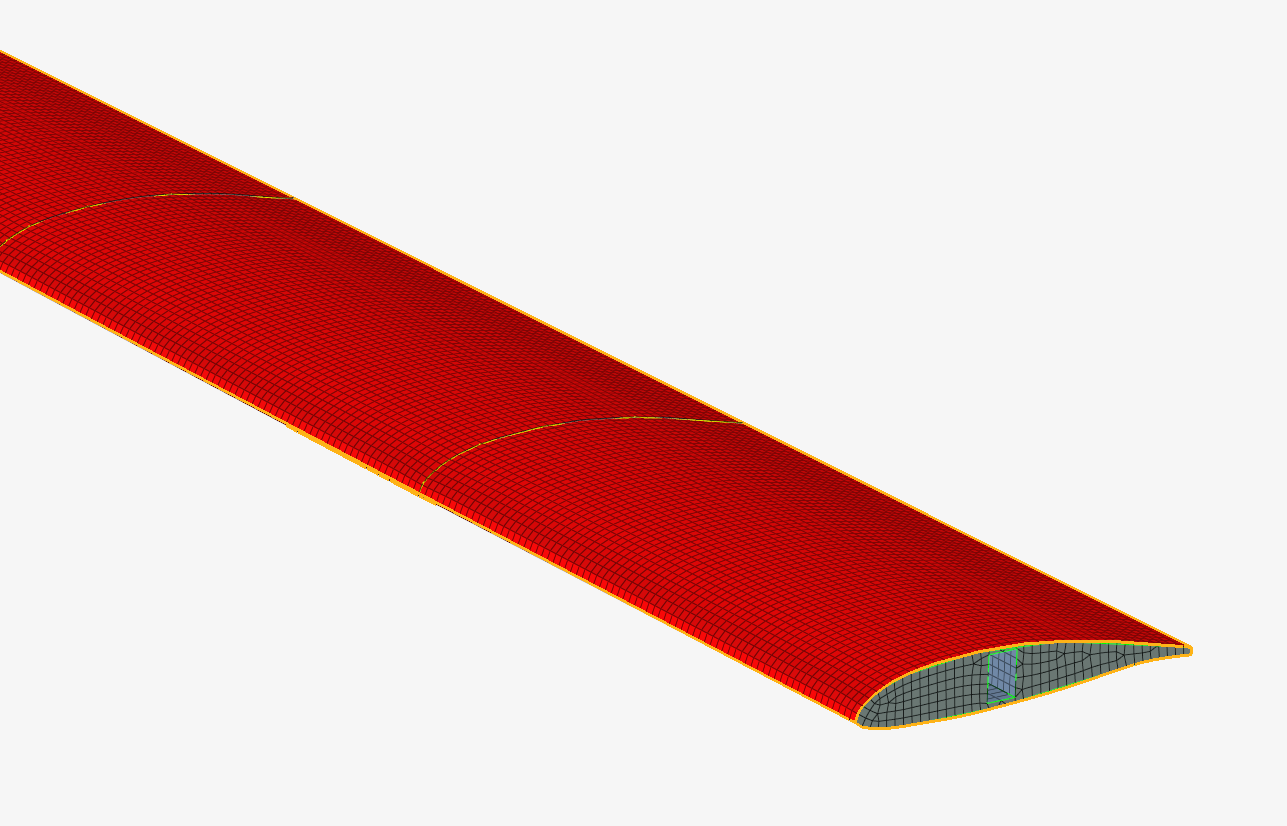
\includegraphics[width = \textwidth]{ASW 28 Wing Skin Mesh.png}
\caption{ASW 28 Wing skin mesh}
\end{figure}

\subsection{Material properties Definition}
\label{material-properties-definition.}

The material properties assigned to different components of the wing
structure are somewhat arbitrary as this information is not publicly
available. This should not pose any problems to the goal of this thesis
since during the optimization, material properties are subject to change
anyway.

A common composite material for the skin of high-performance gliders is
fiberglass or carbon fiber, because these materials offer high strength,
low weight and a smooth aerodynamic surface. For this application a
carbon fiber - Epoxy composite was chosen. For the Optistruct solver
this kind of composite material can be defined using the MAT8 material
card with the following properties \cite{matweb}:

\begin{itemize}
\item
  \(E_{1} = 125\ GPa\)
\item
  \(E_{2} = 8.41GPa\)
\item
  \(\nu_{12} = 0.35\)
\item
  \(G_{12} = 4.23\ GPa\)
\item
  \(\rho = 1517\ kg\text{/}m^{3}\)
\end{itemize}

This material is a laminated composite and although the material
properties have been sufficiently defined the laminate structure hasn't.
To define the laminate configuration a PCOMP property card is needed.
This card is essentially a list containing the properties of each
laminate layer. These properties are:

\begin{enumerate}
\def\labelenumi{\arabic{enumi}.}
\item
  The material of the laminate layer defined as a composite material
  card, in this case a MAT8 card
\item
  The thickness of each laminate layer defined as a float
\item
  The angle in degrees at which the primary axis (axis 1) of the
  laminate layer is oriented
\end{enumerate}

For this application a six-layer laminate composite will be created
using the carbon fiber epoxy orthotropic material with angles
alternating between +45 and -45 degrees and a thickness of \(0.5\ mm\)
for each layer.

For the internal structure of the wing an aviation grade aluminum is
used. More specifically aluminum 6061 is used, which has the following
properties:

\begin{itemize}
\item
  \(E = 69\ GPa\)
\item
  \(\nu = 0.33\)
\item
  \(\rho = 2700\ kg\text{/}m^{3}\)
\end{itemize}

This is an isotropic material and is defined within Optistruct with a
MAT1 card which essentially lists these material parameters in a
specific manner.

Similarly, the material definition alone is not enough as we are working
with shell elements, a property which defines the thickness of the
material need to be present. In Optistruct this property is defined
using a PSHELL property card which only needs to hold a material
reference and a thickness value. In this chase the thickness is uniform
everywhere and equal to \(t = 2mm\)

\subsection{Boundary Conditions} \label{boundary-conditions}

The boundary conditions defined for this problem are similar to that of
a fixed free cantilever beam. The nodes at the root of the wing are
fixed along every degree of freedom with an SPC (Single Point
Constraint) entry. These boundary conditions assume that the wing's root
is completely fixed on its support which works well for a detached wing
which is placed on a test bench but are only an approximation of the
real flight situation where the wing is fixed to the fuselage which is
not static during flight.

\begin{figure}[H]
\centering
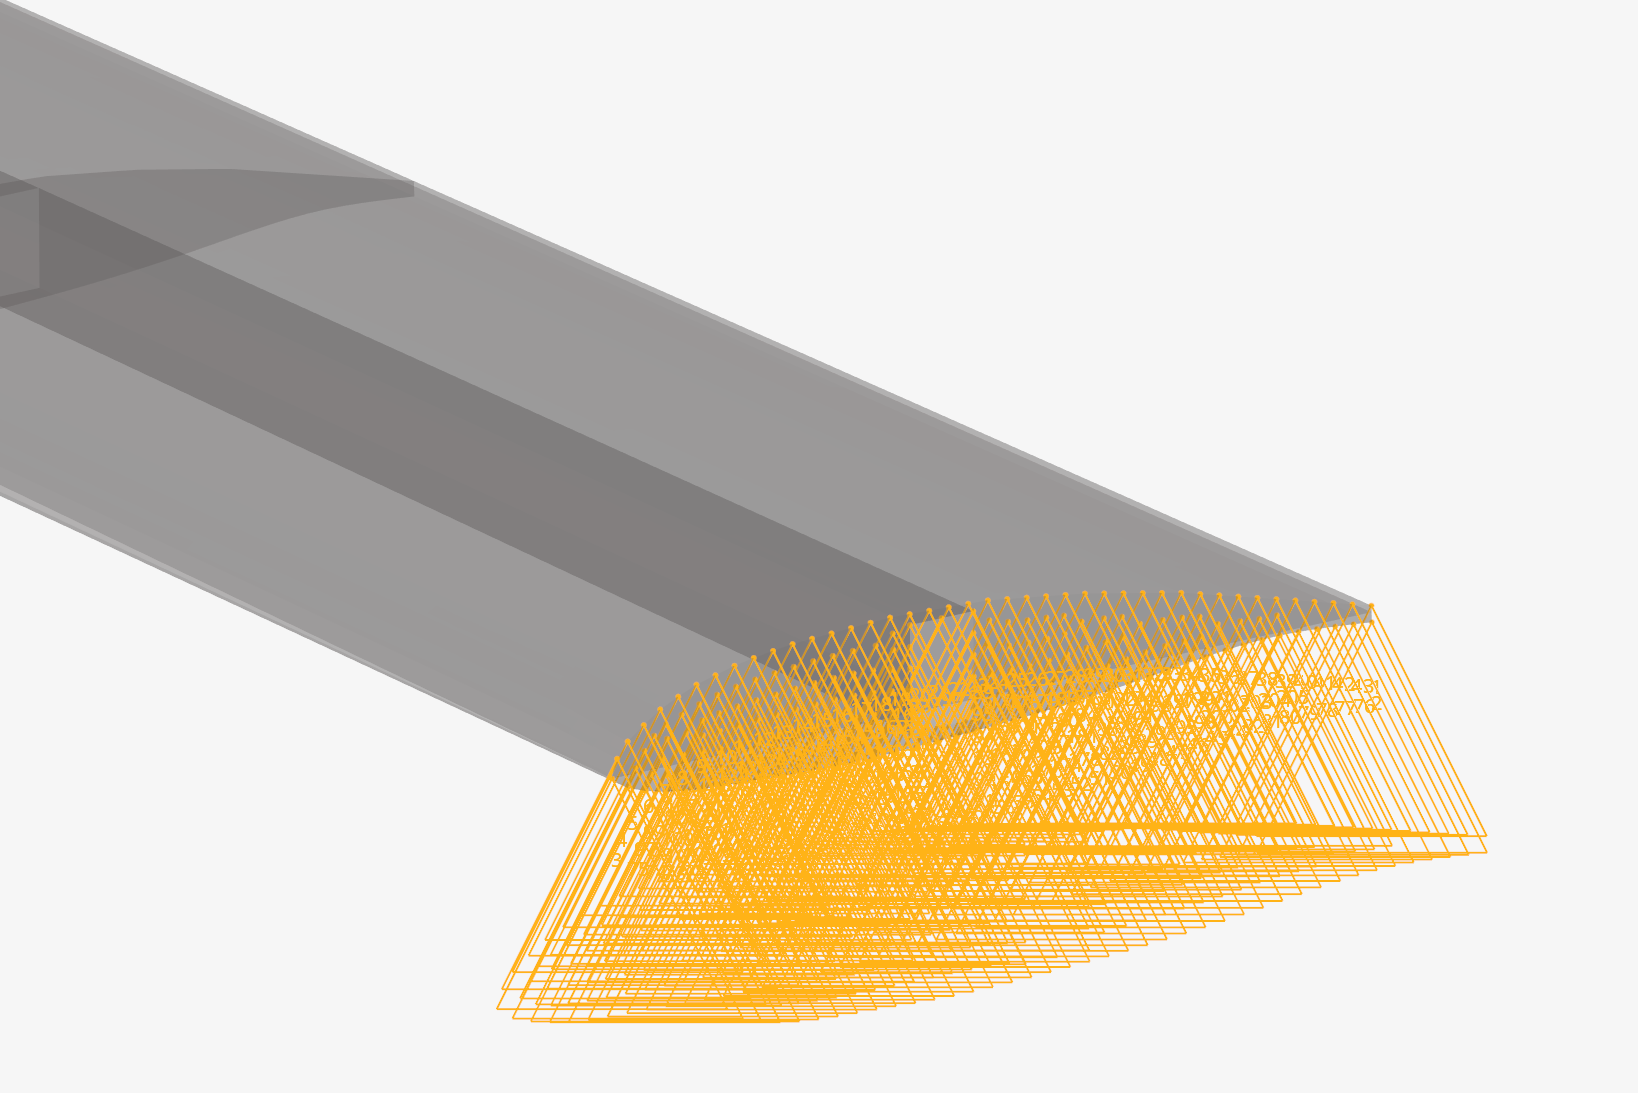
\includegraphics[width = \textwidth]{ASW 28 SPC.png}
\caption{ASW 28 Wing Boundary conditions}
\end{figure}

\subsection{Aerodynamic Grid}
\label{aerodynamic-grid}

To create the vortex-lattice the lifting surface of the wing needs to be
discretized. The way this is modeled in Optistruct is through the CAERO1
card which defines an ``aerodynamic macro element'' with a simple
two-dimensional quadrilateral geometry which is split into a predefined
number of boxes in the chordwise and spanwise directions. To define the
CAERO1 card one must first define the four corner points in a specified
order:

\begin{itemize}
\item
  The first point is on the leading edge and on the root of the wing
\item
  The second point has the same y coordinate as the first but lies on
  the trailing edge of the wing
\item
  The third point lies on the tip of the wing and at the trailing edge
\item
  The Fourth point has the same Y coordinate as the third but lies on
  the leading edge of the tip of the wing
\end{itemize}

\begin{figure}[H]
    \centering
    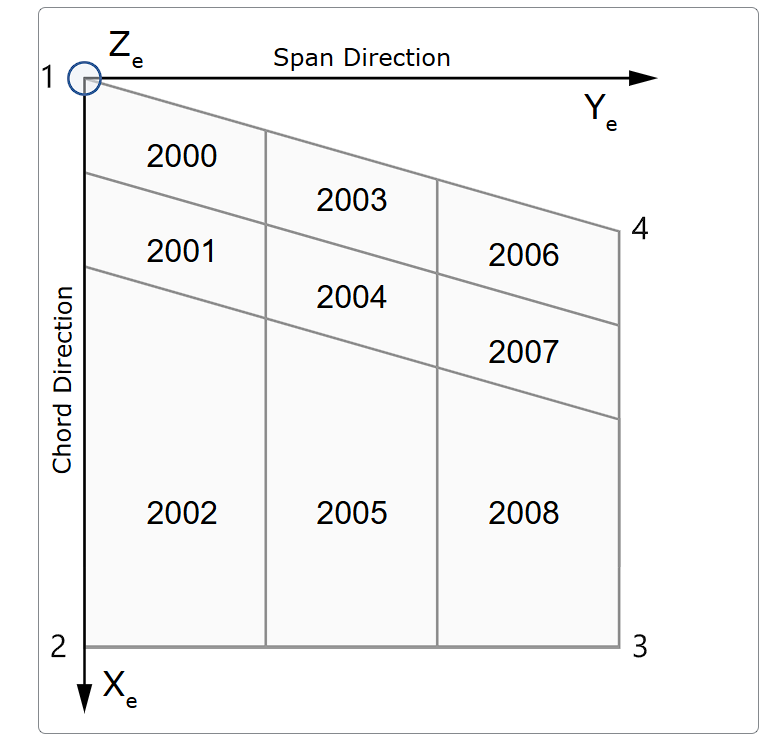
\includegraphics[width=0.6\textwidth]{CAERO1 Coordinate system.png}
    \caption{Coordinate System of CAERO1 Aerodynamic panel \cite{altair_flutter_tips}}
\end{figure}


This allows for the modelling of only simple trapezoidal geometries.
Since the projection of the ASW28 glider wing on the XY plane does not
fit well within a single trapezoidal shape two of these macro elements
were used to capture the variable taper ration of this wing. These
panels can be seen in the following image of the model.

\begin{figure}[H]
\centering
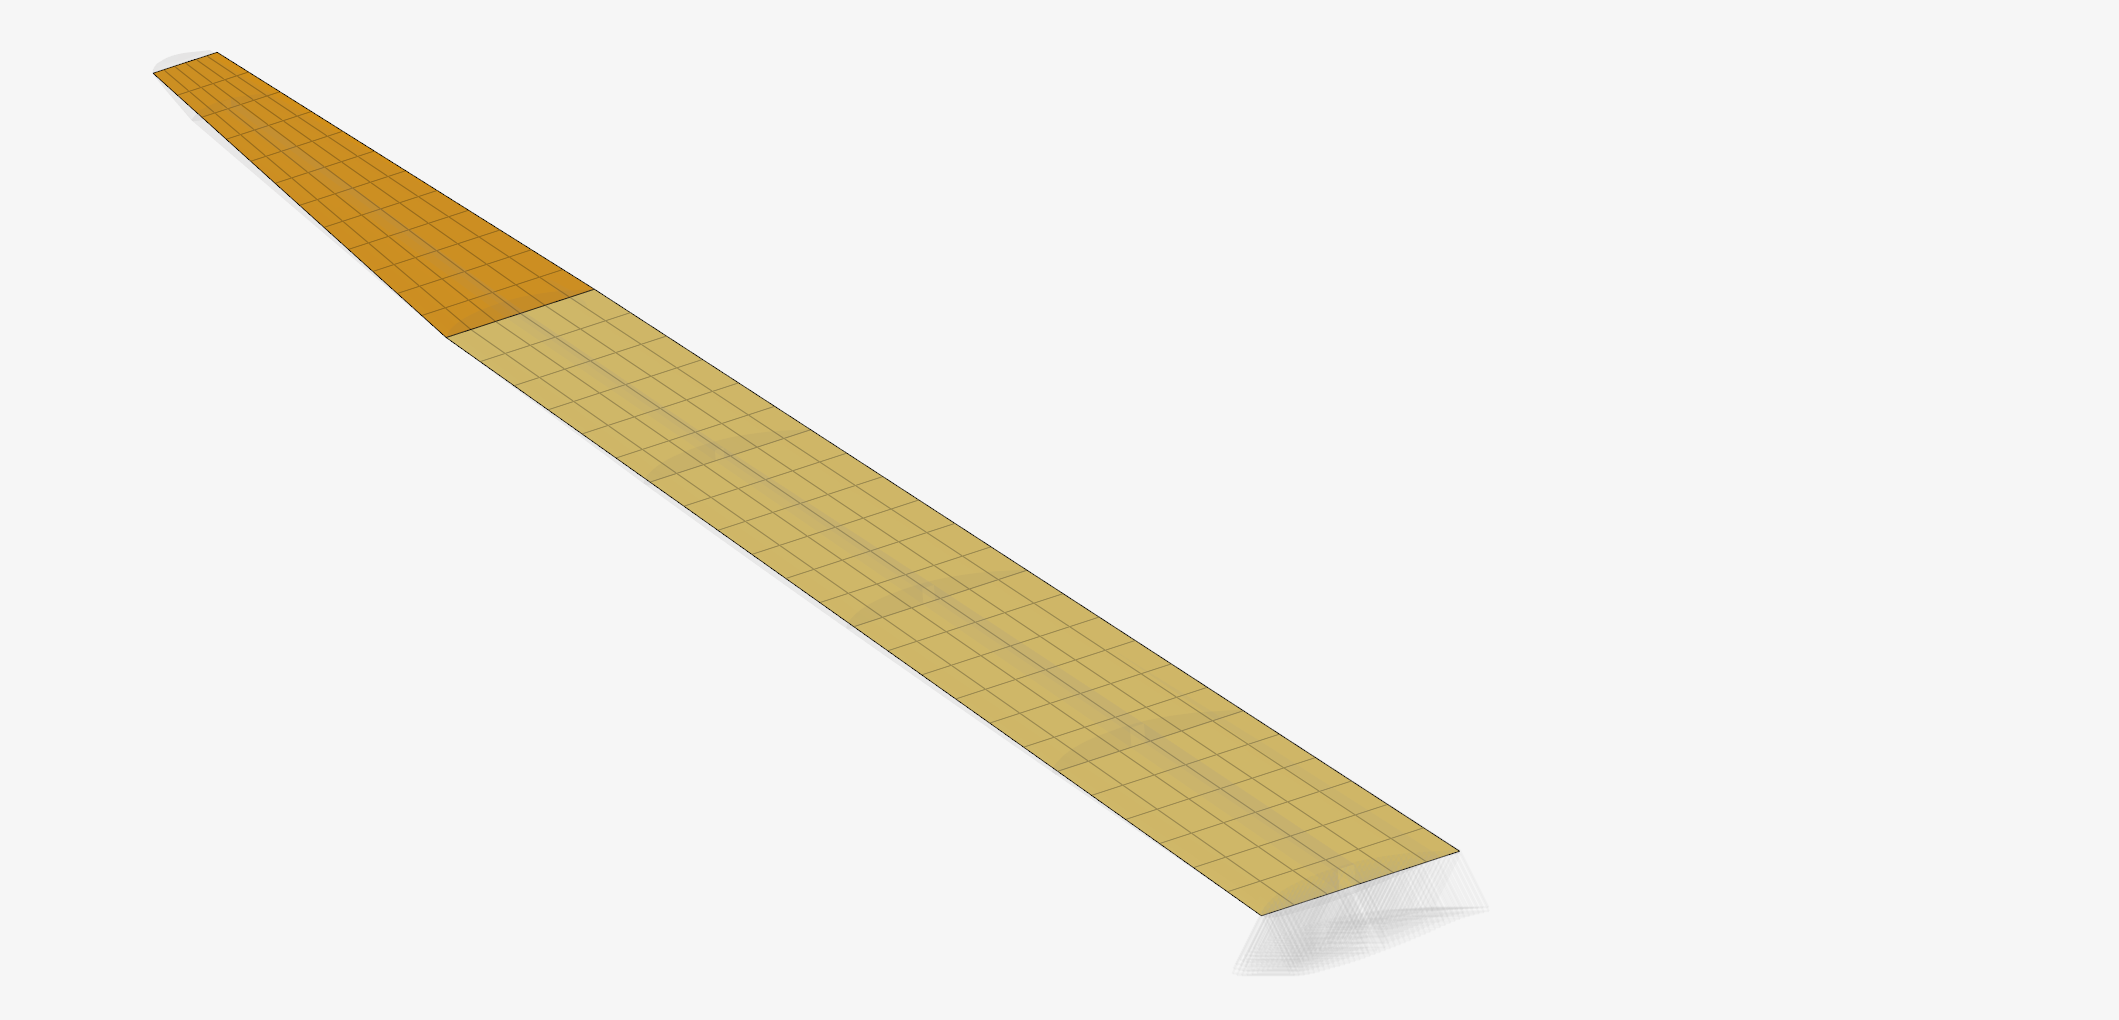
\includegraphics[width=4.65278in,height=3.01736in]{ASW 28 Aerodynamic grid.png}
\caption{CAERO1 macro elements of the ASW 28 Wing Model}
\end{figure}

The next step of defining the CAERO1 elements is defining the
discretization into aerodynamic boxes through two integer values NSAPN
and NCHORD which define the number of spanwise and chordwise boxes
respectively.

For the Inner CAERO1 macro element:

\[NSPAN = 24,\ \ NCHORD = 6\]

For the Outer CAERO1 macro element:

\[NSPAN = 12,\ \ NCHORD = 6\]

This discretization is chosen so that the aspect ratio of the boxes is
less than about three and the chordwise length of each box is less than
\(\Delta x < 0.08V_{\max}\ \text{/}f_{\max} \approx 0.65m\). These two
suggestions for the discretization of the aerodynamic panels are
specified in \cite{msc2021}

\subsection{The Spline}\label{the-spline}

In Flutter analysis the SPLINE entry is used to couple the structural
and aeroelastic domains. For this application a SPLINE1 entry is used
which defines a surface spline (linear splines are also available but do
not apply in this case.) To define the SPLINE1 the following entries are
needed:

\begin{itemize}
\item
  The CAERO Id which was defined in the previous step
\item
  The Id's of the first and last aerodynamic boxes to be included (All
  the aerodynamic panels are selected for this analysis)
\item
  A set of nodes from the structural grid
\end{itemize}

The selection of the structural nodes is important. Typically, not all
the nodes of the structure are selected. Only a subset of the nodes on
the bottom or upper surface of the wing are selected. These nodes need
to be under the area covered by the CAERO entry and the aerodynamic
boxes that were selected. Ideally each aerodynamic grid point has one
corresponding structural node directly above or below it, although this
is not feasible in most cases

\begin{figure}[H]
\centering
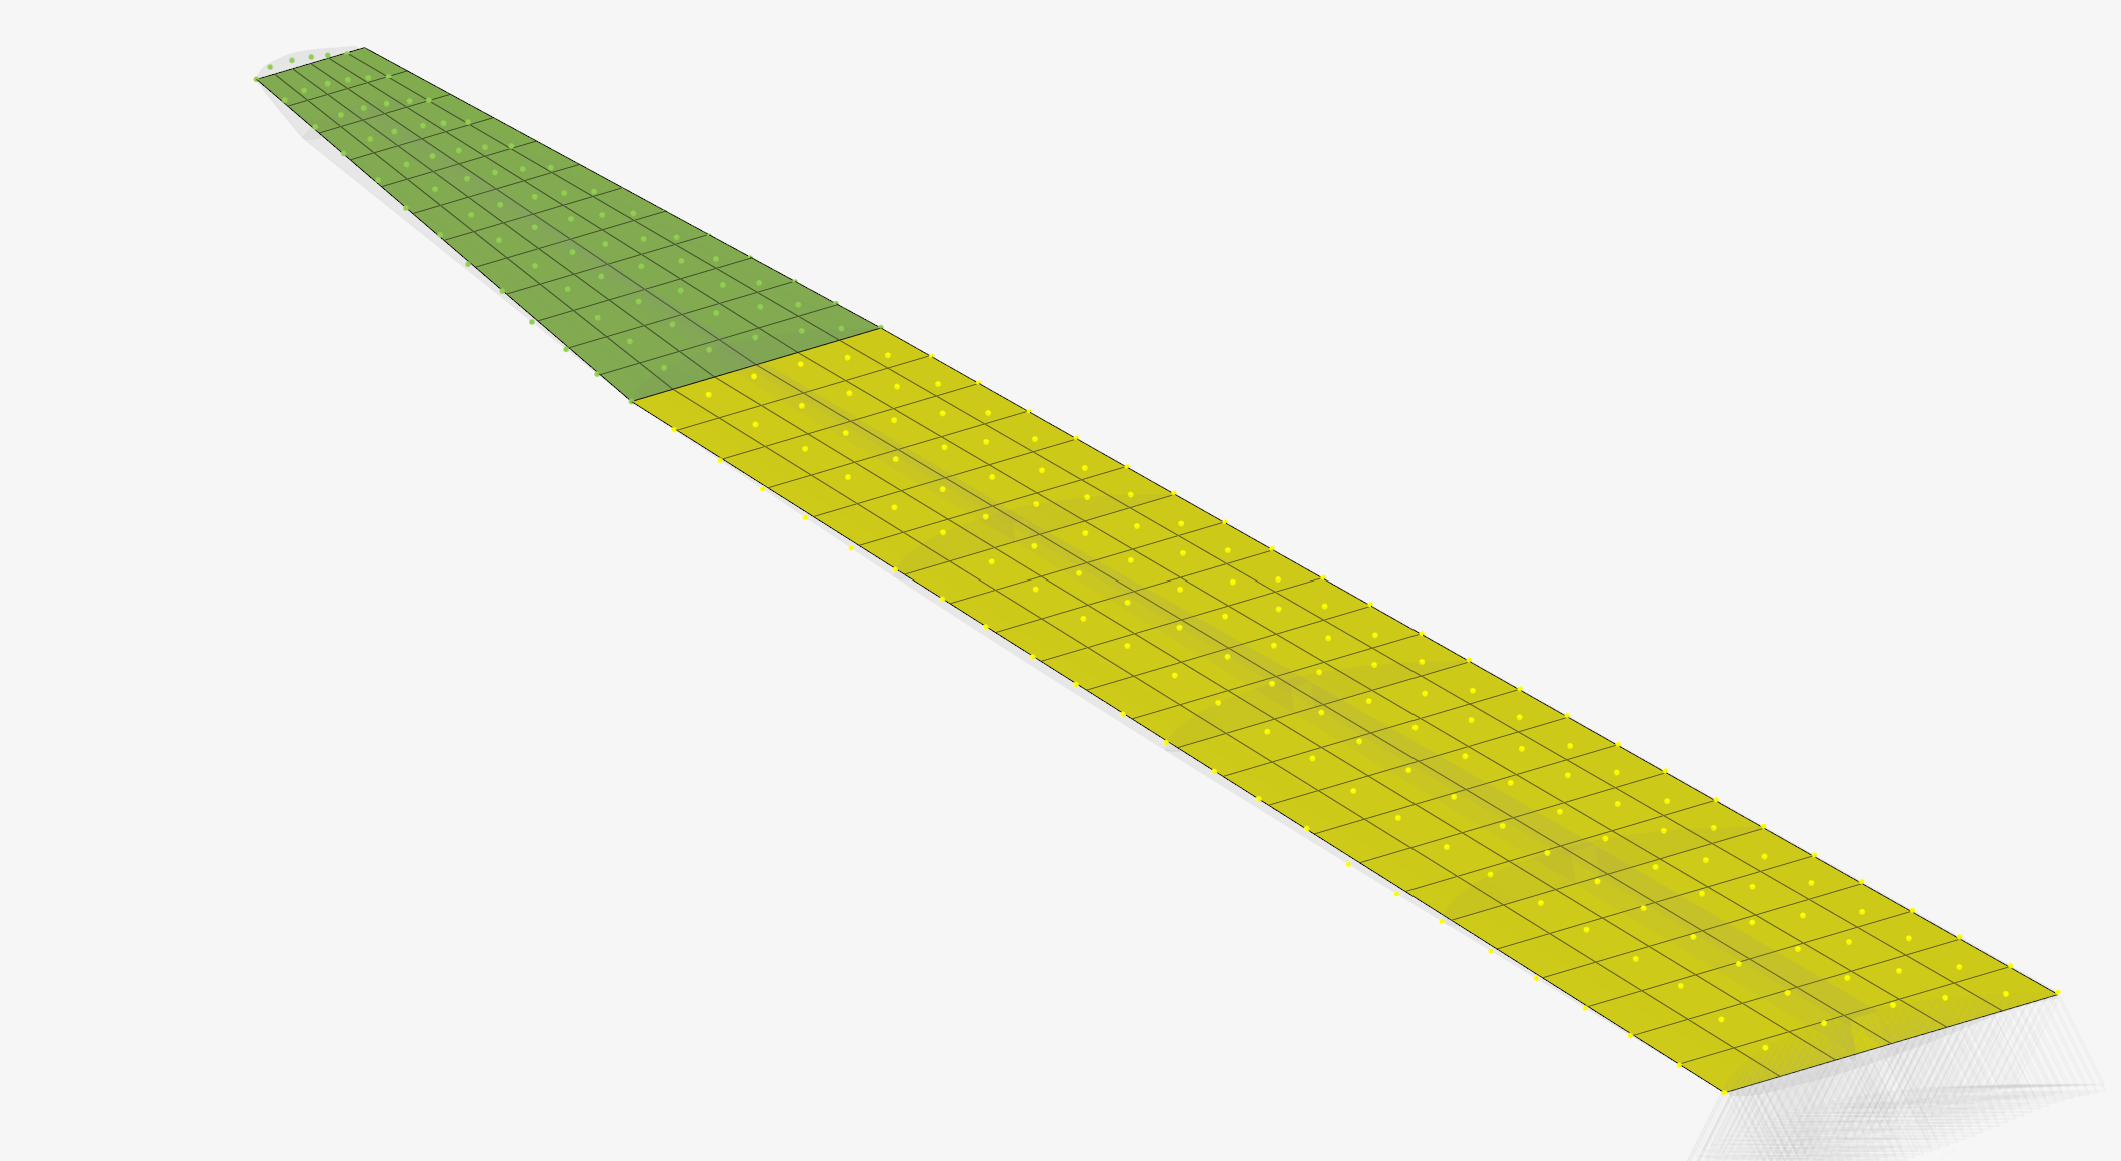
\includegraphics[width = \textwidth]{ASW 28 splines.png}
\caption{SPLINE1 entries of the ASW 28 Wing model}
\label{fig:SPLINE1}
\end{figure}

As can be seen in \autoref{fig:SPLINE1} two separate SPLINE1 entries were made in this model one for each CAERO entry defined previously. In this case nodes from the top surface of the wing are selected. The nodes are in series of along the span of the wing at various chord percentages, so as to closely match the aerodynamic grid points.

\subsection{Aeroelastic Problem Setup}
\label{aeroelastic-problem-setup}

To set up the Aeroelastic Flutter analysis several parameters need to be
defined.

\subsubsection{The AERO card:}

The AERO bulk data entry card defines basic parameters for dynamic
aeroelasticity regarding mainly the conditions of flight. The entries of
this card are summarized as follows:

\begin{itemize}
\item
  VELOCITY: has no effect for flutter analysis since the velocity
  varies during the analysis and defined elsewhere but cannot be left
  blank so unity is entered
\item
  REFC\textbf{:} Reference chord length used for the calculation of
  reduced frequency and lift and drag coefficients if requested
  \(REFC = 0.92m\)
\item
  RHOREF\textbf{:} Reference density \(RHOREF = 1.225\ kg\text{/}m^{3}\)
  which is the density of air at sea level
\item
  SYMXZ\textbf{:} which defines symmetry for the XZ plane and can have
  three values

  \begin{itemize}
  \item
    \textbf{-}1\textbf{:} for antisymmetry
  \item
    0: for no symmetry
  \item
    1: for symmetry
  \end{itemize}
\end{itemize}

\begin{quote}
for this application \(SYMZX\  = 1\)
\end{quote}

\begin{itemize}
\item
  \textbf{SYMXY:} defines symmetry for the XY plane in a similar way. In
  this analysis \(SYMXY = 0\)
\end{itemize}

\subsubsection{The MKAERO1 card:}

The MKAERO1 card is a bulk data entry card which is used to input a
table of Mach Numbers and Reduced Frequencies for which the aerodynamic
matrices are calculated.

The format of the MKAERO1 card has two column entries with a maximum of
eight elements each. One column is for the Mach number entry while the
other for the Reduced Frequencies. The aerodynamic matrices are computed
at every pair of values of reduced frequency and Mach number.

There are no concrete recommendations for the range of reduced
frequencies that must be covered by this entry, but since the
aerodynamic matrices are interpolated for the actual resultant reduced
frequency logic dictates that the range of reduced frequencies must be
at least greater than the resultant range of reduced frequencies. Of
course, this cannot be known a priori since the resultant reduced
frequencies are only made known after the analysis is run. For this
analysis quite a wide range of reduced frequencies was used after
consulting many examples of this type of analysis.

In case more than eight values are required for reduced frequency or
Mach number a second MKAERO1 entry can be made.

The values used are as follows:

\[\overrightarrow{M} = \begin{matrix}
0.0
\end{matrix},\ \ \overrightarrow{K} = \begin{bmatrix}
0.2 \\
0.4 \\
0.8 \\
1.6 \\
3.2 \\
6.4 \\
10 \\
14
\end{bmatrix}\]

As can be seen there is only one Mach number \(M = 0\) which means that
incompressible flow is assumed. The aerodynamic matrices are calculated
at every point \(\left( M_{i}, K_{j} \right)\)

\subsubsection{The FLFACT card:}

The FLFACT bulk data entry card is a card that specifies a series of
aerodynamic factors. These factors are used to define:

\begin{enumerate}
\def\labelenumi{\arabic{enumi}.}
\item
  Density ratios
\item
  Mach Numbers
\item
  Reduced Frequencies or Velocities (PK Method only).
\end{enumerate}

These factors can be defined using two different formats.

\begin{enumerate}
\def\labelenumi{\arabic{enumi}.}
\item
  In Format 1 a series of values is directly entered into the card
\item
  In Format 2 the so-called THRU format is used defining a series of
  values using:

  \begin{enumerate}
  \def\labelenumii{\alph{enumii}.}
  \item
    F1: The first factor
  \item
    FNF: the final factor
  \item
    NF: The Number of factors (integer)
  \item
    FMID: The intermediate aerodynamic factor
  \end{enumerate}
\end{enumerate}

The actual series of values produced when using the THRU format are
calculated using the following formula:

\begin{multline}
\frac{F1(FNF - FMID)(NF - i) + FNF(FMID - F1)(i - 1)}{(FNF - FMID)(NF - i) + (FMID - F1)(i - 1)}\\ ,where\ i = 1,2\ldots,NF
\end{multline}

Note that when \(FMID = \frac{F1 + FNF}{2}\) the factors are equally
distributed between F1 and FNF

For this Analysis three FLFACT Entries are needed:

\begin{itemize}
\item
  FLFACT 1: Is the density factor(s) and has a value of \(1\). This
  factor is multiplier of the Reference Density define in the AERO card
  and indicates that the analysis is to be performed at
  \(1 \times RHOREF\)
\item
  FLFACT 2: Is the Mach Number(s) and has a Value of \(0\). This factor
  is the Mach Number at which the analysis is to be performed.
\item
  FLFACT 3: Is the Velocity/ties at which the analysis is to be
  performed. This FLFACT is defined using the THRU Format with factors:

  \begin{itemize}
  \item
    \(F1\  = 20m/s\)
  \item
    \(FNF = 320m/s\)
  \item
    \(NF = 30\)
  \item
    \(FMID = 160\)
  \end{itemize}
\end{itemize}

The analysis is performed for every combination of combination of
density Mach number and velocity in the FLFACT entries

\subsubsection{The Flutter card:}

The flutter bulk data entry card specifies the method and parameters of
aeroelastic flutter analysis:

The most important fields of this card are

\begin{enumerate}
\def\labelenumi{\arabic{enumi}.}
\item
  METHOD the method can be one of K, PK, PKNL, KE for this analysis the
  PK method is used.
\item
  DENS: a reference to the FLFACT Bulk Data entry which specifies the
  density multipliers
\item
  MACH: a reference to the FLFACT Bulk Data entry which specifies the
  Mach number
\item
  VEL: a reference to the FLFACT Bulk Data entry which specifies the
  velocities
\item
  IMETH the interpolation method for the aerodynamic matrix which can be
  either L or S for linear or surface interpolation respectively. The
  default value of L is retained for this analysis
\end{enumerate}

\subsubsection{The EIGRL card:}

The EIGRL bulk data entry card defines the data required to perform real
eigenvalue analysis with the Lanczos method. The main fields of this
card are:

\begin{enumerate}
\def\labelenumi{\arabic{enumi}.}
\item
  V1, V2 Frequency range of analysis
\item
  ND Number of desired eigenfrequencies
\end{enumerate}

For this analysis, the Values \(V1 = 0.0\ Hz\) and \(ND = 8\) are used.
These values mean that the first eight eigenfrequencies starting from
zero Hertz will be calculated.

\subsubsection{Subcase Definition:}

For the subcase definition the ``Aerodynamic Flutter'' analysis type is
selected and then

\begin{itemize}
\item
  The FMETHOD field requires a reference to the Flutter card
\item
  The SPC Field requires a reference to the SPC load collector
\item
  The METHOD Field requires a reference to the EIGRL
\item
  The CMETHOD Field requires a reference to an EIGC card but can be left
  blank if no complex eigenvalues need to be computed (it is blank in
  this case since no structural damping is considered)
\item
  The SMETHOD Field requires a reference to a damping curve TDMP but can
  be left blank if structural damping is not considered. (it is blank in
  this case since no structural damping is considered)
\end{itemize}

The results of the aeroelastic flutter analysis are presented in \autoref{initial-flutter-analysis} 

\section{Optistruct -- Python Interface}\label{optistruct-python-interface}

\subsection{Results of Flutter Analysis \& Python }
\label{results-of-flutter-analysis-python}

The output of the analysis defined in the previous section is a .flt
text file in addition to the typical Optistruct .out output file. It has
a very specific format. It is organized in blocks of information each
corresponding to a different combination of Mach number, Density
(defined in the FLFACT entries) and Eigenmode number. The most important
aspects of the .flt file are outlined in \autoref{fig:Optistruct.fltfileexplanation} .

\begin{figure}[H]
    \centering
    \includesvg[width=\textwidth]{Flt file explanation.svg}
    \caption{Optistruct .flt file explanation}
    \label{fig:Optistruct.fltfileexplanation}
\end{figure}

The typical .out file, which is also output contains information about
whether the solver encountered any exceptions or warning and most
importantly information about the mass of the structure.

From the data contained in the .flt file two very useful plots can be
produced.

\begin{enumerate}
\def\labelenumi{\arabic{enumi}.}
\item
  The V-g plot plots the damping of each eigenmode (y-axis) against
  Velocity (x-axis)
\item
  The V-f plot plots the frequency of each eigenmode (y-axis) against
  Velocity (x-axis)
\end{enumerate}

\begin{figure}[H]
  \centering
  \begin{minipage}{0.495\textwidth}
      \centering
      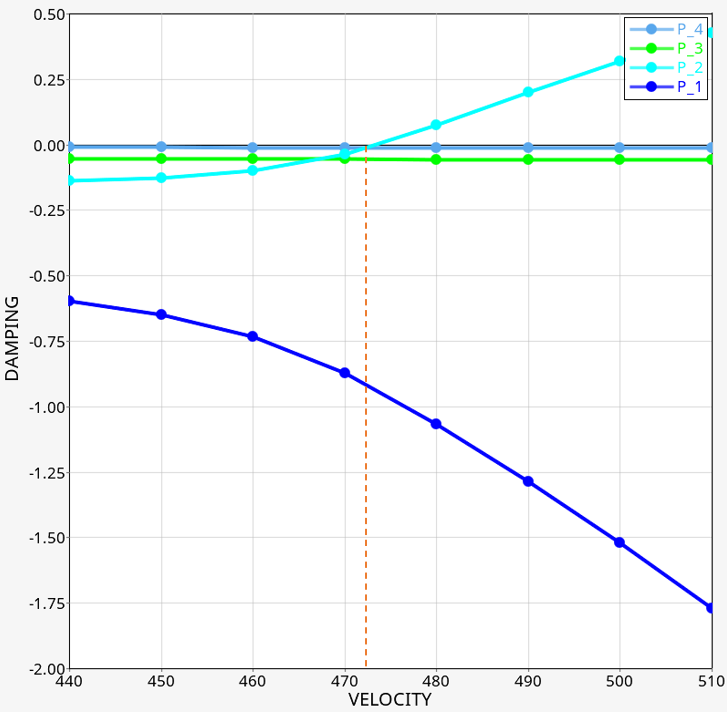
\includegraphics[width=\linewidth]{Example VG plot.png}
  \end{minipage}
  \hfill
  \begin{minipage}{0.495\textwidth}
      \centering
      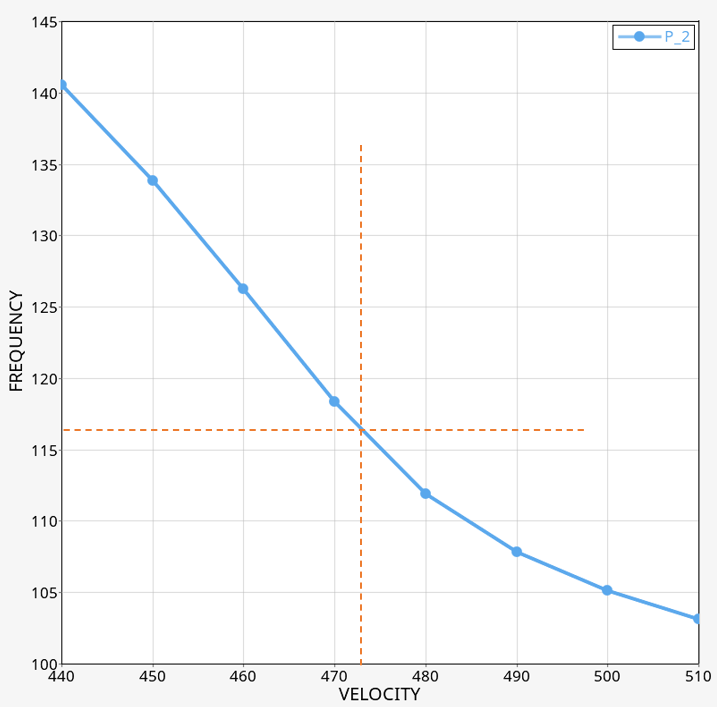
\includegraphics[width=\linewidth]{Example VF plot.png}

  \end{minipage}
  \caption{Example of V-g and V-f plot containing four eigenmodes \cite{altair_flutter_tips}}
\end{figure}


From these data one can determine the Flutter speed by examining the V-g
plot. More specifically a mode diverges when the damping of that
particular mode changes from negative to positive. Note that many modes
can diverge, but the flutter speed of the structure is determined by the
mode that diverges at the lowest speed.

The data blocks contained in the .flt file are read by a python script
and stored as pandas data frames. To determine the flutter velocity the
sign changes of each eigenmode are monitored until a negative to
positive change is detected. Then all the points where there is such a
sign change are stored and the flutter speed is determined by the
minimum speed at which such a sign change occurs.

A separate function is responsible for reading the .out file and
determining if the solver completed the analysis successfully as well as
recording the mass of the structure.

\subsection{Modifying Optistruct's input using
python}\label{modifying-optistructs-input-using-python}

In order to optimize the composite material of the structure one needs
to be able to modify the composite material's property programmatically
so that one can try many different variations and arrive at an optimum.
Optistruct makes this quite easy because it uses a text input file that
encodes all the information of the model. This file is called a .fem
file and can be output from HyperMesh as a comma separated text file. To
modify the composite material's property it is necessary to locate the
correct part of this file and decode it. According to Optistruct's
documentation the composite material's property is encoded in the
following way.

\begin{table}[h]
  \centering
  \resizebox{\linewidth}{!}{ % Fits table to page width
    \begin{tabular}{|c|c|c|c|c|c|c|c|c|c|}
      \hline
      1 & 2 & 3 & 4 & 5 & 6 & 7 & 8 & 9 & 10 \\ 
      \hline
      PCOMP & PID & Z0 & NSM & SB & FT & TREF & GE & LAM & + \\ 
      \hline
      & MID1 & T1 & THETA1 & SOUT1 & MID2 & T2 & THETA2 & SOUT2 & + \\ 
      \hline
      & MID3 & T3 & THETA3 & SOUT3 & Etc. & & & & \\ 
      \hline
    \end{tabular}
  }
  \caption{Table Fitted to Page Width}
\end{table}


Where:

\begin{itemize}
\item
  PCOMP: is the keyword indicating that a composite material property
  definition follows (string)
\item
  PID: is the ID of the property (integer)
\item
  NSM: is the non-structural mass per unit area (float)
\item
  SB: allowable inter lamina shear stress (default 0.0) (float)
\item
  FT: Failure Theory selection
\item
  TREF: Reference stress free temperature (float)
\item
  GE: Damping coefficient (float)
\item
  LAM: Laminate option different ways to define the laminate. In the
  default case all plies must be defined one by one
\item
  MIDi: The material ID of ply i (integer)
\item
  Ti: The thickness of ply i
\item
  THETAi: The angle of ply i
\item
  SOUTi: Stress, Strain output request default NO (bool)
\end{itemize}

The quantities to modify are mainly the Ti and THETAi entries to cover
the decision variables that will be needed.

\section{Optimization Problem}\label{optimization-problem}

In this chapter the implementation of the optimization algorithms
discussed in the theory \autoref{optimization-techniques} will be discussed.

\subsection{Applying Powell's method}\label{applying-powells-method}

This algorithm is implemented using SciPy's \cite{2020SciPy-NMeth} minimization
function by selecting the \emph{method = ``Powell''} optional argument.
In order to define the optimization problem some other important
parameters need to be defined.

\subsubsection{Decision Variables:}

The first step is the definition of the decision variables. These
variables consist of the thickness and angle of each layer in the
composite material. Since the composite laminate consists of six layers,
that would mean that 12 decision variables would have to be used.

Because of the computational time required though, some assumptions have
to be made in order to reduce the complexity of the optimization
problem. These assumptions are:

\begin{itemize}
\item
  The layers are antisymmetric.

This means that for every layer at height \(z_{k}\) with ply angle
\(\theta_{k}\) above the middle surface there exists an identical layer
with the opposite ply angle \(- \theta_{k}\) at height \(- z_{k}\) from
the middle surface


\begin{figure}[H]
    \centering
    \includesvg[width=0.7\textwidth]{Antisymmetric layers.svg}
    \caption{Antisymmetric layer configuration}
\end{figure}


This assumption reduces the number of decision variables for the ply
angles in half since from the original six independent variables only
three need to be defined for the six layered composite.
\([ \theta_{1},\ \ \theta_{2},\ \ \theta_{3}]\)

This assumption is reasonable since most composites are either symmetric
or anti symmetric in order to reduce the membrane - bending coupling
effects.


\item
  Each layer has the same thickness.

This assumption reduces the number of independent variables from six to
just one, since only one thickness \([t]\) needs to be
defined.

This assumption is also quite reasonable since during manufacturing of
composite parts every layer originates from the same spool of carbon
fiber which has an even thickness in its entirety.
\end{itemize}

These two assumptions lead to the final decision variables being:

\begin{equation}
\vec{\mathbf{x}}=[t,\theta_{1},\theta_{2},\theta_{3}]^{T}
\label{eq:descisionvars}
\end{equation}
\subsubsection{Objective function:}

Next the objective function is defined. Two different scenarios were
considered for the objective function.

\begin{itemize}
\item
  Scenario 1: The objective function considers the mass as well as the
  flutter velocity. The concept behind the formulation of this objective
  function is to be able to minimize the mass of the structure while
  maintaining a sufficient flutter speed. This would normally fall under
  the category of multi-objective optimization, but Powell's method
  doesn't allow for that, so a work around is used. The penalty method
  has to be employed, thus resulting in the following formulation.

\begin{equation}
    f_{obj}\left( \vec{\mathbf{x}} \right) =
    \begin{cases} 
        M, & V_{flutter} > V_{limit} \\
        M + P \cdot \left( V_{limit} - V_{flutter} \right), & V_{flutter} < V_{limit}
    \end{cases}
    \label{eq:objpowell1}
\end{equation}

\begin{quote}
Where:
\end{quote}

\begin{itemize}
\item
  \(M\): is the mass
\item
  \(P\): is a large constant called the penalty
\item
  \(V_{limit}\): is the limit below which the flutter speed of the wing
  is deemed unacceptably low
\item
  \(V_{flutter}\): is the resultant flutter speed from the Optistruct
  solver
\end{itemize}



This definition allows for the minimization of mass while keeping the flutter speed above a certain limit. If the flutter speed drops below the specified limit a penalty term proportional to the amount by which the constraint is violated is added to the objective function so that the optimization algorithm is forced to return to a region where the
constraint is not violated any more.


\item
  Scenario 2: The simpler scenario is an objective function where the
  input is the decision variable vector from equation \eqref{eq:descisionvars} but
  excluding the thickness \(t\), and the output is the negated flutter
  velocity calculated by the Optistruct solver.


\begin{equation}
f_{obj}\left( \vec{\mathbf{x}} \right) = - V_{flutter},\ \ with\ \vec{\mathbf{x}}\mathbf{=}\left\lbrack \theta_{1},\theta_{2},\theta_{3} \right\rbrack^{T}
\label{eq:objpowell2}
\end{equation}

The negative sign on the velocity is so that minimization occurs in the direction of increasing flutter velocity. Also notice that thickness has been removed from the optimization variables. Since mass is not considered in the objective function the optimizer could simply increase the thickness of the material and achieve a higher flutter speed this way. This behavior is of course undesirable and is the reason why thickness was removed from the optimization variables and now remains constant throughout the optimization process along with the mass of the wing.
\end{itemize}

\subsubsection{Search space boundaries}

To fully define the optimization problem, the search space needs to be fully defined. The boundary definition is quite simple in this case.

\begin{itemize}
\item
  For Scenario 1:\\
  The thickness has to be restrained in addition to the angles. The boundaries for the thickness are defined to be within a reasonable range
  of 0.1 to 1 mm per layer.

\begin{equation}
\theta_{1},\theta_{2},\theta_{3} \in [ - 90^{o}, + 90^{o} ]
\end{equation}


\item
  For Scenario 2:\\
  Only the angles need to be constrained between -90 and +90 degrees so
  the constraints are:



\begin{equation}
t \in [ 10^{- 4},\ 10^{- 3} ]\quad and \quad \theta_{1},\theta_{2},\theta_{3} \in [ - 90^{o}, + 90^{o} ]
\end{equation}
\end{itemize}



\subsubsection{Acceleration of the algorithm}
Because of the computationally intensive nature of the objective function a way to reduce computational time was applied. Instead of the algorithm being able to choose any arbitrary floating-point number within the specified range of each optimization variable a slight compromise was made. The values of each variable are internally rounded to a specified precision given by the user. Moreover, the results of each iteration are stored in a cache so that in case the algorithm finds itself trying to use the same input, the calculations are omitted and the cached results is used instead. The caching in combination with the rounding result in far fewer calls to the Optistruct solver than would be otherwise required. In this application the angles are rounded to the nearest integer while the thickness is rounded to the nearest tenth of a
millimetre.

To illustrate this concept more clearly an example will be made:\\

Let's assume that the initial vector is
\({\vec{x}}_{0} = \lbrack 0.0005,\ \ 45,\  - 45,\ 45\rbrack^{T}\)

\begin{enumerate}
\def\labelenumi{\arabic{enumi}.}
\item
  For the first iteration let's assume that the algorithm tries


\[{\vec{x}}_{1} = \lbrack 0.00043,\  - 20.3,\  - 69.6\ ,\ 42.14\rbrack^{T}\]

this will internally get rounded to

\[{\vec{x}}_{1} = \lbrack 0.0004,\ \ 20,\  - 70,\ 42\rbrack^{T}\]

and the result will be cached

\item
  If in the second iteration the algorithm tries
\end{enumerate}

\[{\vec{x}}_{2} = \lbrack 0.00041,\  - 20.4,\  - 69.8\ ,\ 42.47\rbrack^{T}\]

it will still get rounded to

\[{\vec{x}}_{2} = \lbrack 0.0004,\ \ 20,\  - 70,\ 42\rbrack^{T}\]

and the same cached result will be used

The results of Powell's method are presented in \autoref{powells-optimization-method}


\subsubsection{Applying the Genetic Algorithm}
\label{applying-the-genetic-algorithm}

For the application of the genetic algorithm the PyGAD \cite{gad2023pygad} library
is used. In order to define the optimization problem for the genetic
algorithm many parameters need to be defined. Unfortunately, there is no
way of finding the optimal settings for every variable in every specific
problem. Therefore, the parameters were chosen after some
experimentation using a smaller number of generations which can be run
faster. The parameters that are selected are most probably not the most
optimal but work well enough.

\begin{enumerate}
\def\labelenumi{\arabic{enumi}.}
\item
  First and foremost, the \textbf{genes} and the \textbf{gene}
  \textbf{space} must be decided.

The genes are analogous to the optimization variables of classical
optimization algorithms and are chosen to be the three angles and the
thickness of the layers so four genes in total.

A range of possible values needs to be defined for every gene. The range
for every angle gene is:

\[\vartheta_{RANGE} = \lbrack - 90,\  + 90,\ step = 1\rbrack\]

and for the thickness:

\[t_{RANGE} = \lbrack 0.0001,\ 0.001,\ step = 0.0001\rbrack\]

these ranges define the gene space.

\item
  The so-called fitness function needs to be defined. The fitness
  function is analogous to the objective function of classical
  optimization algorithms. Because of the advanced abilities of this
  algorithm a multi-objective optimization is carried out where the two
  goals are:

  \begin{itemize}
  \item
    The minimization of the mass of the ASW 28 Wing structure
  \item
    The maximization of the Flutter Velocity.To achieve those goals a
    function is created with the following format
  \end{itemize}

\begin{equation}
f_{fitness}\left( \begin{bmatrix}
t \\
\vartheta_{1} \\
\vartheta_{2} \\
\vartheta_{3}
\end{bmatrix} \right)\  = \begin{bmatrix}
 - Mass \\
V_{flutter}
\end{bmatrix}
\end{equation}


The negative sign for the mass is because this algorithm works on
maximizing the fitness function.
\end{enumerate}


After those basic and mandatory inputs are defined, several other
parameters which control the way the algorithm runs are defined.


\begin{itemize}
\item
  \emph{Num\_generations = 1000, controls} the number of generations in
  the span of which evolution will take place. This parameter is chosen
  so that a reasonable computational time is maintained
\item
  \emph{sol\_per\_pop = 10,} the number of solutions that will be
  produced (number of chromosomes) after each generation
\item
  \emph{parent\_selection\_type = steady state selection}
\item
  \emph{keep\_elitisism = 4} which means that the four best solution of
  each generation are carried over to the next
\item
  \emph{crossover\_type = ``single point''}
\item
  \emph{crossover\_probability = 0.7} The probability of selecting a
  parent for applying the crossover operation. For each parent, a random
  value between 0.0 and 1.0 is generated. If this random value is less
  than or equal to the value assigned to the crossover\_probability
  parameter, then the parent is selected.
\item
  \emph{mutation\_type = ``random''}
\item
  \emph{mutation\_probability = 0.1} The probability of selecting a gene
  for applying the mutation operation. For each gene in a solution, a
  random value between 0.0 and 1.0 is generated. If this random value is
  less than or equal to the value assigned to the mutation\_probability
  parameter, then the gene is selected
\item
  \emph{mutation\_by\_replacement = True,} means replace the gene by the
  randomly generated value instead of adding the random value to it.
\end{itemize}

The results of the Genetic Algorithm are presented in \autoref{genetic-algorithm-optimization}


\subsection{Flutter Speed Prediction using Neural networks}
\label{flutter-speed-prediction-using-neural-networks}

The purpose of this section is to develop a surrogate model using Neural
Networks in order to potentially accelerate the process of optimization.
Surrogate models are often used in engineering when the outcome of
interest is not easily measured or when the computational effort
required for proper simulation is too great. The development of the
Neural Network models is done in python using the Keras library from
Tensorflow.

The development of neural networks is a multistep process.

\begin{enumerate}
\def\labelenumi{\arabic{enumi}.}
\item
  The training data for the models have to be collected and organized in
  a convenient way
\item
  The structure of the model and its parameters have to be defined
\item
  The model has to be trained on the training data
\item
  Lastly the performance of the network has to be evaluated
\end{enumerate}


\subsubsection{Training Data}

To acquire the training data the solver is run repeatedly for random
material parameters within specified ranges. The parameters that vary
are the same as those used for the optimization.

More specifically those parameters are:

The angle of the major axis of each layer assuming an antisymmetric
construction

\begin{equation}
\theta_{i} \quad \in [ - 90^{o}, + 90^{o}], \quad for\ i = 1,2,3
\end{equation}


The thickness of each layer assuming all the layers have equal thickness

\begin{equation}
t \quad \in [ 0.1, 0.9]\ mm
\end{equation}

3000 random datapoints were collected and organized in a data frame
where every row represents a data point and contains information about
the input variables used and the predicted flutter speed from Optistruct
which is the target variable of the Neural Network. The mass of the wing
was also recorded but this is not a target variable for the neural
networks that are about to be developed because the mass is directly
proportional to the thickness of the layers. \(Mass \propto t\). The
computational time required to gather all the data is approximately 23
hours.


\subsubsection{Model Structure \& parameters}

The structure of the layers is a very important aspect of neural
networks. There is no way to know a priori the optimal structure of the
neural network so that a good prediction is made, and a reasonable
training time is achieved. For this reason, many different models will
be created, and their performance will be evaluated in order to find the
best one.

The first layer of every Neural Network is a normalization layer. This
is an important step that ensures a consistent scale between the
different data types of the input. In turn this ensures that no feature
dominates the learning process. Furthermore, normalization can improve
convergence by keeping the weights and activations within a reasonable
range. Lastly normalization can help by reducing the overfitting and
making a model more robust.

For this example, the two different kinds of inputs (the angles and the
thickness) have very different ranges since the angles vary between -90
and +90 while the thicknesses are four orders of magnitude smaller
varying between 0.0001 and 0.001 meters.

The normalization layer in Keras shifts and scales the input data into a
distribution centered around 0 and with a standard deviation of 1 by
subtracting the mean of the training data and the dividing by the square
root of the variance in the data.

\begin{equation}
f_{norm}(x) = \frac{x - mean\left( \overrightarrow{x} \right)}{\sqrt{var\left( \overrightarrow{x} \right)}}
\end{equation}

The mean and variation of the data is calculated based on the training
data. If the training data is not representative of the actual data on
which the network will be called to make predictions on, the
normalization might fail producing a non-centered distribution with a
variation much different than 1.

After the normalization layer the hidden layers follow. These layers
differ in number from model to model. In this work Neural Networks with
1, 2, 4, and 6 hidden layers will be tested. Each layer has 64 Neurons
and uses the RELU activation function.

Finally the output layer is added which uses a linear activation function
as this is a regression problem and only has 1 Neuron because the only
prediction that these neural networks make is the flutter speed of the
ASW 28 Wing model.

\begin{figure}[H]
  \centering
  \begin{minipage}{0.4\textwidth}
      \centering
      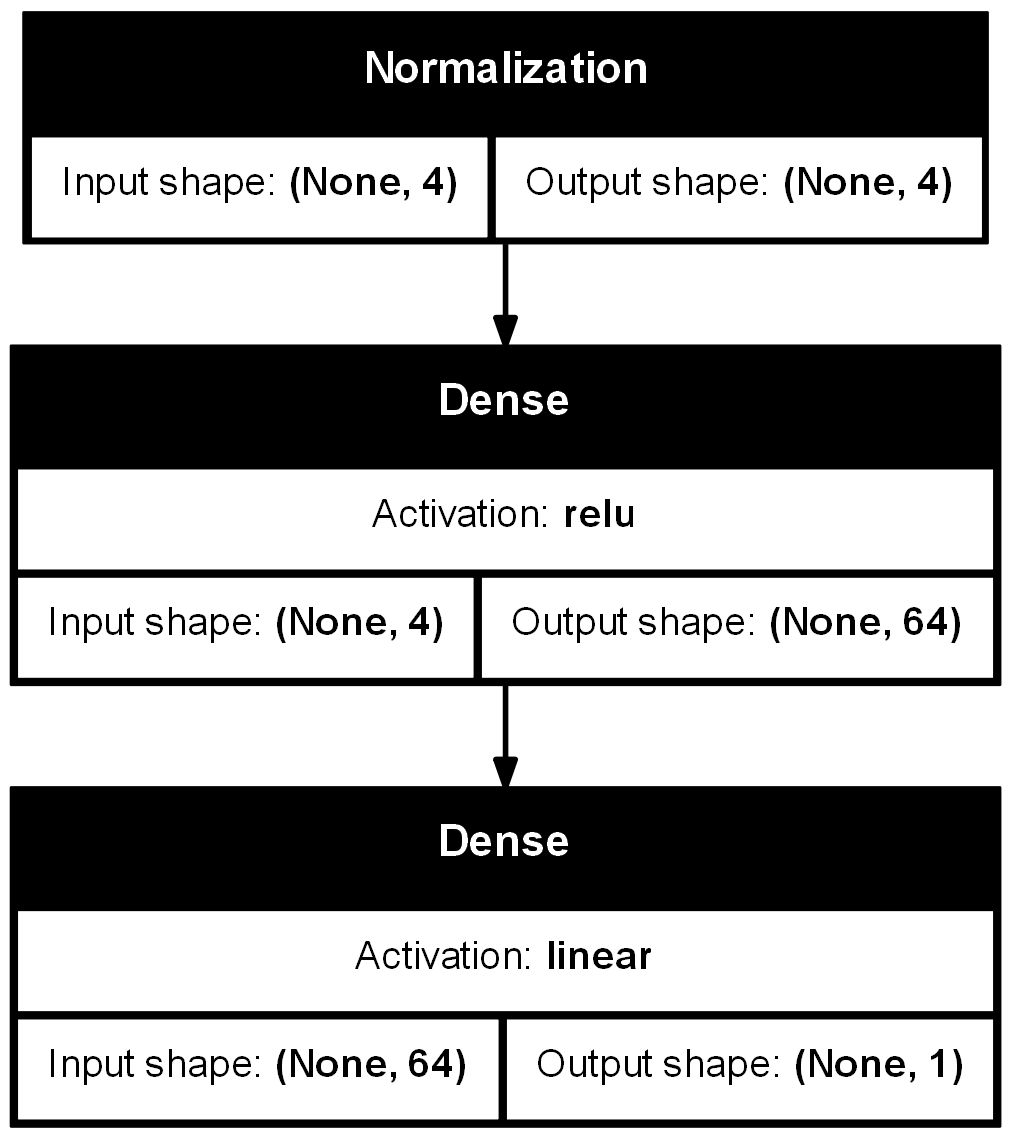
\includegraphics[width=\linewidth]{images/Results/Neural Net/1HL/structure.png}
      \caption{Neural Network Structure with $1$ Hidden layer}
  \end{minipage}
  \hfill
  \begin{minipage}{0.4\textwidth}
      \centering
      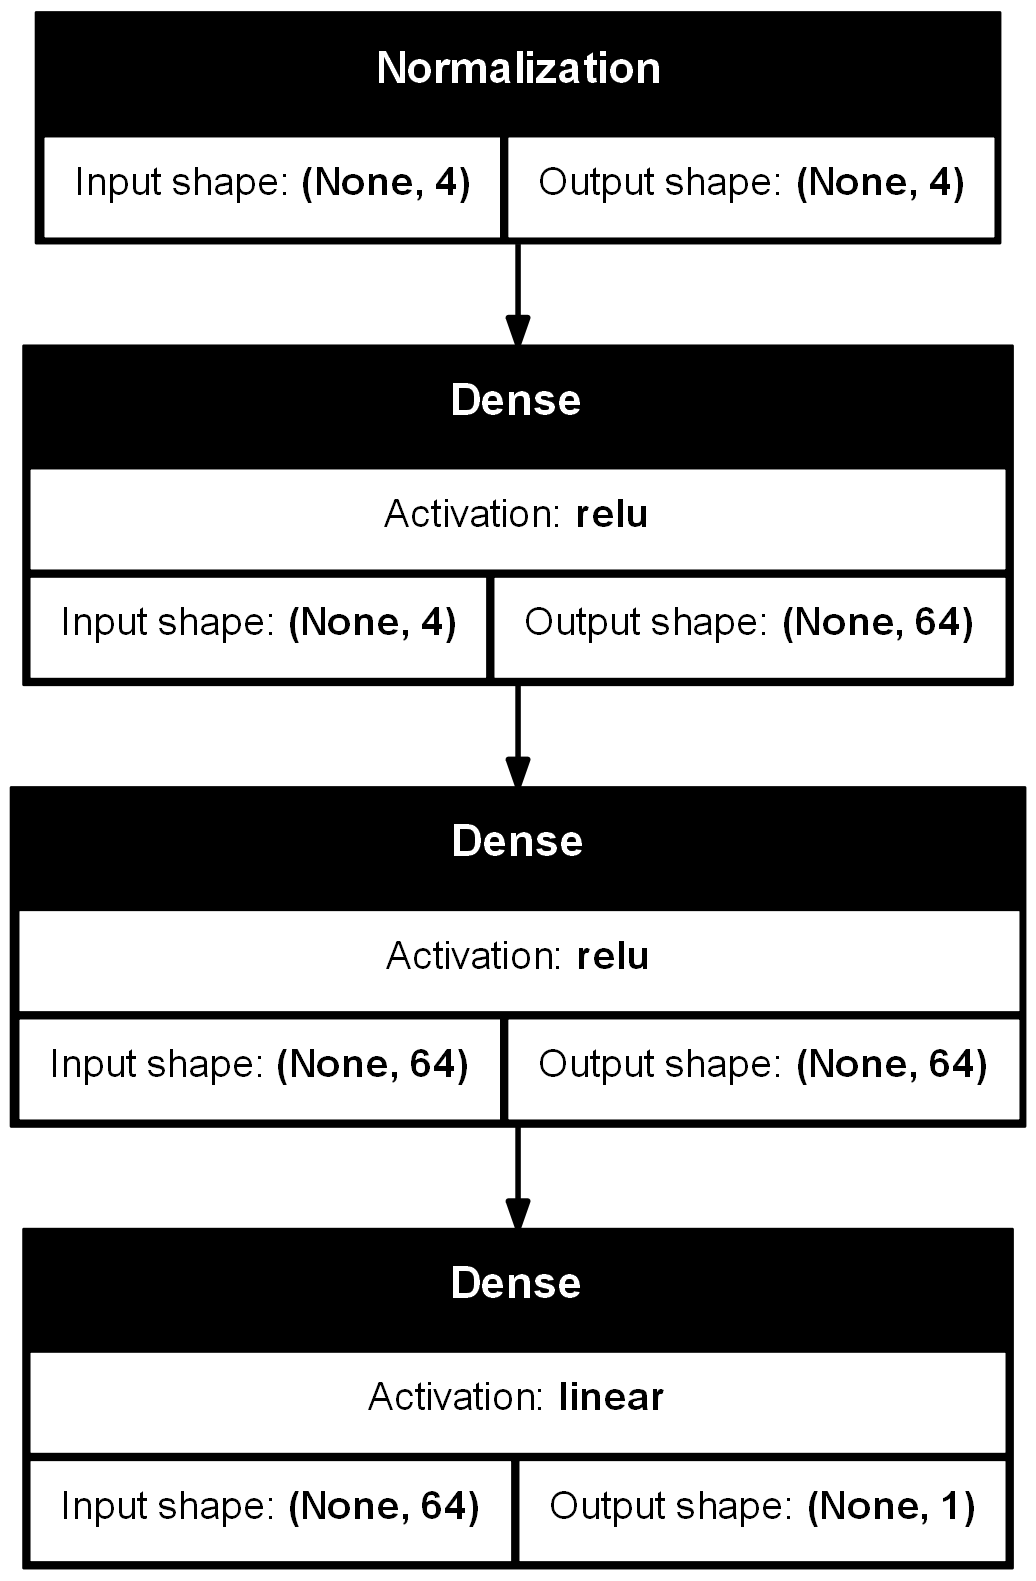
\includegraphics[width=\linewidth]{images/Results/Neural Net/2HL/structure.png}
      \caption{Neural Network Structure with $2$ Hidden layer}


  \end{minipage}
\end{figure}

\begin{figure}[H]
  \centering
  \begin{minipage}{0.4\textwidth}
      \centering
      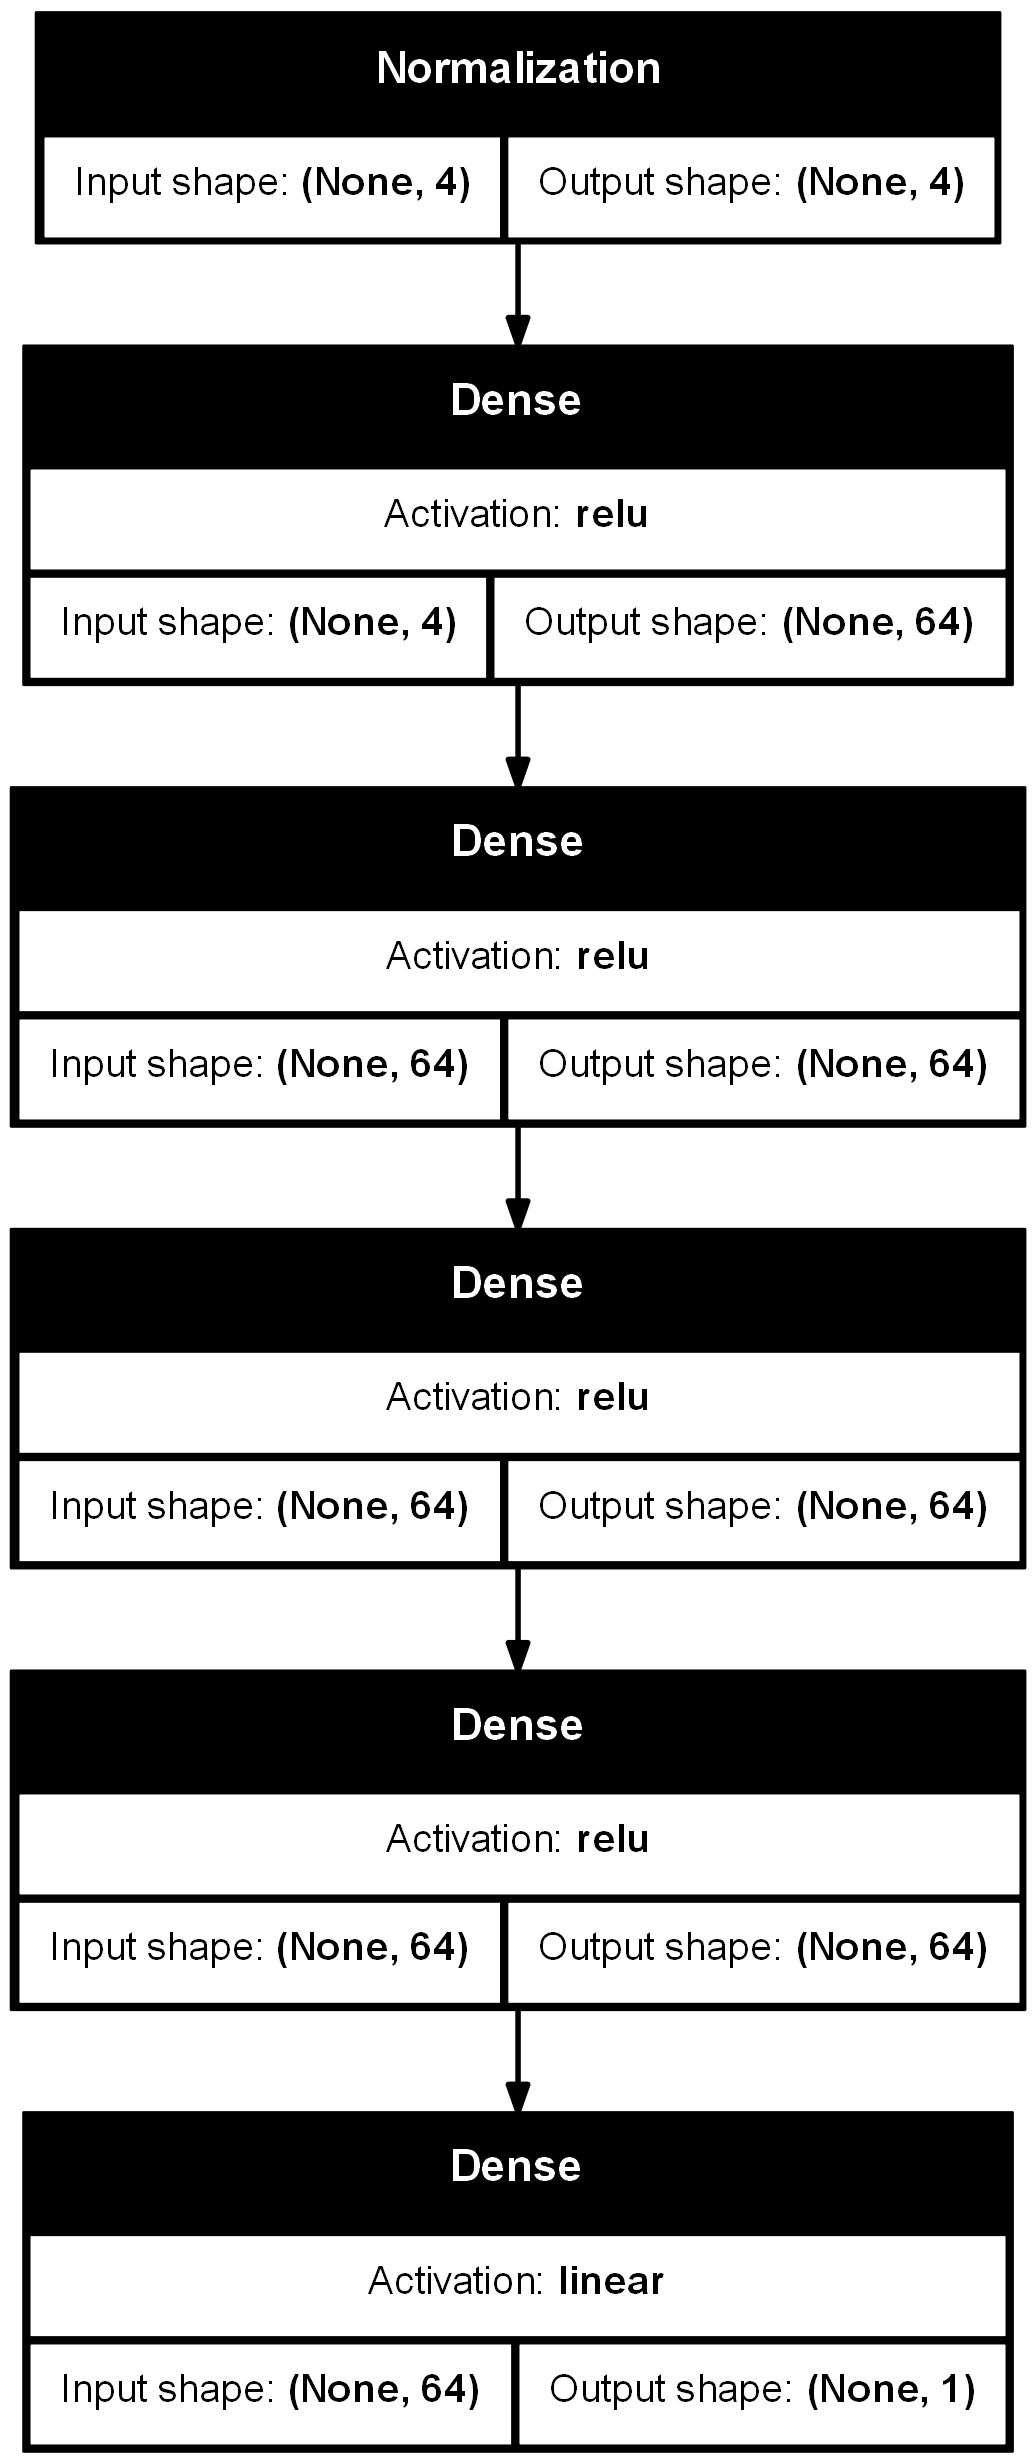
\includegraphics[width=\linewidth]{images/Results/Neural Net/4HL/structure.png}
      \caption{Neural Network Structure with $4$ Hidden layer}
  \end{minipage}
  \hfill
  \begin{minipage}{0.4\textwidth}
      \centering
      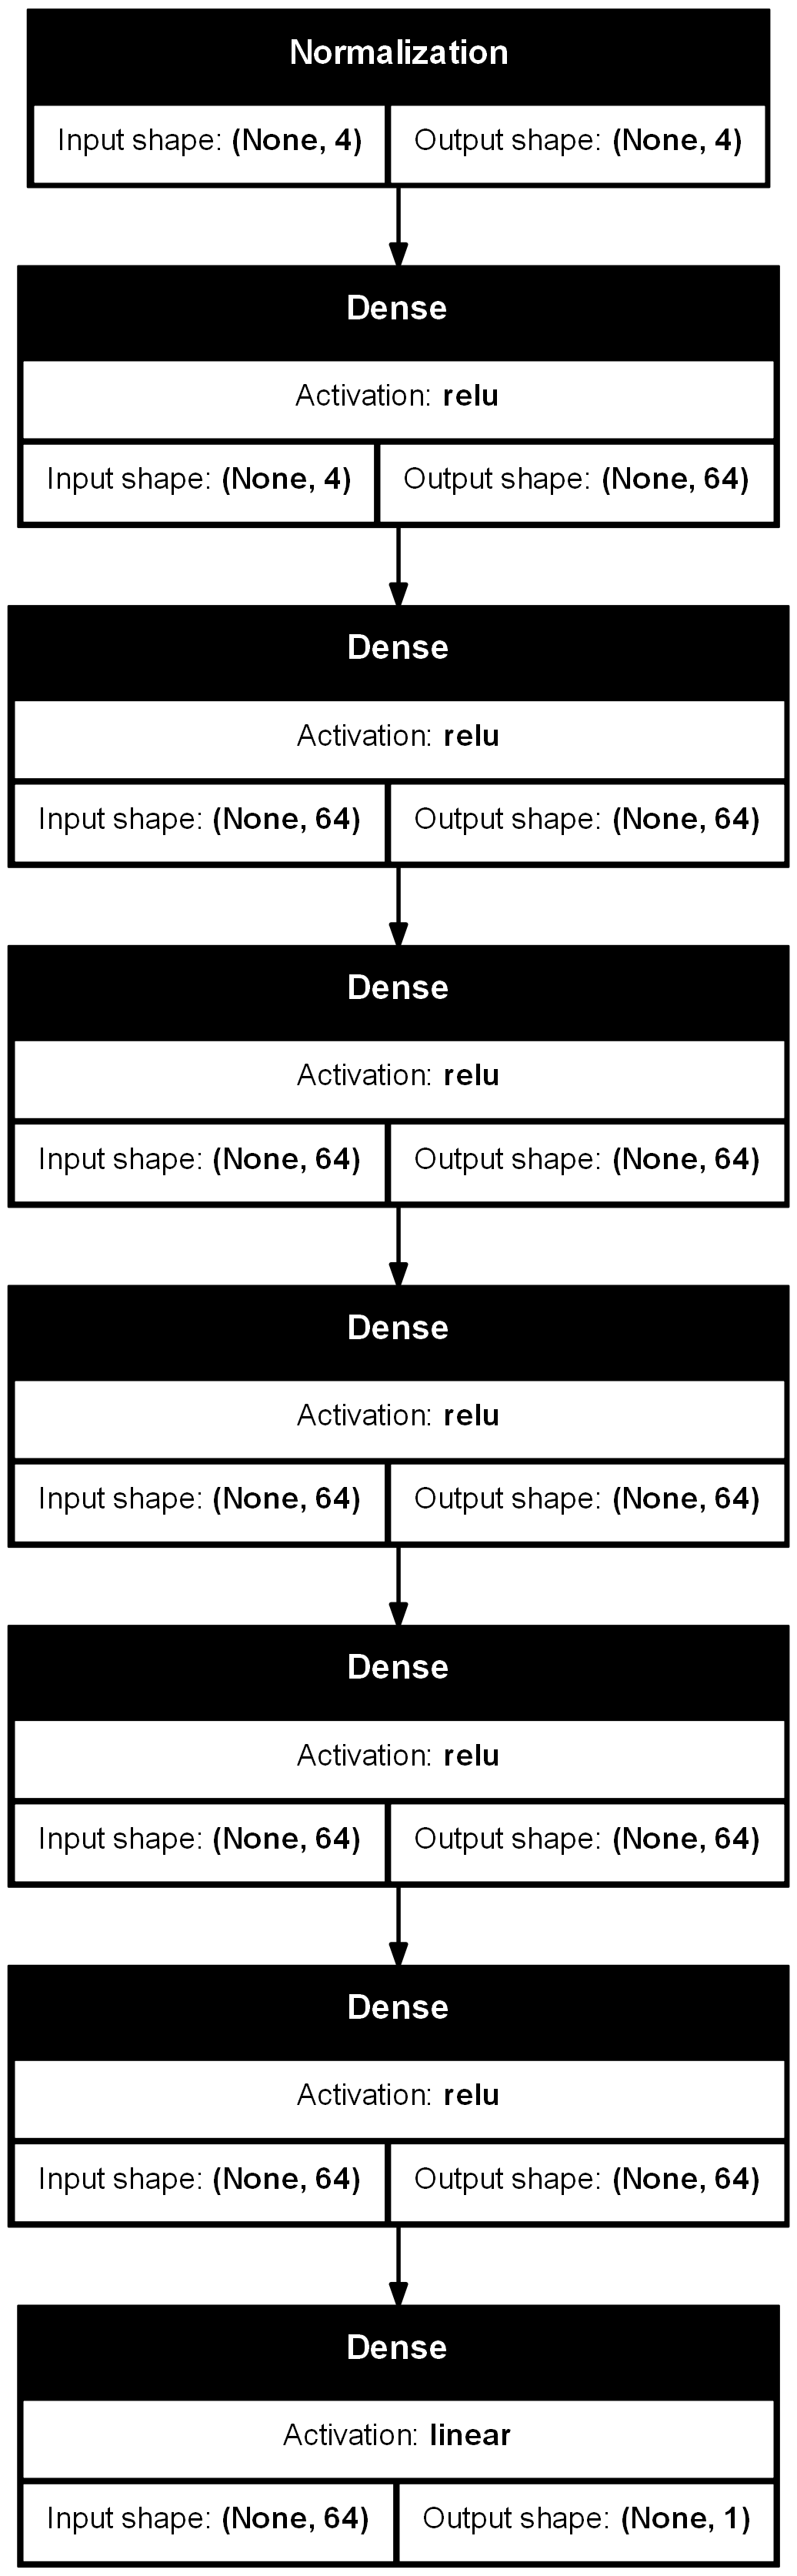
\includegraphics[width=\linewidth]{images/Results/Neural Net/6HL/structure.png}
      \caption{Neural Network Structure with $6$ Hidden layer}
  \end{minipage}
\end{figure}


\subsubsection{Loss Function}

The loss function of choice for this application is the Mean Average
Error described in \autoref{eq:MAE} because it is easy to
interpret as it has the same units as the output variable and is robust
to outliers.

\subsubsection{Optimizer}

The optimizer of choice is Adam which is widely used and considered one
of the best optimizers with a learning rate of 0.01

\subsubsection{Hyper Parameter Tuning}
\label{Hyper-Parameter-Tuning}

Finally, a Hyper tuned model is constructed using the HyperBand
Algorithm. The model is free to choose the following hyperparameters:

\begin{itemize}
\item
  The Number of Hidden layers between 1 and 10
\item
  The number of Neurons for each layer from a discrete set of values
  \[\left\{ 2^{i} \right\}, \ with\ i = 1,2,\ldots ,10\]
\item
  The activation function of each layer with the choices being ReLu,
  tanh, Leaky ReLu
\item
  The learning rate of the optimizer
\end{itemize}

The structure of this model is not known at this phase as it is a
product of the optimization process. This is why it will be presented in
the results section.

The results of the Neural networks are presented in \autoref{neural-network-prediction-results}
    \chapter{Αποτελέσματα}
\label{results}
\chapterprecis{
Το κεφάλαιο των Αποτελεσμάτων μελετά τα δυναμικά χαρακτηριστικά πτερυγισμού \textlatin{(flutter)} του φτερού \textlatin{ASW28}. Επιπλέον, παρουσιάζονται τα αποτελέσματα των τεχνικών βελτιστοποίησης που εφαρμόστηκαν. Τέλος, αποδεικνύεται η δυνατότητα που έχουν τα Νευρωνικά Δίκτυα να προβλέπουν την ταχύτητα πτερυγισμού του φτερού.}


\section{Ανάλυση Ιδιομορφών}
\label{modal-analysis}

Για μια καλύτερη κατανόηση των τρόπων με τους οποίους ταλαντώνεται ή πτέρυγα, πραγματοποιείται μια απλή ανάλυση ιδιομορφών. Οι ιδιομορφές και τα ιδιοδιανύσματα που προκύπτουν από αυτήν την ανάλυση είναι εκείνα που θα προέκυπταν σε μια ανάλυση πτερυγιμού για μηδενική ταχύτητα αέρα. Οι πρώτες 6 ιδιομορφές του φτερού παρουσιάζονται στο \autoref{fig:asw28modes}:


\begin{figure}[H]
  \centering
  \subfloat[\textlatin{Mode 1},\quad $f = 1.518 Hz$]{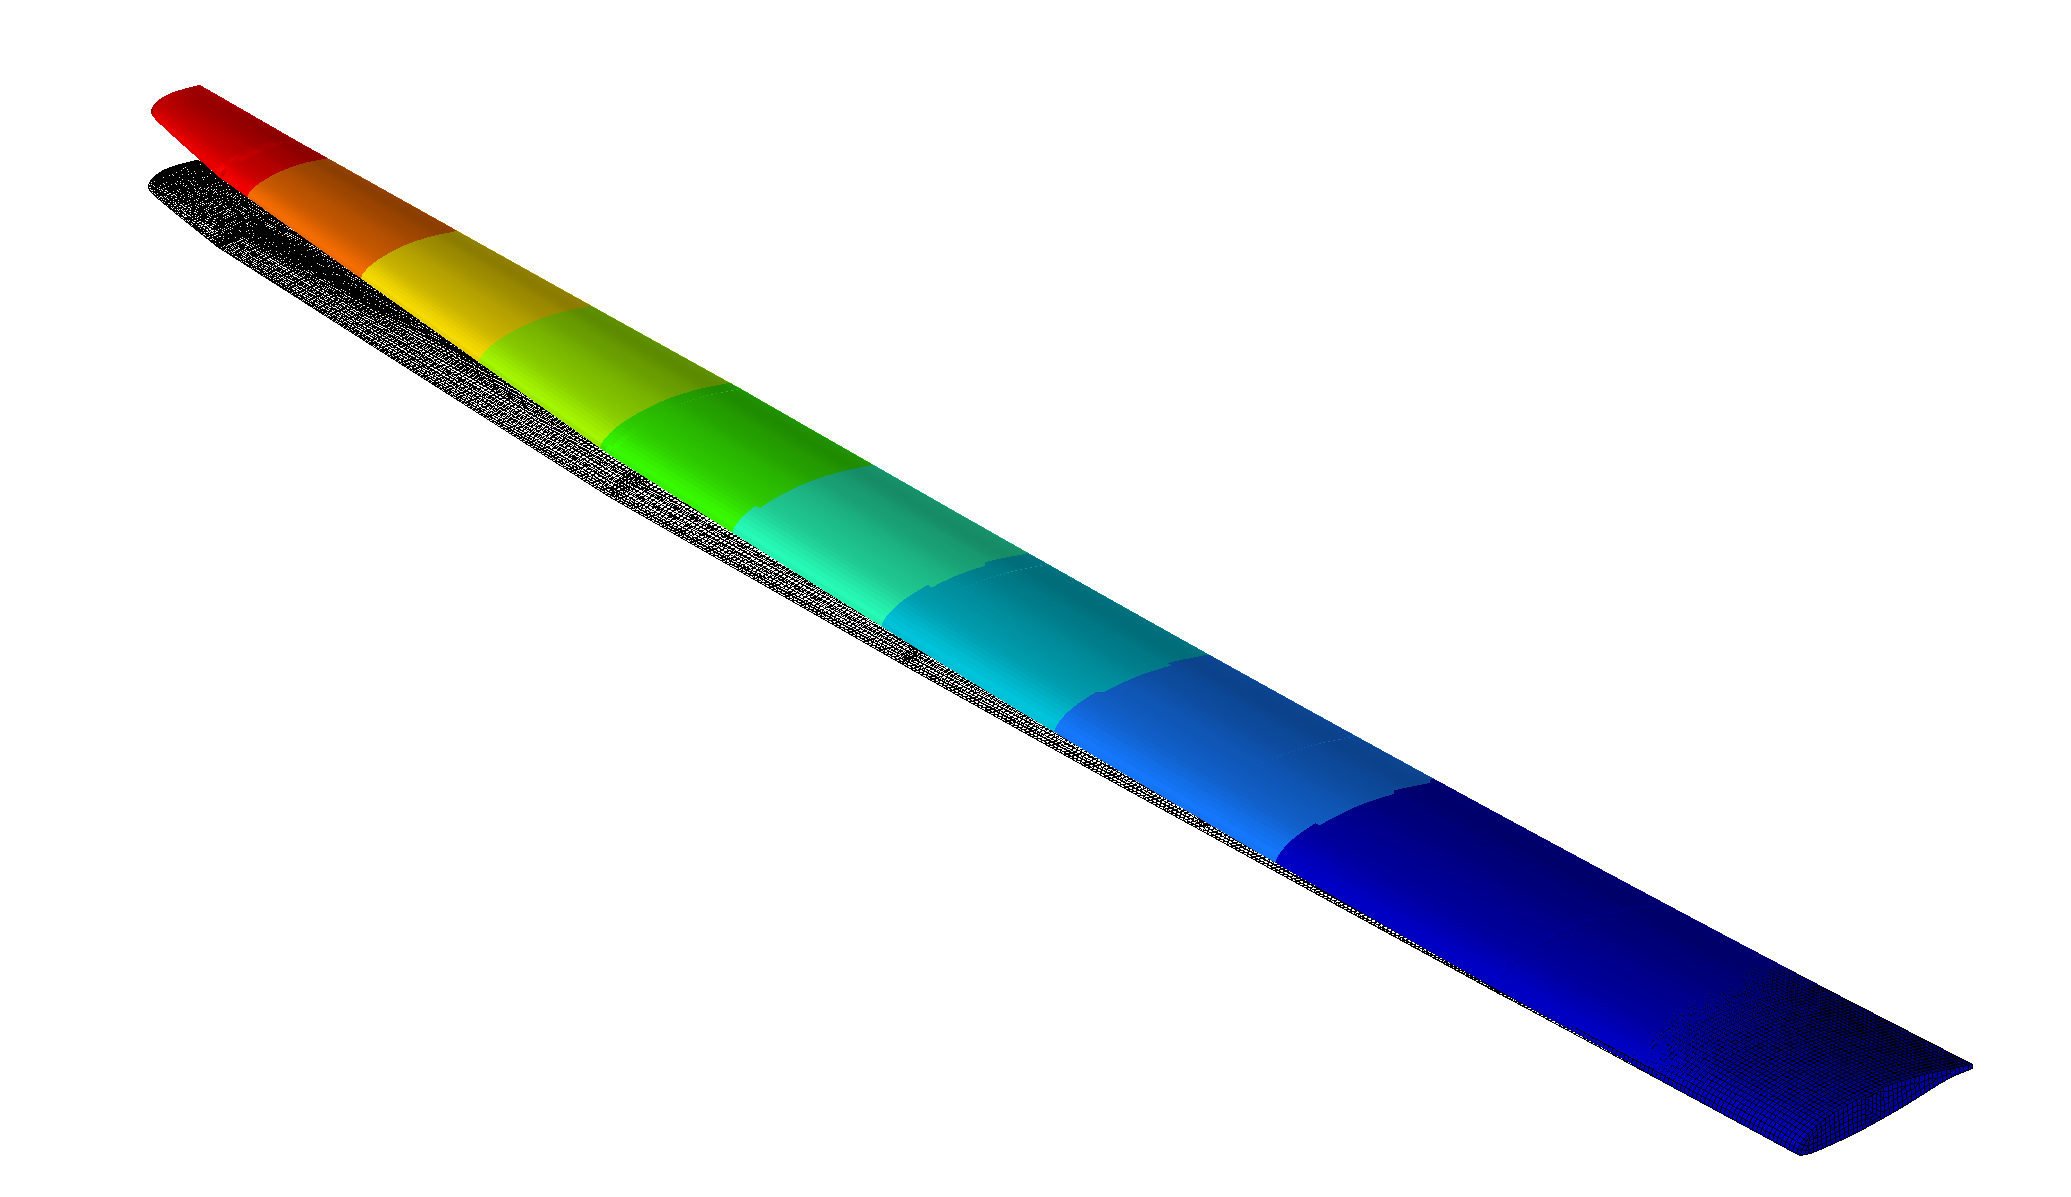
\includegraphics[width=0.5\textwidth]{mode1_1.518Hz.png}}
  \subfloat[\textlatin{Mode 2},\quad $f = 2.704 Hz$]{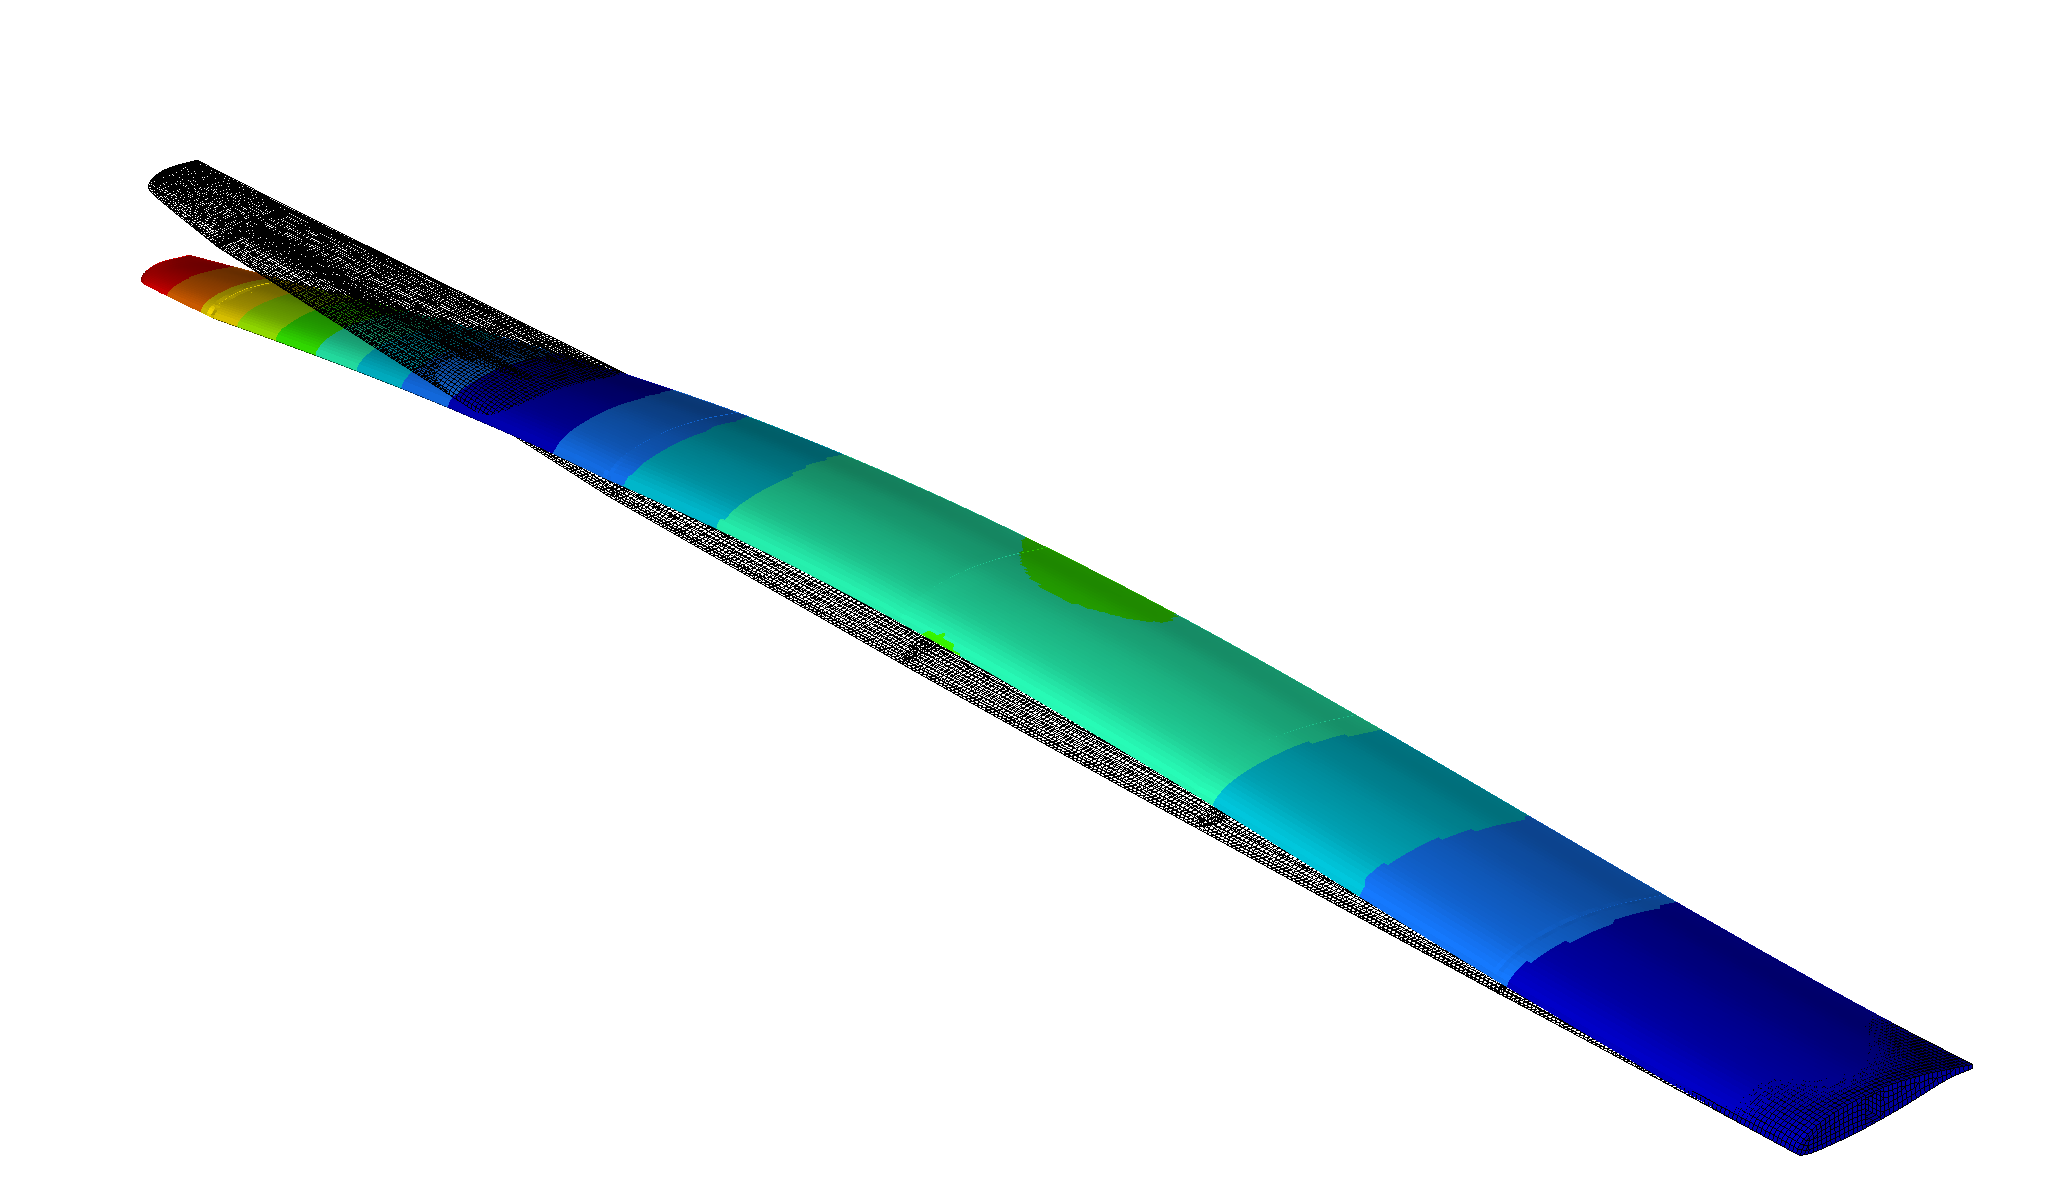
\includegraphics[width=0.5\textwidth]{mode2_7.042Hz.png}}\\
  \subfloat[\textlatin{Mode 3},\quad $f = 7.061 Hz$]{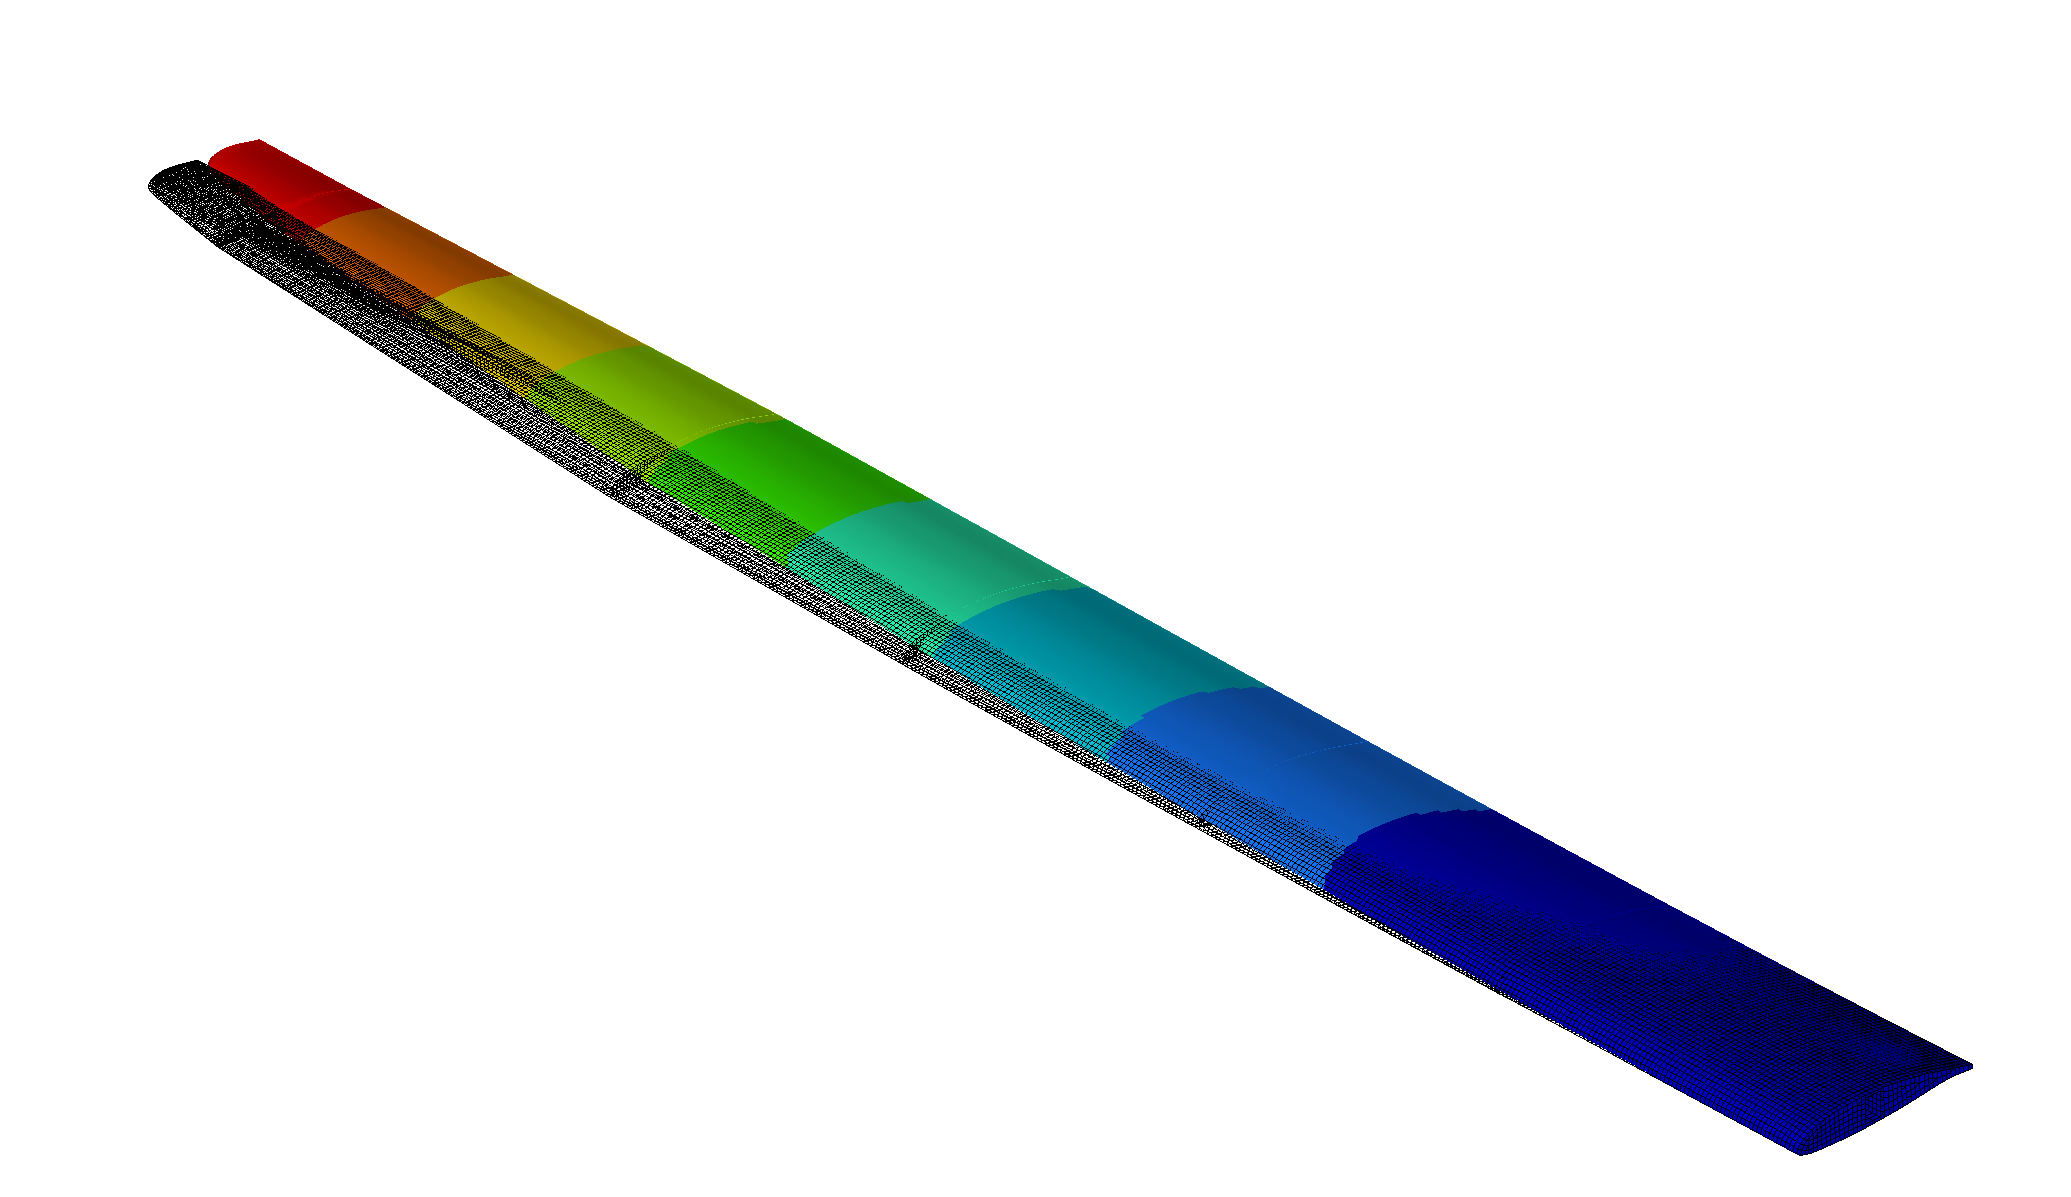
\includegraphics[width=0.5\textwidth]{mode3_7.061Hz.png}} 
  \subfloat[\textlatin{Mode 4},\quad $f = 17.38 Hz$]{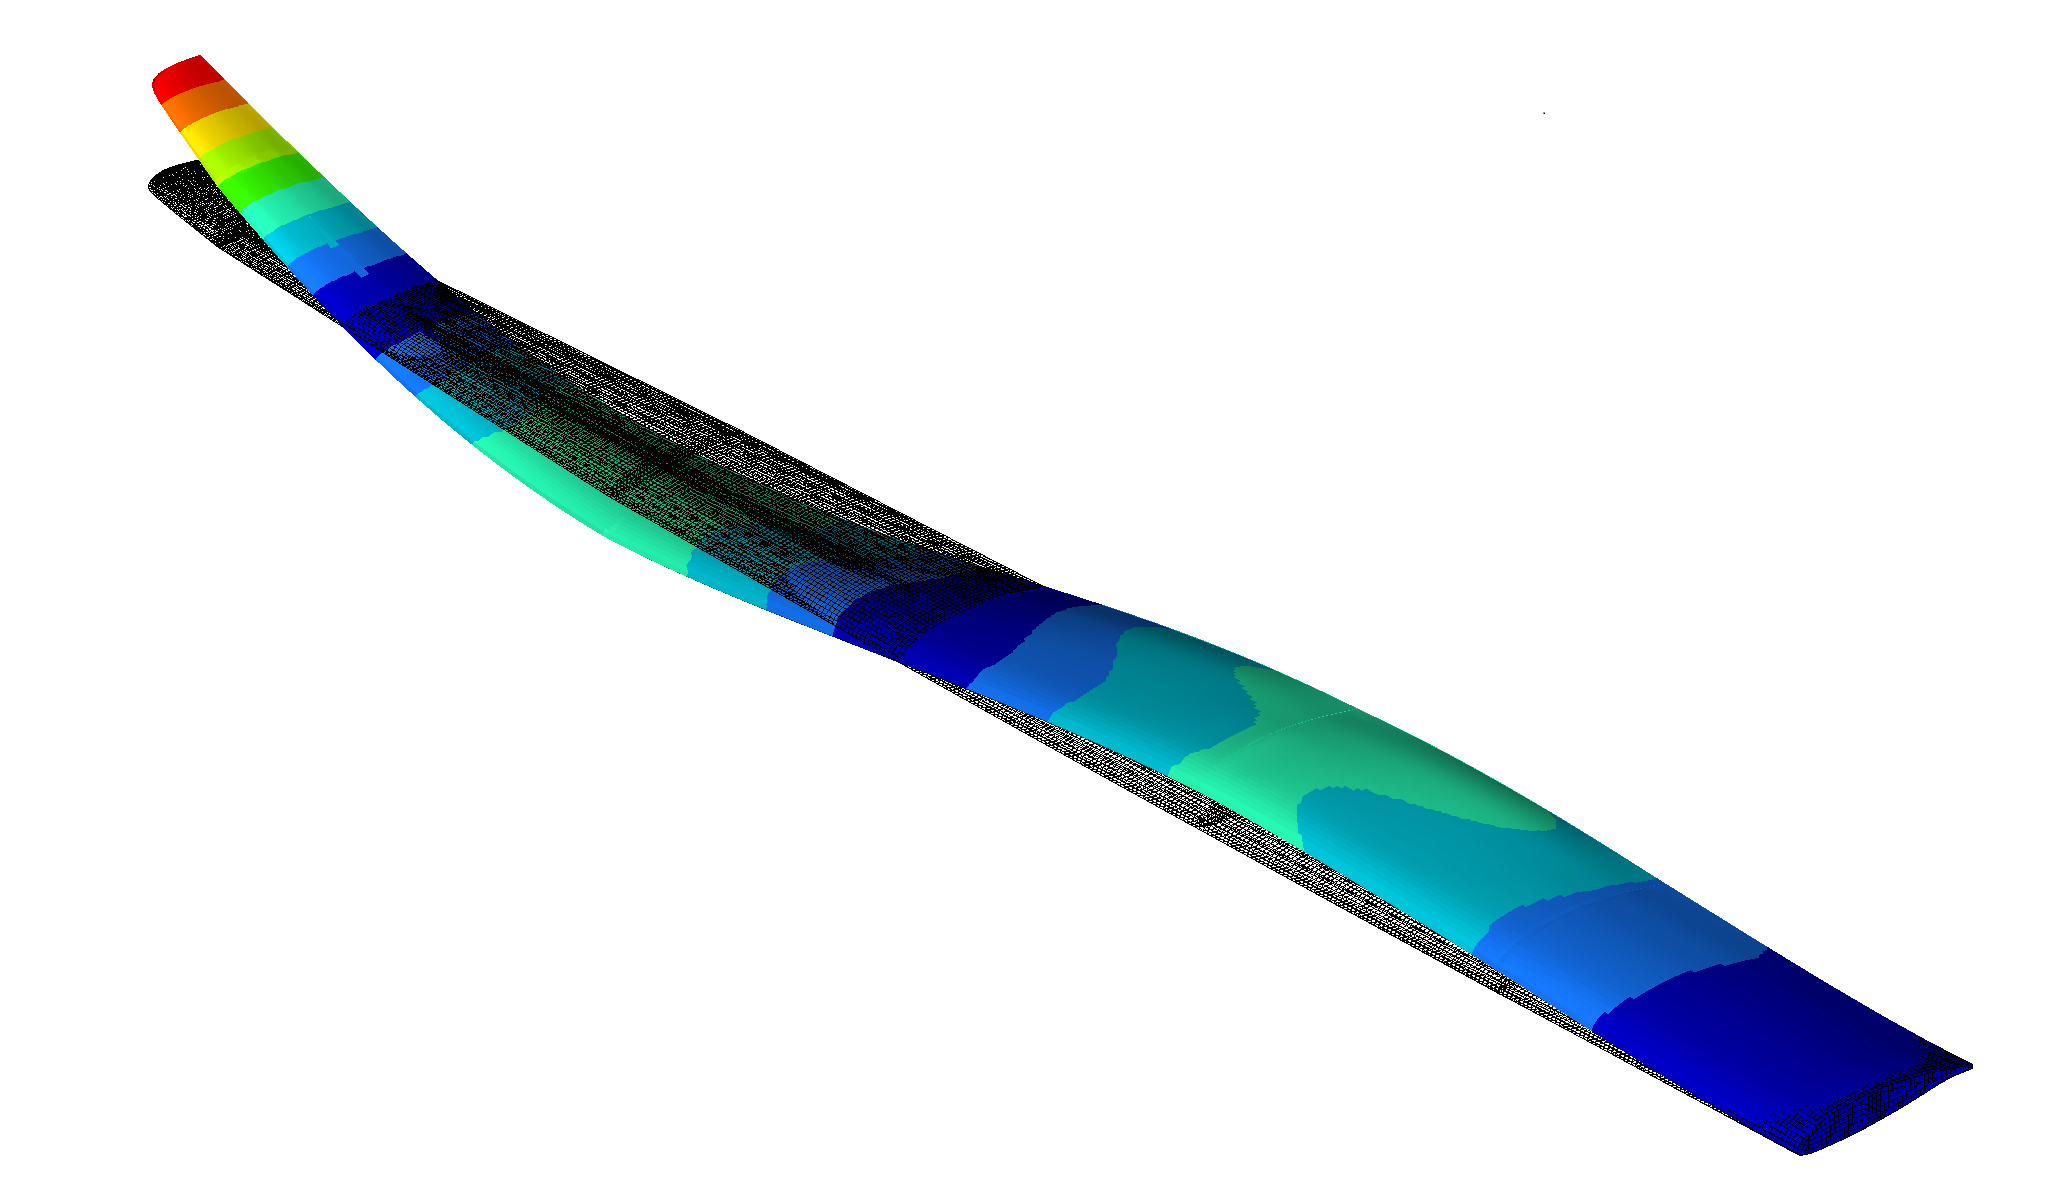
\includegraphics[width=0.5\textwidth]{mode4_17.386Hz.png}}\\
  \subfloat[\textlatin{Mode 5},\quad $f = 30.02 Hz$]{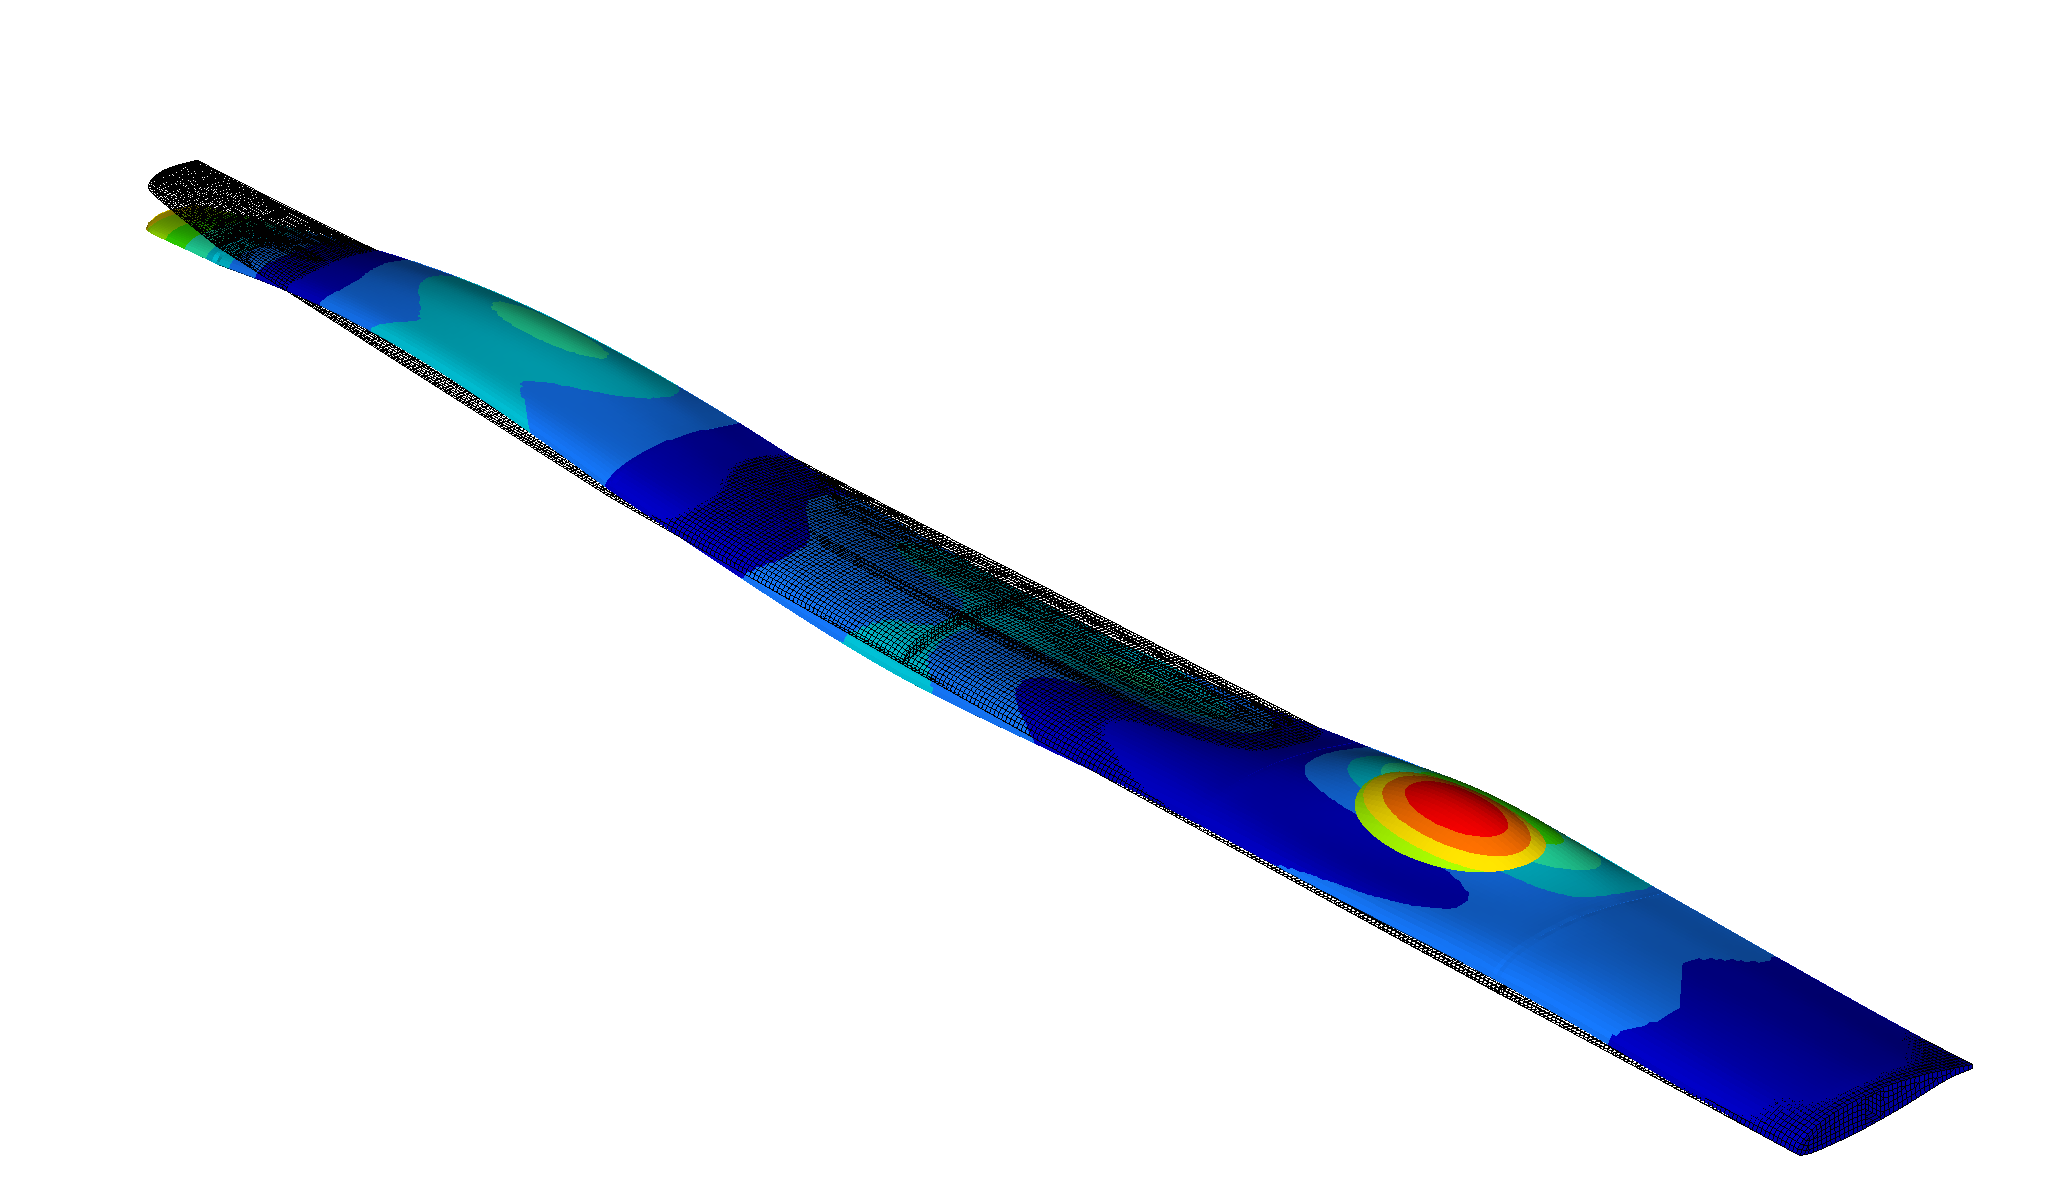
\includegraphics[width=0.5\textwidth]{mode5_30.0168Hz.png}}
  \subfloat[\textlatin{Mode 6},\quad $f = 33.99 Hz$]{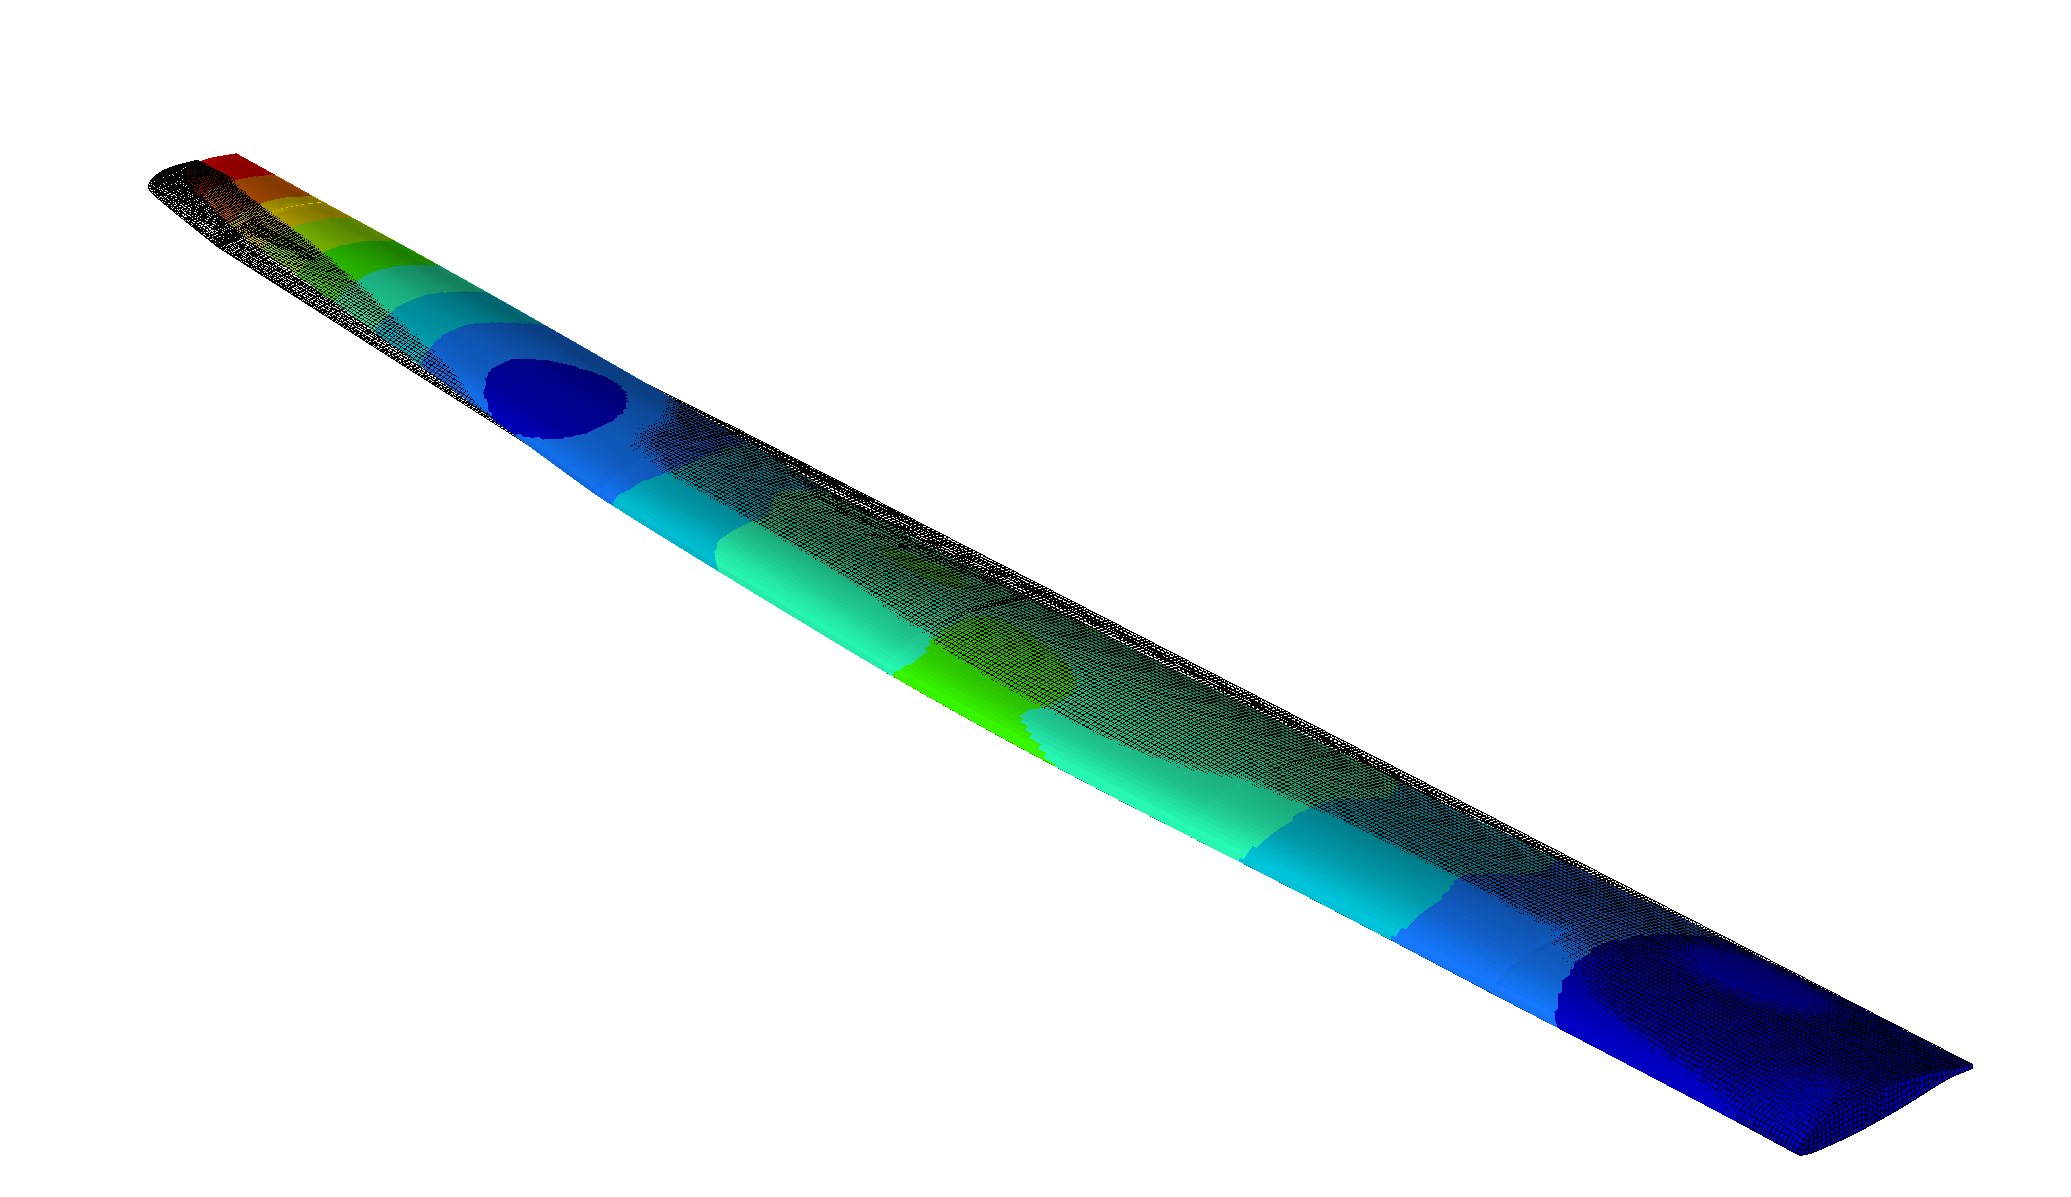
\includegraphics[width=0.5\textwidth]{mode6 33.998Hz.png}}
  \caption{Ο πρώτες 6 ιδιομορφές του φτερού \textlatin{ASW 28}}
  \label{fig:asw28modes}
\end{figure}

Από το \autoref{fig:asw28modes} μπορούν να παρατηρηθούν τα εξής:

\begin{itemize}
\item
  Η πρώτη ιδιομορφή έχει ιδιαίτερα χαμηλή ιδιοσυχνότητα, υποδεικνύοντας ότι το φτερό είναι αρκετά εύκαμπτο σε αυτήν την κατεύθυνση.
\item
  Οι ιδιομορφές 1, 2, 4 και 5 είναι όλες καμπτικές γύρω από τον άξονα $x$, 
  με αυξανόμενο αριθμό κόμβων (σταθερών σημείων) στο φτερό.

  \begin{itemize}
  \item
    Η ιδιομορφή 1 είναι η πιο απλή με ένα μόνο κόμβο στη ρίζα του φτερού. Καθώς η ιδιοσυχνότητα αυξάνεται, αυξάνεται και η πολυπλοκότητα της καμπτικής κίνησης καθώς και ο αριθμός των κόμβων.
  \item
    Η ιδιομορφή 2 έχει δύο κόμβους, ένα στη ρίζα του φτερού και έναν περίπου στα τρία τέταρτα του εκπετάσματος της πτέρυγας.
  \item
    Η ιδιομορφή 4 έχει τρεις κόμβους, ένα στη ρίζα του φτερού, ένα στη μέση και έναν περίπου στο 5/6 του εκπετάσματος της πτέρυγας.
  \item
    Η ιδιομορφή 5 έχει τέσσερις κόμβους κατανεμημένους κατά μήκος του εκπετάσματος της πτέρυγας, αλλά παρουσιάζει επίσης κάποιες ενδείξεις ταλάντωσης πλάκας στην άνω επιφάνεια της πτέρυγας, κοντά στη ρίζα, όπου τα \textlatin{ribs} είναι πιο απομακρυσμένα και υπάρχει ένα μεγάλο τμήμα επιφάνειας του φτερού χωρίς στήριξη.
  \end{itemize}
\item
  Οι ιδιομορφές 3 και 6 είναι καμπτικές γύρω από τον άξονα $z$. Η ιδιομορφή 3 έχει μόνο έναν κόμβο, ενώ η ιδιομορφή 6 έχει δύο.
\end{itemize}


\section{Αρχική Ανάλυση Πτερυγισμού}
\label{initial-flutter-analysis}

Εφαρμόζοντας στο μοντέλο τη μεθοδολογία που αναπτύχθηκε στην \autoref{asw-28-main-composite-wing-model}, προκύπτουν τα εξής αποτελέσματα:


\begin{figure}[H]
    \centering
    \includesvg[width=\textwidth]{initialFlutter.svg}
    \caption{Αρχικό διάγραμμα πτερυγισμού για τις 4 πρώτες ιδιομορφές.}
    \label{fig:initflutter}
\end{figure}


\begin{figure}[H]
    \centering
    \includesvg[width=\textwidth]{InitialFlutterMode3.svg}
    \caption{Διάγραμμα πτερυγισμού για την 3\textsuperscript{η} ιδιομορφή}
    \label{fig:initfluttermode3}
\end{figure}

Από τα Σχήματα \ref{fig:initflutter} και \ref{fig:initfluttermode3} μπορούμε να δούμε ότι το \textlatin{Flutter} συμβαίνει στην
3\textsuperscript{η} ιδιομορφή με:

\begin{equation}
V_{flutter} = 94.11\ m/s
\end{equation}

Παρατηρείται ότι η 1\textsuperscript{η} ιδιομορφή είναι πολύ πιθανό να αποκλίνει επίσης περίπου στην ίδια ταχύτητα, αν και η απόσβεσή της δεν αλλάζει πρόσημο. Η απότομη αύξηση της απόσβεσης σε μια τιμή κοντά στο μηδέν (αλλά ακόμη αρνητική), μαζί με τη μείωση της ιδιοσυχνότητας σχεδόν στο μηδέν, υποδεικνύουν την ύπαρξη στατικής αεροελαστικής απόκλισης (\textlatin{aeroelastic divergence}) που δεν καταγράφεται από τον αλγόριθμο. Η συμπεριφορά αυτή είναι αναμενόμενη για πολύ ευκαμπτες πτέρυγες με μεγάλα εκπετάσματα όταν μελετούνται με γραμμική ανάλυση πτερυγισμού, όμως όπως έχουν δείξει μελέτες μέσω μη γραμμικών προσομοιώσεων και πειραμάτων, αυτό δεν αντικατοπτρίζει κατ' ανάγκη την πραγματικότητα, διότι τα μη γραμμικά φαινόμενα υπερισχύουν σε μεγάλες μετατοπίσεις \cite{NonlinearAeroelasticStability}.

\section{Μέθοδος Βελτιστοποίησης \textlatin{Powell}}
\label{powells-optimization-method}

Μετά την εφαρμογή της μεθόδου βελτιστοποίησης \textlatin{Powell} όπως περιγράφεται στήν \autoref{applying-powells-method}, προκύπτουν τα εξής αποτελέσματα:

\subsubsection{Περίπτωση 1:}

Αυτή ήταν η πρώτη αντικειμενική συνάρτηση που διατυπώθηκε στην εξίσωση \eqref{eq:objpowell1}, καθώς ορίζει ένα πιο ολοκληρωμένο πρόβλημα βελτιστοποίησης. Η βελτιστοποίηση ολοκληρώθηκε με μερική επιτυχία. Τα αποτελέσματα παρουσιάζονται στο \autoref{fig:ValueofobjectivefunctionthroughouttheoptimizationScenario1}:

\begin{figure}[H]
    \centering
    \includesvg[width=\textwidth]{Objective1.svg}
    \caption{Τιμή της αντικειμενικής συνάρτησης κατά τη διάρκεια της βελτιστοποίησης (Περίπτωση 1)}
    \label{fig:ValueofobjectivefunctionthroughouttheoptimizationScenario1}
\end{figure}

\begin{figure}[H]
    \centering
    \includesvg[width=\textwidth]{Variables1.svg}
    \caption{Τιμή κάθε μεταβλητής βελτιστοποίησης κατά τη διάρκεια της βελτιστοποίησης (Περίπτωση 1)
    }
\end{figure}

Όπως φαίνεται ο αλγόριθμος αποτυγχάνει να βελτιώσει την αντικειμενική συνάρτηση πέρα από το αρχικό σημείο. Στην πρώτη επανάληψη, ο αλγόριθμος προσπαθεί να μειώσει τη μάζα της πτέρυγας μειώνοντας το πάχος των στρωμάτων κατά ένα δέκατο του χιλιοστού, αλλά η ταχύτητα πτερυγισμού μειώνεται υπερβολικά και επιβάλλεται η ποινή, με αποτέλεσμα μια πολύ υψηλή τιμή της αντικειμενικής συνάρτησης.

Από εκείνο το σημείο, ο αλγόριθμος πειραματίζεται με μεγαλύτερες τιμές πάχους, οι οποίες φυσικά οδηγούν σε μεγαλύτερη μάζα, αλλά με αρκετά υψηλή ταχύτητα πτερυγισμού ώστε να μην επιβληθεί η ποινή.

Τελικά, ο αλγόριθμος μειώνει το πάχος των στρωμάτων σταδιακά μέχρι να φτάσει στο αρχικό πάχος.

Ο αλγόριθμος δεν αντιλαμβάνεται ότι αλλάζοντας πρώτα τις γωνίες των στρωμάτων ώστε η ταχύτητα πτερυγισμού να αυξηθεί και στη συνέχεια μειώνοντας το πάχος, η ταχύτητα πτερυγισμού παραμένει αρκετά υψηλή ώστε να μην επιβληθεί η ποινή ενώ ταυτόχρονα μειώνεται η μάζα. Αυτή είναι μια περίπλοκη λύση, καθώς οι γωνίες δεν επηρεάζουν άμεσα τη μάζα, αλλά μόνο την ταχύτητα πτερυγισμού. Αν ο αλγόριθμος είχε εξερευνήσει καλύτερα τις γωνίες ενώ βρισκόταν στη ζώνη ποινής, θα μπορούσε να είχε αυξήσει την ταχύτητα του πτερυγισμού επαρκώς για να βγει από τη ζώνη ποινής και τελικά να βρει μια καλύτερη λύση. Δυστυχώς, αυτή η συμπεριφορά είναι αρκετά σύνθετη και ξεπερνά τις δυνατότητες αυτού του σχετικά απλού αλγορίθμου.

Τα αποτελέσματα της ανάλυσης πτερυγισμού της τελικής λύσης αυτού του αλγορίθμου παρουσιάζονται στα σχήματα \ref{fig:FlutteranalysisplotsfromPowellsmethodScenario1} και \ref{fig:Mode3FlutteranalysisPowellsmethodScenario1}:


\begin{figure}[H]
    \centering
    \includesvg[width=\textwidth]{Flutter1.svg}
    \caption{Διαγράμματα ανάλυσης πτερυγισμού από τη μέθοδο του \textlatin{Powell}. (Περίπτωση 1)}
    \label{fig:FlutteranalysisplotsfromPowellsmethodScenario1}
\end{figure}

Η πρώτη ιδιομορφή που παρουσιάζει απόκλιση είναι η ιδιομορφή 3, η οποία απεικονίζεται μόνη της στο επόμενο σχήμα ώστε να φανεί καθαρά πότε αλλάζει πρόσημο η απόσβεση.

\begin{figure}[H]
    \centering
    \includesvg[width=\textwidth]{Flutter1Mode3.svg}
    \caption{Ανάλυση πτερυγισμού της 3\textsuperscript{ης} ιδιομορφής με τη μέθοδο του \textlatin{Powell}. (Περίπτωση 1)}
    \label{fig:Mode3FlutteranalysisPowellsmethodScenario1}
\end{figure}

Η ταχύτητα με την οποία η ιδιομορφή αυτή αποκλίνει για πρώτη φορά είναι η ταχύτητα πτερυγισμού και στην προκειμένη περίπτωση:


\begin{equation}
V_{flutter} = 99.48\ m/s
\end{equation}

\subsubsection{Περίπτωση 2:}

Για να επιτευχθεί ένα καλύτερο αποτέλεσμα, χρησιμοποιείται η απλοποιημένη αντικειμενική συνάρτηση της εξίσωσης \eqref{eq:objpowell2}. 
Αυτή τη φορά, ο αλγόριθμος εξερευνά το χώρο των πιθανών λύσεων με μεγαλύτερη επιτυχία. Τα αποτελέσματα παρουσιάζονται στο \autoref{fig:objpowell2}:


\begin{figure}[H]
    \centering
    \includesvg[width=\textwidth]{Objective2.svg}
    \caption{Τιμή της αντικειμενικής συνάρτησης κατά τη διάρκεια της βελτιστοποίησης (Περίπτωση 2)}
    \label{fig:objpowell2}
\end{figure}

\begin{figure}[H]
  \centering
  \includesvg[width=\textwidth]{Variables2.svg}
  \caption{Τιμή κάθε μεταβλητής βελτιστοποίησης κατά τη διάρκεια της βελτιστοποίησης (Περίπτωση 2)}
\end{figure}

Παρατηρείται από το \autoref{fig:objpowell2} ότι η αντικειμενική συνάρτηση, η οποία τώρα αποσκοπεί στην ελαχιστοποίηση της αρνητικής ταχύτητας πτερυγισμού, έχει βελτιωθεί σημαντικά.

Επιπλέον, σύμφωνα με τον ορισμό αυτού του προβλήματος, η μεταβλητή πάχους παραμένει σταθερή και ίση με την αρχική τιμή των $0.5 mm$. Αυτό σημαίνει ότι ενώ η ταχύτητα πτερυγισμού αυξάνεται σημαντικά, η μάζα παραμένει σταθερή.

Τα διαγράμματα πτερυγισμού για την βέλτιστη λύση αυτής της μεθόδου παρουσιάζονται στα σχήματα \ref{fig:PowerllFlutterPlotScenario2} και \ref{fig:PowerllFlutter3PlotScenario2} .


\begin{figure}[H]
    \centering
    \includesvg[width=\textwidth]{Flutter2.svg}
    \caption{Διαγράμματα ανάλυσης πτερυγισμού  από τη μέθοδο του \textlatin{Powell}. (Περίπτωση 2)}
    \label{fig:PowerllFlutterPlotScenario2}
\end{figure}


\begin{figure}[H]
    \centering
    \includesvg[width=\textwidth]{Flutter2Mode3.svg}
    \caption{Ανάλυση πτερυγισμού της 3\textsuperscript{ης} ιδιομορφής με τη μέθοδο του \textlatin{Powell}. (Περίπτωση 2)}
    \label{fig:PowerllFlutter3PlotScenario2}

\end{figure}

Για άλλη μια φορά, η πρώτη ιδιομορφή που αποκλίνει είναι η ιδιομορφή 3. Αυτή τη φορά όμως, η ταχύτητα είναι πολύ μεγαλύτερη από πριν.

\begin{equation}
V_{flutter} = 175.28\ m/s
\end{equation}

Οι ιδιομορφές 1 και 4 αποκλίνουν επίσης στα $267.09$ και $177.14 m/s$ αντίστοιχα. Όπως είναι προφανές, αυτή είναι μια εξαιρετική βελτίωση της ταχύτητας πτερυγισμού του φτερού σε σχέση με την αρχική λύση, χωρίς επιπλέον υλικό και άρα με την ίδια μάζα με το αρχικό φτερό.

Το διάνυσμα που δίνει τη βέλτιστη λύση είναι:

\begin{equation}
{\vec{\mathbf{x}}}_{opt} = \lbrack 0.0005,90, - 58, - 59\rbrack^{T}
\end{equation}


\section{Βελτιστοποίηση με τη μέθοδο Γενετικών Αλγορίθμων}
\label{genetic-algorithm-optimization}

Μετά την εφαρμογή της μεθόδου γενετικών αλγορίθμων όπως περιγράφεται στήν \autoref{applying-the-genetic-algorithm}, προκύπτουν τα εξής αποτελέσματα:

\begin{figure}[H]
    \centering
    \includesvg[width=\textwidth]{fitness.svg}
    \caption{Εξέλιξη του \textlatin{fittness fucntion} της καλύτερης λύσης κάθε γενιάς κατά τη διαδικασία βελτιστοποίησης}
    \label{fig:fitnessevolution}
\end{figure}


\begin{figure}[H]
    \centering
    \includesvg[width=\textwidth]{genes.svg}
    \caption{Εξέλιξη των τιμών των γονιδίων κατά τη διάρκεια της διαδικασίας βελτιστοποίησης.}
\end{figure}



Από το \autoref{fig:fitnessevolution}, όπου απεικονίζεται η καλύτερη λύση που βρέθηκε μέχρι στιγμής σε κάθε γενιά, παρατηρείται ότι και οι δύο στόχοι βελτιώνονται μέχρι το τέλος της βελτιστοποίησης, παρόλο που αυτοί είναι αντιφατικοί μεταξύ τους. Από τα αρχεία καταγραφής της βελτιστοποίησης, η καλύτερη λύση έχει τα εξής χαρακτηριστικά:


\begin{equation}
V_{flutter} = 214.69\ m/s,\quad Mass = 45.1\ kg
\end{equation}

Οι τιμές των γονιδίων που οδηγούν στη βέλτιστη λύση είναι:


\begin{equation}
t = 0.0003\ mm,\ \ \vartheta_{1} = 43{^\circ},\ \ \vartheta_{2} = 56{^\circ},\ \ \vartheta_{3} = 76{^\circ}
\end{equation}

Το διάγραμμα πτερυγισμού  για αυτήν τη λύση παρουσιάζεται στο \autoref{fig:FlutterPlotfromGeneticAlgorithm}:

\begin{figure}[H]
    \centering
    \includesvg[width=\textwidth]{FlutterPlot4modes.svg}
    \caption{Διάγραμμα πτερυγισμού  από τον αλγόριθμο γενετικής βελτιστοποίησης.}
    \label{fig:FlutterPlotfromGeneticAlgorithm}
\end{figure}

\begin{figure}[H]
    \centering
    \includesvg[width=\textwidth]{FlutterPlotmode1.svg}
    \caption{Διάγραμμα πτερυγισμού της 1\textsuperscript{ης} ιδιομορφής από αλγόριθμο γενετικής βελτιστοποίησης}
    \label{fig:GAflutterMode1}
\end{figure}

Αν και η λύση που προκύπτει από τη μέθοδο των γενετικών αλγορίθμων φαίνεται ιδανική, εξετάζοντας το \autoref{fig:GAflutterMode1} μπορούμε να δούμε ότι πριν από την αναφερόμενη ταχύτητα πτερυγισμού των $214 m/s$, η απόσβεση  της 1\textsuperscript{ης} ιδιομορφής αλλάζει σημαντικά στα $110 m/s$ και η ιδιοσυχνότητα μειώνεται στο μηδέν, το οποίο είναι ένδειξη στατικής αεροελαστικής απόκλισης \textlatin{(static aeroelastic divergence)}. Είναι πιθανό αυτό να μη συμβαίνει στην πραγματικότητα, διότι όπως έχουμε δει σε άλλες μελέτες \cite{NonlinearAeroelasticStability}, όταν το φτερό εκτρέπεται με μεγάλες μετατοπίσεις, τα μη γραμμικά φαινόμενα γίνονται σημαντικά και απαιτούνται μη γραμμικές αναλύσεις στατικής αερολαστικότητας για τον εντοπισμό τέτοιων φαινομένων.

\section{Αποτελέσματα Πρόβλεψης μέσω Νευρωνικών Δικτύων}
\label{neural-network-prediction-results}

Σε αυτή την ενότητα, θα παρουσιαστούν τα αποτελέσματα κάθε Νευρωνικού Δικτύου που αναπτύχθηκε στήν \autoref{flutter-speed-prediction-using-neural-networks}. Παρουσιάζονται τρία βασικά διαγράμματα για την κατανόηση της απόδοσης κάθε δικτύου.

\begin{enumerate}
\def\labelenumi{\arabic{enumi}.}
\item
  Το πρώτο διάγραμμα δείχνει την τιμή της συνάρτησης απώλειας στα δεδομένα εκπαίδευσης και επικύρωσης σε κάθε εποχή της εκπαίδευσης.
\item
  Το δεύτερο διάγραμμα χρησιμοποιείται για την αξιολόγηση της απόδοσης του δικτύου με τη χρήση του διαγράμματος διασποράς \(y_{pred}\ \text{\textlatin{vs}} \ y_{true}\). Ιδανικά, αυτές οι τιμές θα ταυτίζονταν, παράγοντας μια ευθεία γραμμή με γωνία \(45{^\circ}\).
\item
  Το τρίτο διάγραμμα εμφανίζει τις διαφορές ως προς το \(y_{true}\),  \( (y_{true} - y_{pred})\ \text{\textlatin{vs}} \ y_{true} \), διευκολύνοντας την κατανόηση του μεγέθους του σφάλματος καθώς και τυχόν τάσεων που μπορεί να υπάρχουν σε συγκεκριμένες ταχύτητες πτερυγισμού.
\end{enumerate}

\subsection{Εξέταση δεδομένων εκπαίδευσης}
\label{training-data-examination}

Ένας προκαταρκτικός έλεγχος των δεδομένων πραγματοποιείται χρησιμοποιώντας ένα διάγραμμα συσχέτισης \textlatin{(pair plot)}, το οποίο είναι ένα πλέγμα γραφημάτων που επιτρέπει την οπτικοποίηση της σχέσης μεταξύ κάθε ζεύγους μεταβλητών στο σύνολο δεδομένων.


\begin{figure}[H]
    \centering
    \includesvg[width=\textwidth]{DataExploration/pairplot.svg}
    \caption{\textlatin{pair plot} των δεδομένων εκπαίδευσης}
    \label{fig:pairplot}
\end{figure}

Από το \autoref{fig:pairplot} μπορούμε να παρατηρήσουμε τις εξής σχέσεις στα συγκεντρωμένα δεδομένα:

\begin{enumerate}
\def\labelenumi{\arabic{enumi}.}
\item
  Καθώς αυξάνεται το πάχος, αυξάνεται και η προβλεπόμενη ταχύτητα πτερυγισμού.
\item
  Οι γωνίες \(\theta_{1} - \theta_{3}\) έχουν μια ισχυρά μη γραμμική συσχέτιση με την ταχύτητα πτερυγισμού χωρίς εμφανείς τάσεις.
\item
  Κατά μήκος της διαγωνίου των ιστογραμμάτων που αντιπροσωπεύουν τη συσχέτιση μιας μεταβλητής με τον εαυτό της, παρατηρείται ότι τα δεδομένα είναι κατανεμημένα τυχαία και ομοιόμορφα σε όλο το εύρος των πιθανών τιμών.
\end{enumerate}

\subsection{Νευρωνικό Δίκτυο με 1 Κρυφό Στρώμα}\label{hidden-layer-neural-network}


\begin{figure}[H]
  \centering
  \subfloat[\textlatin{training history}]{\includesvg[width=0.5\textwidth]{1HL/traininghistory.svg}} \\
  \subfloat[$Y_{true}$ \textlatin{vs} $Y_{pred}$]{\includesvg[width=0.5\textwidth]{1HL/Ytrue_vs_Ypred.svg}}
  \subfloat[\textlatin{Residuals}]{\includesvg[width=0.5\textwidth]{1HL/Residuals_vs_Ytrue.svg}}

  \caption{Απόδοση Νευρωνικου δικτύου με 1 κρυφό στρώμα}
  \label{fig:1HLNNperf}
\end{figure}

Από το \autoref{fig:1HLNNperf} καθίσταται προφανές ότι αν και αυτό το μοντέλο με μόνο ένα κρυφό στρώμα εκπαιδεύτηκε για 400 \textlatin{epochs}, οι οποίες είναι αρκετές όπως θα φανεί από τα επόμενα αποτελέσματα, το \textlatin{Mean Average Error} των δεδομένων επικύρωσης είναι πολύ μεγάλο για να είναι χρήσιμο το δίκτυο. Η διακύμανση πάνω και κάτω από τη μηδενική γραμμή στο \autoref{fig:1HLNNperf} (γ') είναι πολύ μεγάλη, με πολλά σημεία να υποεκτιμούνται ή να υπερεκτιμούνται κατά περισσότερο από $50 m/s$.


\subsection{Νευρωνικό Δίκτυο με 2 Κρυφά Στρώματα}
\label{hidden-layer-neural-network-1}
\begin{figure}[H]
  \centering
  \subfloat[\textlatin{training history}]{\includesvg[width=0.5\textwidth]{2HL/traininghistory.svg}} \\
  \subfloat[$Y_{true}$ \textlatin{vs} $Y_{pred}$]{\includesvg[width=0.5\textwidth]{2HL/Ytrue_vs_Ypred.svg}}
  \subfloat[\textlatin{Residuals}]{\includesvg[width=0.5\textwidth]{2HL/Residuals_vs_Ytrue.svg}}

  \caption{Απόδοση Νευρωνικου δικτύου με 2 κρυφά στρώματα}
  \label{fig:2HLNNperf}
\end{figure}
Αυτό το μοντέλο εκπαιδεύτηκε για 350 \textlatin{epochs}. Τα 2 κρυφά στρώματα αποδίδουν πολύ καλύτερα από ένα μόνο στρώμα. Το \textlatin{Mean Average Error} στα δεδομένα επικύρωσης στο τέλος της εκπαίδευσης είναι περίπου $7 m/s$. Το μόνο πρόβλημα είναι ότι εξακολουθεί να υπάρχει μεγάλη διακύμανση στις προβλέψεις, όπως φαίνεται από το \autoref{fig:2HLNNperf}.


\subsection{Νευρωνικό Δίκτυο με 4 Κρυφά Στρώματα}
\label{hidden-layer-neural-network-2}

\begin{figure}[H]
  \centering
  \subfloat[\textlatin{training history}]{\includesvg[width=0.5\textwidth]{4HL/traininghistory.svg}} \\
  \subfloat[$Y_{true}$ \textlatin{vs} $Y_{pred}$]{\includesvg[width=0.5\textwidth]{4HL/Ytrue_vs_Ypred.svg}}
  \subfloat[\textlatin{Residuals}]{\includesvg[width=0.5\textwidth]{4HL/Residuals_vs_Ytrue.svg}}

  \caption{Απόδοση Νευρωνικου δικτύου με 4 κρυφά στρώματα}
  \label{fig:4HLNNperf}
\end{figure}

Το νευρωνικό δίκτυο με τέσσερα κρυφά στρώματα εκπαιδεύτηκε για 300 \textlatin{epochs}, διότι το \textlatin{validation loss} αρχίζει να εξομαλύνεται, όπως φαίνεται από το \autoref{fig:4HLNNperf} (α'). Η κατανομή των δεδομένων γύρω από τη γραμμή μηδενικής διαφοράς δεν είναι πολύ πιο στενή σε σχέση με το προηγούμενο μοντέλο, όπως φαίνεται στο \autoref{fig:4HLNNperf} (γ').


\subsection{Νευρωνικό Δίκτυο με 6 Κρυφά Στρώματα}
\label{hidden-layer-neural-network-3}

\begin{figure}[H]
  \centering
  \subfloat[\textlatin{training history}]{\includesvg[width=0.5\textwidth]{6HL/traininghistory.svg}} \\
  \subfloat[$Y_{true}$ \textlatin{vs} $Y_{pred}$]{\includesvg[width=0.5\textwidth]{6HL/Ytrue_vs_Ypred.svg}}
  \subfloat[\textlatin{Residuals}]{\includesvg[width=0.5\textwidth]{6HL/Residuals_vs_Ytrue.svg}}

  \caption{Απόδοση Νευρωνικου δικτύου με 6 κρυφά στρώματα}
  \label{fig:6HLNNperf}
\end{figure}

Το νευρωνικό δίκτυο με 6 κρυφά στρώματα εκπαιδεύτηκε για 250 \textlatin{epochs} για να αποφευχθεί η υπερεκπαίδευση (\textlatin{overfitting}), καθώς η απώλεια επικύρωσης παραμένει στάσιμη μετά την εποχή 220. Αυτό φαίνεται στο \autoref{fig:6HLNNperf}.

Η κατανομή των \textlatin{resuduals} είναι καλύτερη αλλά εξακολουθεί να είναι υψηλή, αν και βελτιώνεται σε σχέση με το προηγούμενο μοντέλο, όπως φαίνεται στο Σχήμα \autoref{fig:6HLNNperf} (γ').

\subsection{Νευρωνικό Δίκτυο με Ρυθμισμένες Υπερπαραμέτρους}
\label{hyperparameter-tuned-neural-network}

Οι υπερπαράμετροι που επιλέχθηκαν από τον αλγόριθμο \textlatin{HyperBand}, ο οποίος περιγράφηκε στην \autoref{flutter-speed-prediction-using-neural-networks}, είναι οι εξής:

\begin{itemize}
\item
  Αριθμός κρυφών στρωμάτων: 5.
\item
  Αριθμός νευρώνων για κάθε στρώμα:
  \(1024,\ \ 512,\ \ 256,\ \ 512,\ \text{και}\ 1024\) αντίστοιχα
\item
  Συνάρτηση ενεργοποίησης για κάθε στρώμα: \textlatin{ReLu}.
\item
  Ρυθμός μάθησης του \textlatin{Adam Optimizer}: $0.001$.
\end{itemize}

Η προκύπτουσα δομή του μοντέλου μπορεί να φανεί στο \autoref{fig:HypertunedStructure}.

\begin{figure}
  \centering
  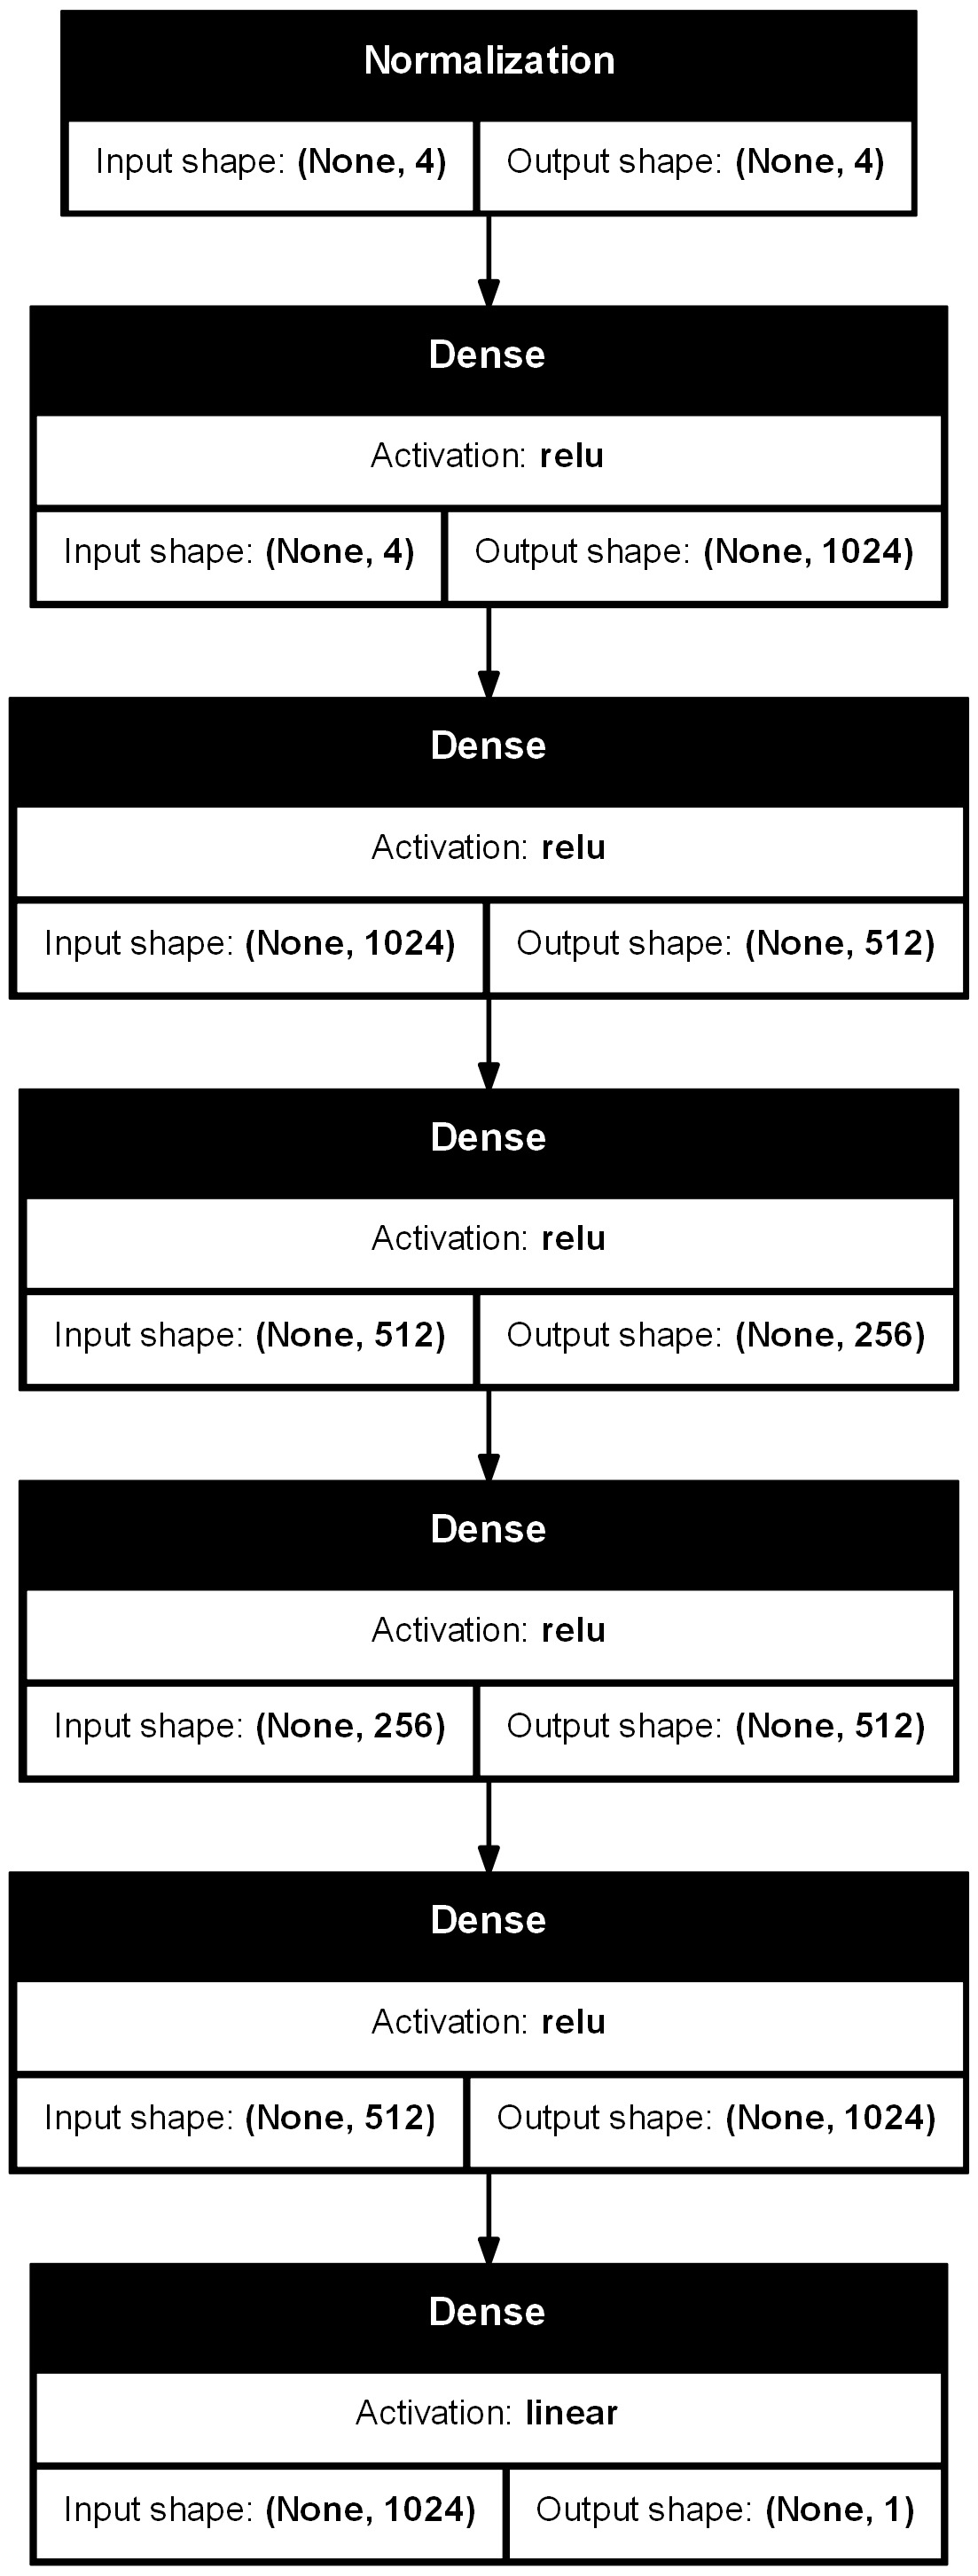
\includegraphics[width=0.38\textwidth]{tunedmodel_24_09_2024/structure.png} 
  \caption{Δομή βελτιστοποιημένου Νευρωνικού Δικτύου.}
  \label{fig:HypertunedStructure}
\end{figure}


\begin{figure}[H]
  \centering
  \subfloat[\textlatin{training history}]{\includesvg[width=0.5\textwidth]{tunedmodel_24_09_2024/traininghistory.svg}} \\
  \subfloat[$Y_{true}$ \textlatin{vs} $Y_{pred}$]{\includesvg[width=0.5\textwidth]{tunedmodel_24_09_2024/Ytrue_vs_Ypred.svg}}
  \subfloat[\textlatin{Residuals}]{\includesvg[width=0.5\textwidth]{tunedmodel_24_09_2024/Residuals_vs_Ytrue.svg}}

\caption{Απόδοση \textlatin{Hyperparameter tuned} Νευρωνικού δικτύου}
  \label{fig:HypertunedNNperf}
\end{figure}

Όπως φαίνεται από το \autoref{fig:HypertunedNNperf}, αυτό το μοντέλο εκπαιδεύτηκε για 200 \textlatin{epochs}, καθώς το MAE επικύρωσης σταματά να μειώνεται μετά από αυτό το σημείο. Αυτό το μοντέλο παρουσιάζει το χαμηλότερο MAE από όλα τα υπόλοιπα μοντέλα, με \(MAE < 5 m/s\) στην επικύρωση.

Επιπλέον, η κατανομή των δεδομένων γύρω από τη Γραμμή Μηδενικής Διαφοράς στο \autoref{fig:HypertunedNNperf} (γ'), είναι η πιο στενή από όλα τα μοντέλα, παράγοντας έτσι τα καλύτερα αποτελέσματα μέχρι στιγμής. Αξιοσημείωτο είναι επίσης ότι αυτό το μοντέλο έχει τον υψηλότερο αριθμό παραμέτρων που μπορούν να εκπαιδευτούν και απαιτεί τον περισσότερο χρόνο εκπαίδευσης.


    \chapter{Συμπεράσματα \& Μελλοντική Εργασία}
\label{conclusions-future-work}
\chapterprecis{Σε αυτό το κεφάλαιο παρουσιάζεται μια περίληψη των αποτελεσμάτων, εξάγονται γενικά συμπεράσματα και προτείνονται ιδέες για περαιτέρω ανάπτυξη.}

\section{Βελτιστοποίηση}\label{optimization}

Στο παρόν κεφάλαιο, παρουσιάζεται μια περίληψη των αποτελεσμάτων που παράχθηκαν σε αυτή την εργασία και εξάγονται γενικά συμπεράσματα επ' αυτών.

Στον \autoref{tab:flutter_results} παρατίθεται μια περίληψη των αποτελεσμάτων που αποκτήθηκαν με την εκάστοτε μέθοδο βελτιστοποίησης που χρησιμοποιήθηκε στην παρούσα εργασία, καθώς και ένας πίνακας, \autoref{tab:flutter_changes}, με την ποσοστιαία διαφορά από την αρχική ανάλυση.

\selectlanguage{english}
\begin{table}[h]
  \footnotesize
  \centering
  \setlength{\tabcolsep}{5pt}
  \renewcommand{\arraystretch}{1.2}
  \begin{tabularx}{\textwidth}{lccc}
      \toprule
      \textbf{Method} & \textbf{Flutter Velocity (m/s)} & \textbf{Mass (Kg)} & \textbf{Divergent Mode} \\
      \midrule
      Initial Flutter Characteristics & 94.11 & 67.33 & 3 \\
      Powell’s Method Scenario 1 & 99.48 & 67.33 & 3 \\
      Powell’s Method Scenario 2 & 175.28 & 67.33 & 3 \\
      Genetic Algorithm & 214.69 & 45.1 & 1 \\
      \bottomrule
  \end{tabularx}
  \caption{\textgreek{Σύνοψη των αποτελεσμάτων βελτιστοποίησης}}
  \label{tab:flutter_results}
\end{table}

\begin{table}[h]
  \centering
  \footnotesize
  \setlength{\tabcolsep}{5pt}
  \renewcommand{\arraystretch}{1.2}
  \begin{tabular}{lcc}
      \toprule
      \textbf{Method} & \textbf{Velocity Change (\%)} & \textbf{Mass Change (\%)} \\
      \midrule
      Powell’s Method Scenario 1 & 5.71\% & 0.00\% \\
      Powell’s Method Scenario 2 & 86.25\% & 0.00\% \\
      Genetic Algorithm & 128.13\% & -33.02\% \\
      \bottomrule
  \end{tabular}
  \caption{\textgreek{Σύγκριση των αποτελεσμάτων των μεθόδων βελτιστοποίησης}}
  \label{tab:flutter_changes}
\end{table}
\selectlanguage{greek}

Αυτό που είναι σαφές από τη σύνοψη των αποτελεσμάτων είναι ότι υπάρχει σημαντικός χώρος για βελτίωση σε σχέση με την αρχική λύση. 
Η επίδραση των γωνιών των στρώσεων είναι αξιοσημείωτη και κάτι που πρέπει να λαμβάνεται υπ' όψιν κατά το σχεδιασμό ενός φτερού αεροπλάνου με \textlatin{composite laminate} υλικά.
Αυτού του είδους η βελτιστοποίηση αξίζει να πραγματοποιείται, διότι μπορεί ενδεχομένως να μειώσει τη μάζα του αεροσκάφους, με αποτέλεσμα βελτιωμένες επιδόσεις πτήσης, χειρισμό και οικονομία καυσίμου.
Αξιοσημείωτο είναι, ωστόσο, ότι η δυναμική αστάθεια πτερυγισμού δεν είναι ο μόνος περιοριστικός παράγοντας για τη δομή της κύριας πτέρυγας και υπάρχουν άλλοι παράγοντες που πρέπει να ληφθούν υπ' όψιν. 
Ένας κύριος εξ αυτών είναι η παραμόρφωση της πτέρυγας και η δυναμική απόκριση υπό διαφορετικά φορτία και γωνίες προσβολής.
Ένας άλλος παράγοντας είναι τα φαινόμενα στατικής αεροελαστικότητας και η αντιστροφή του ελέγχου πτήσης.

Από τον \autoref{tab:flutter_changes} φαίνεται ότι το καλύτερο αποτέλεσμα επιτυγχάνεται με τη χρήση του γενετικού αλγορίθμου, ο οποίος καταφέρνει να μειώσει τη μάζα της πτέρυγας κατά
ένα διόλου αμελητέο $33\%$, ενώ ταυτόχρονα καταφέρνει να αυξήσει την ταχύτητα πτερυγισμού κατά $128\%$.
Αυτό το εντυπωσιακό αποτέλεσμα πρέπει να αντιμετωπιστεί με πολύ προσοχή, 
διότι όπως έχει συζητηθεί στην \autoref{genetic-algorithm-optimization}, η λύση φαίνεται
να καθίσταται ασταθής νωρίτερα, αν και το πρόσημο της απόσβεσης της πρώτης ιδιομορφής δεν αλλάζει μέχρι τα $214 m/s$.

\section{Πρόβλεψη με Νευρωνικά Δίκτυα}
\label{neural-network-prediction.}

Από την ανάπτυξη Νευρωνικών Δικτύων για την πρόβλεψη της ταχύτητας πτερυγισμού αυτής της γεωμετρίας, 
καταλήξαμε στο συμπέρασμα ότι απαιτείται ένα αρκετά περίπλοκο νευρωνικό δίκτυο 
για μία ικανοποιητική ακρίβεια στις προβλέψεις.

Επιπρόσθετα, τα δεδομένα που απαιτούνται για την εκπαίδευση του νευρωνικού, 
είναι υπολογιστικά ασύμφορο να αποκτηθούν και, 
στις περισσότερες περιπτώσεις, η υπολογιστική πολυπλοκότητα για τη δημιουργία 
των δεδομένων εκπαίδευσης ξεπερνά κατά πολύ
την αντίστοιχη για την πραγματοποίηση μιας άμεσης βελτιστοποίησης.

Η ακρίβεια των προβλεπόμενων αποτελεσμάτων είναι αρκετά καλή στις περισσότερες περιπτώσεις, 
αλλά όχι αρκετή για ακριβή πρόβλεψη πτερυγισμού σε κάθε περίπτωση, 
διότι υπάρχουν μερικά \textlatin{outliers} στα δεδομένα όπου η πρόβλεψη δεν είναι ικανοποιητική.

Αξιοσημείωτο είναι ότι μετά την εκπαίδευση του μοντέλου, απαιτείται σχεδόν μηδενικό
υπολογιστικό κόστος για να πραγματοποιηθεί μια πρόβλεψη σχετικά με την ταχύτητα πτερυγισμού. 
Το Νευρωνικό Δίκτυο μπορεί στη συνέχεια να χρησιμοποιηθεί για τη βελτιστοποίηση της κατασκευής, αν και η ακρίβεια των αποτελεσμάτων δεν είναι εγγυημένη.


\section{Μελλοντική Εργασία}\label{future-work}

Η παρούσα μελέτη παρέχει κάποιες εφαρμοσμένες πρακτικές και ερμηνείες στην ανάλυση πτερυγισμού και τις τεχνικές 
προσαρμογής πτερυγισμού χρησιμοποιώντας μεθόδους βελτιστοποίησης και \textlatin{Python}, αλλά 
παραμένουν αρκετές ανεξερεύνητες περιοχές που θα μπορούσαν να διαλευκανθούν με περαιτέρω μελέτη.

Οι μελλοντικές προσπάθειες θα πρέπει να περιλαμβάνουν τουλάχιστον μια πειραματική 
επικύρωση των αποτελεσμάτων της προσομοίωσης. Με αυτόν τον τρόπο, η επίδραση των 
γωνιών των στρώσεων του σύνθετου υλικού μπορεί να επιβεβαιωθεί στην πράξη.

Αν και πολλοί αλγόριθμοι βελτιστοποίησης χρησιμοποιήθηκαν σε αυτή τη μελέτη με 
υποσχόμενα αποτελέσματα, παραμένουν ανεξερεύνητες πολλές προηγμένες τεχνικές. 
Κάποια μελλοντική εργασία θα μπορούσε να εξετάσει αυτούς τους πιο πολυδιάστατους 
αλγορίθμους, καθώς και την ενδεχόμενη εφαρμογή μεθόδων βασισμένων στη μηχανική μάθηση
για περαιτέρω ενίσχυση των διαδικασιών βελτιστοποίησης.

Το φαινόμενο του πτερυγισμού που μελετήθηκε σε αυτή τη διατριβή, μοντελοποιημένο με 
την αεροδυναμική θεωρία \textlatin{Vortex Lattice} σε συνδυασμό με έναν επιλυτή 
βασισμένο στην ανάλυση ιδιομορφών, θα μπορούσε επίσης να προσομοιωθεί μέσω μιας 
\textlatin{transient} ανάλυσης αλληλεπίδρασης Ρευστού-Κατασκευής \textlatin{(FSI)}. Αυτό θα επέτρεπε μια 
σύγκριση των αποτελεσμάτων μεταξύ των δύο προσεγγίσεων, παρέχοντας περαιτέρω 
επικύρωση και σύγκριση των αποτελεσμάτων διαφορετικών μεθόδων.

Τέλος, η ενσωμάτωση των Νευρωνικών Δικτύων Ενημερωμένων από Φυσική \textlatin{(PINNs)} 
σε αυτή την εφαρμογή, πρόκειται για μια υποσχόμενη κατεύθυνση για μελλοντική έρευνα. 
Τα \textlatin{PINNs} είναι ένας αναδυόμενος κλάδος της υπολογιστικής μηχανικής, που συνδυάζει την εκμάθηση 
βασισμένη σε δεδομένα με τους φυσικούς νόμους που διέπουν την εκάστοτε εφαρμογή, όπως οι εξισώσεις 
της ροής ρευστού και της δομικής δυναμικής. Ενσωματώνοντας τη φυσική άμεσα στη 
διαδικασία εκπαίδευσης του νευρωνικού δικτύου, τα \textlatin{PINNs} μπορούν να προσφέρουν 
μια πιο αποτελεσματική και ακριβή λύση σε περίπλοκα προβλήματα αλληλεπίδρασης 
ρευστού-κατασκευής. Η δυνατότητά τους να παρακάμψουν κάποιους από τους περιορισμούς 
των παραδοσιακών αριθμητικών μεθόδων, όπως η δημιουργία πλέγματος και τα 
ζητήματα σύγκλισης του επιλυτή, τα καθιστά ιδιαίτερα ελκυστικά για τη μελέτη μηχανικών συστημάτων.


    
    \pagestyle{plain}
    \bibliography{references.bib}
    \appendix
\chapter{Python Code for Optimization}
\label{appendix}

In this appendix the main code for the simplest case of optimization
using Powell's method is presented. The code for all the other
applications is modified but the core logic and many parts remain the
same throughout. All the code including the code used to process the
results and produce the graphics in this thesis is available on GitHub:
\href{https://github.com/vasxen/Aeroelastic_Flutter}{vasxen/Aeroelastic\_Flutter
(github.com)}.
% Define VS Code-style colors
\definecolor{vscode_bg}{rgb}{0.16, 0.16, 0.16}      % Dark gray background
\definecolor{vscode_keyword}{rgb}{0.86, 0.36, 0.07} % Orange keywords
\definecolor{vscode_string}{rgb}{0.67, 0.83, 0.27}  % Green strings
\definecolor{vscode_comment}{rgb}{0.5, 0.5, 0.5}    % Gray comments
\definecolor{vscode_funcname}{rgb}{0.25, 0.72, 0.85} % Blue function names
\definecolor{vscode_number}{rgb}{0.79, 0.43, 0.07}  % Orange numbers

% Define VS Code-style Python listing
\lstdefinestyle{vscodepython}{
    language=Python,
    backgroundcolor=\color{white}, 
    basicstyle=\ttfamily\footnotesize\color{black}, % White text
    keywordstyle=\color{vscode_keyword}\bfseries, 
    stringstyle=\color{vscode_string}, 
    commentstyle=\color{vscode_comment}\itshape, 
    numberstyle=\color{vscode_number},
    identifierstyle=\color{black}, % Default text color for variables
    emph={self}, emphstyle=\color{vscode_funcname}, % Highlight "self" in blue
    frame=single, 
    rulecolor=\color{vscode_bg}, 
    numbers=left, 
    numbersep=5pt, 
    stepnumber=1, 
    breaklines=true, 
    showstringspaces=false, 
    tabsize=4
}
\lstinputlisting[style=vscodepython, caption={Python script for data processing}, label={lst:python_script}]{C:/Users/vasxen/OneDrive/Thesis/code/optimization.py}

\end{document}